% ------------------------------------------------------------------------
%
% -------------------      Plantilla_UIS.tex       -----------------------
%
% ------------------------------------------------------------------------
% ------------------------------------------------------------------------
% ------------------------------------------------------------------------
% Versión de plantilla para realización de informes de trabajo de grado
% construida para uso de la Universidad Industrial de Santander.
%
% Reservados todos los derechos
%
% Bucaramanga, Colombia
%
% Septiembre 17 de 2018
%
% ------------------------------------------------------------------------
% ------------------------------------------------------------------------
% ------------------------------------------------------------------------
%
% ------------------------------------------------------------------------
\documentclass[letterpaper,oneside,12pt,spanish]{report}          % Encabezados
\usepackage[utf8]{inputenc}
\usepackage{csquotes}
\usepackage[spanish]{babel}

% ------------------------------------------------------------------------
\usepackage{icontec_style}                   % Libreria UIS ICONTEC
% ------------------------------------------------------------------------
% Ingrese en este punto las librerías específicas de usuario
% ------------------------------------------------------------------------
\usepackage{amsmath, amsthm, amssymb}
\usepackage{subfigure}
\usepackage{float}
\usepackage{graphicx}
\usepackage{tabularx}
\usepackage{array}
\usepackage{booktabs}

\usepackage{tikz}
\usetikzlibrary{calc, spy, positioning, fit}

\usepackage{multirow}

\setcounter{tocdepth}{4} % show also subsections in toc
\setcounter{secnumdepth}{4} % show also subsections number in toc

% ------------------------------------------------------------------------
% Archivo de bibliografía
% ------------------------------------------------------------------------

\addbibresource{references.bib}
% ------------------------------------------------------------------------
\def\autora{CAMILO ERNESTO SERRANO LOZADA}
\def\autorb{OSCAR MAURICIO CAMPOS SEPULVEDA}
\def\titulo{Detección de retinopatía diabética en imágenes del fondo del ojo utilizando algoritmos de aprendizaje profundo}
\def\director{Jorge Villamizar Morales}
\def\directortitulo{Doctor en Ciencias Aplicadas}
\def\codirectora{Lola Xiomara Bautista Rozo}
\def\codirectoratitulo{Ph.D. en Automatización, tratamiento de señales e imágenes}
\def\universidad{Universidad Industrial de Santander}
\def\escuela{Escuela de Ingeniería de Sistemas e Informática}
\def\facultad{Facultad de Ingenierías Fisicomecánicas}
%\def\grupo{Grupo de Investigación en Diseño de Algoritmos y Procesamiento de Datos Multidimensionales (HDSP)}
\def\fecha{2025}
% \def\codigo{2171767} 

\newcolumntype{Y}{>{\centering\arraybackslash}X} % definir columna centrada

\begin{document}

% Inicio de documento
% ------------------------------------------------------------------------
% Definición silábica de palabras
% ------------------------------------------------------------------------
\hyphenation{pro-por-cio-nal di-se-ño}
\hypersetup {pdfborder = {0 0 0}}

% ------------------------------------------------------------------------
% Elementos previos al contenido del trabajo
% ------------------------------------------------------------------------
% ------------------------------------------------------------------------
%                                 Portada
% ------------------------------------------------------------------------

\thispagestyle{empty}

\begin{center}

\MakeUppercase{\titulo} \vspace{7.2cm}

\MakeUppercase{\autora}\\
\MakeUppercase{\autorb}\\
\vspace{7.2cm}

\MakeUppercase{\universidad}\\
\MakeUppercase{\facultad}\\
\MakeUppercase{\escuela}\\
BUCARAMANGA\\
2026\\

\end{center}

% ------------------------------------------------------------------------
%                              Contraportada
% ------------------------------------------------------------------------

\newpage
\thispagestyle{empty}

\begin{center}

\MakeUppercase{\titulo} \vspace{1.2cm}

\MakeUppercase{\autora}\\
\MakeUppercase{\autorb}\\

\vspace{2.0cm}

Trabajo de Grado para optar al título de\\
Ingeniero de Sistemas\\\vspace{2.5cm}

Director:\\
\director\\
{\directortitulo}\vspace{0.5cm}

Codirector:\\
\codirectora\\
{\codirectoratitulo}\vspace{2.5cm}

\MakeUppercase{\universidad}\\
\MakeUppercase{\facultad}\\
\MakeUppercase{\escuela}\\
BUCARAMANGA\\
2026\\

\end{center}

% ------------------------------------------------------------------------
  %Portada,contraportada,formato de nota,autorización
% ------------------------------------------------------------------------
% ------------------------------------------------------------------------
% ------------------------------------------------------------------------
% ------------------------------------------------------------------------
%                               Dedicatoria
% ------------------------------------------------------------------------
% ------------------------------------------------------------------------
% ------------------------------------------------------------------------
\chapter*{DEDICATORIA}

%\textbf{Por cambiar [...]}

\begin{flushright}
\textit{
Este trabajo está dedicado a mi  \\
familia, por su amor, apoyo incondicional \\
y por ser mi fuente constante de inspiración. \\
A mis padres, que con su ejemplo me enseñaron\\ 
el valor del esfuerzo y la perseverancia.  \\
A mis amigos, por su compañía y por \\
estar siempre ahí en los \\
momentos difíciles.
}
\end{flushright}

% ------------------------------------------------------------------------                                     % Dedicatoria
% ------------------------------------------------------------------------
% ------------------------------------------------------------------------
% ------------------------------------------------------------------------
% ------------------------------------------------------------------------
%                             AGRADECIMIENTOS
% ------------------------------------------------------------------------
% ------------------------------------------------------------------------
% ------------------------------------------------------------------------
\chapter*{AGRADECIMIENTOS}

La realización de este trabajo de grado representa la culminación de un extenso proceso formativo e investigativo. Este logro no habría sido posible sin el invaluable respaldo, la orientación experta y el constante apoyo de un grupo de personas a quienes deseamos expresar nuestro más profundo agradecimiento.
En primer lugar, dirigimos nuestra profunda gratitud a nuestro Director el profesor Jorge Villamizar Morales, y a nuestra Codirectora, la profesora Lola Bautista. Su experta dirección, sus sabios consejos y su constante disponibilidad para resolver nuestras inquietudes fueron el faro que guió este trabajo desde su concepción hasta su finalización. De manera muy especial, queremos agradecer a nuestro tutor Sebastian Carrillo y el profesor Ivan Ortiz, cuyo acompañamiento meticuloso y apoyo práctico fueron fundamentales en el desarrollo diario de este proyecto. Su paciencia para despejar nuestras dudas y su motivación en los momentos más desafiantes fueron un pilar fundamental para mantener el rumbo y superar los obstáculos.
A nuestros profesores, por haber sembrado en nosotros las bases del conocimiento y la pasión por la ingeniería a lo largo de toda nuestra carrera.
A nuestras familias, por ser nuestro soporte inquebrantable. A nuestros padres, por su amor incondicional, por sus sacrificios y por creer siempre en nosotros. Este logro es tan nuestro como suyo.
A nuestros amigos y compañeros de universidad, por los momentos de colaboración, por las palabras de aliento y por hacer de este camino una experiencia memorable.
Finalmente, a todos aquellos que, de una u otra forma, contribuyeron a la realización de este sueño, les extendemos nuestro más sentido agradecimiento.
% ------------------------------------------------------------------------
\newpage                            % Agradecimientos
% ------------------------------------------------------------------------
\tableofcontents                                          % Tabla de contenido
% ------------------------------------------------------------------------
\listoffigures                             % Lista de figuras, tablas y anexos
\listoftables                                                    %\listofanexo
% ------------------------------------------------------------------------
%\input{Secs/Glosario}                                  % Glosario de términos
% ------------------------------------------------------------------------
% Contenido del Informe
% ------------------------------------------------------------------------
% ------------------------------------------------------------------------
% ------------------------------------------------------------------------
% ------------------------------------------------------------------------
%                                Resumen
% ------------------------------------------------------------------------
% ------------------------------------------------------------------------
% ------------------------------------------------------------------------
\chapter*{RESUMEN}

\footnotesize{
  \begin{description}
    \item[TÍTULO:] \MakeUppercase{\titulo}
          \astfootnote{Trabajo de grado}
    \item[AUTOR:]{\autora}, {\autorb}
          \asttfootnote{\facultad. \escuela. Director: \director. Codirectores:
          \codirectora}
    \item[PALABRAS CLAVE:] RETINOPATÍA DIABÉTICA, REDES NEURONALES CONVOLUCIONALES,
    APRENDIZAJE PROFUNDO, IMÁGENES DEL FONDO DEL OJO, PROCESAMIENTO DIGITAL DE IMÁGENES,
    APRENDIZAJE POR TRANSFERENCIA.
    \item[DESCRIPCIÓN:] \hfill \\
          La retinopatía diabética (RD) es una complicación microvascular causada por
          daños en los vasos sanguíneos de la retina debido a niveles elevados de azúcar en sangre,
          común en personas con diabetes y es considerada una de las principales causas de
          ceguera en el mundo. Esta enfermedad suele diagnosticarse mediante exámenes oculares en
          los que se evalúa el fondo del ojo. Sin embargo, el diagnóstico manual es desafiante
          porque es costoso y consume tiempo, lo que limita su acceso en áreas con pocos
          recursos médicos. Esto hace necesario buscar métodos automatizados que permitan
          una detección más rápida y precisa de la enfermedad. Este trabajo desarrolla modelos 
          basados en redes neuronales convolucionales (CNN) para detectar la enfermedad y clasificar
          sus niveles de severidad mediante clasificadores binarios (presencia/ausencia) y multiclase
          (cinco niveles). Se utilizó aprendizaje por transferencia con las arquitecturas MobileNetV2, 
          ResNet50V2, InceptionV3 y VGG19, entrenadas con 35.121 imágenes del dataset público de Kaggle. 
          El preprocesamiento incluyó normalización de color, enmascaramiento periférico, balanceo de 
          clases mediante submuestreo y aumento de datos, incorporando bloques Multi-Head Attention, 
          capas GaussianNoise y técnicas de regularización (Dropout, L2, early stopping). El modelo 
          fue evaluado mediante sensibilidad, precisión, F1-score y AUC-ROC, siendo MobileNetV2 el 
          modelo de mejor desempeño, alcanzando una sensibilidad de 96,5\% en clasificación binaria 
          con intervalos de confianza (IC95\%: AUC-ROC 0.9636 - 0.99). Para clasificación multiclase,
          se alcanzó una sensibilidad de 65\%, identificando el canal verde como el más efectivo debido
          a su contraste para lesiones hemorrágicas. La validación externa en datasets MESSIDOR-2, 
          IDRiD y FOSCAL confirmó la capacidad de generalización del modelo, demostrando su viabilidad 
          como herramienta de apoyo al tamizaje clínico de retinopatía diabética.      
  \end{description}}\normalsize
% ------------------------------------------------------------------------                                           % Resumen

\chapter*{ABSTRACT}

\footnotesize{
\begin{description}
  \item[TITLE:] \MakeUppercase{Detection of Diabetic Retinopathy in Fundus Images Using Deep Learning Algorithms.}
  \astfootnote{Bachelor Thesis}
  \item[AUTHOR:] {\autora}, {\autorb}
  \asttfootnote{\facultad. \escuela. Advisor: \director. Co-advisor: \codirectora}
  \item[KEYWORDS:] DIABETIC RETINOPATHY, CONVOLUTIONAL NEURONAL NETWORKS, DEEP LEARNING, FUNDUS IMAGES, DIGITAL IMAGE PROCESSING, TRANSFER LEARNING.
  \item[DESCRIPTION:]\hfill \\  Diabetic retinopathy (DR) is an ocular complication caused by damage to the blood vessels in the retina due to elevated blood sugar levels, commonly found in people with diabetes. It is considered one of the leading causes of blindness worldwide, highlighting the importance of early diagnosis to prevent or minimize visual impairment. This disease is typically diagnosed through eye exams that assess the retina. However, manual diagnosis is challenging because it is costly and time-consuming, limiting access in areas with scarce medical resources. This underscores the need for automated methods that enable faster and more accurate disease detection. This study proposes two models based on convolutional neural networks (CNNs) that not only detect the disease but also classify its different severity levels. The model is trained using a public dataset and later tested with a private dataset provided by the Santander Ophthalmological Foundation. This study addresses the issue of data imbalance through preprocessing and image augmentation techniques. Additionally, various architectures are built using pretrained networks to extract features from the images. The models performance is evaluated and compared using different metrics, where the best binary classification model achieves a sensitivity of 96.5\%, and the best multiclass classification model reaches 76.8\%

\end{description}}\normalsize
% ------------------------------------------------------------------------ 
                                        % Abstract


% ------------------------------------------------------------------------
% Capítulos
% ------------------------------------------------------------------------
% Introducción

\nnchapter{INTRODUCCIÓN} \label{chap:introduccion}

La diabetes mellitus (DM) es una enfermedad metabólica crónica que se caracteriza por
niveles elevados de glucosa en la sangre. Esto ocurre cuando el cuerpo no produce
suficiente insulina, una hormona producida por el páncreas que regula la cantidad de
glucosa en la sangre, o cuando las células no responden adecuadamente a la insulina.
Alrededor de 463 millones de adultos entre 20 y 79 años tienen diabetes mellitus (DM) en
la actualidad, lo que representa el 9.3\% de la población mundial en este grupo de edad
\myfootcite{antonetti2021current}.

La retinopatía diabética (RD) es una complicación
microvascular específica de la diabetes mellitus (DM) que afecta a 1 de cada 3 personas
con esta enfermedad, dañando los vasos sanguíneos de la retina y convirtiéndose en una de
las principales causas de pérdida de visión en la población adulta activa. Los pacientes
con niveles graves de RD experimentan una calidad de vida significativamente reducida y
niveles más bajos de bienestar físico, emocional y social. Frente a este panorama, el 
presente trabajo propone el desarrollo de un algoritmo de
clasificación basado en aprendizaje profundo, específicamente mediante redes neuronales
convolucionales (CNN), para la detección de retinopatía diabética en imágenes del fondo
del ojo. 

Este proyecto utiliza estas redes en la construcción de clasificadores binarios
(presencia o ausencia de la enfermedad) y multiclase (cinco niveles de severidad), dado que
este enfoque combinado ha mostrado obtener resultados prometedores tanto para tamizaje como
para gradación clínica. El modelo binario permite una rápida detección de la enfermedad,
optimizando el tiempo de diagnóstico y brindando una solución viable para su implementación en
escenarios de alta demanda, como en áreas con recursos limitados. Por su parte, los
clasificadores multiclase aportan valor adicional en términos de tratamiento personalizado y
seguimiento de los pacientes al distinguir entre los diferentes grados de severidad de la retinopatía
diabética.

Una de las principales contribuciones de este proyecto es la experimentación con diferentes
configuraciones de redes neuronales, explorando cómo las variaciones en el preprocesamiento
y las arquitecturas afectan el desempeño del modelo. Se implementaron y compararon cuatro
arquitecturas preentrenadas: MobileNetV2, ResNet50V2, InceptionV3 y VGG19, utilizando
aprendizaje por transferencia con 35.121 imágenes del dataset de Kaggle para entrenamiento
y datasets externos (MESSIDOR-2, IDRiD, FOSCAL) para validación. Un aspecto distintivo es
el análisis de imágenes a través de los tres canales de color RGB (rojo, verde y azul) de
forma independiente, un enfoque que no ha sido ampliamente explorado en investigaciones
previas. La idea es determinar cuál de estos canales, por separado, proporciona la mejor
representación de las características relevantes para la detección de la RD. Este análisis
permitió identificar el canal verde como el más efectivo para la clasificación multiclase
debido a su mejor contraste para lesiones hemorrágicas.

Adicionalmente, se implementaron distintas técnicas de regularización, como Dropout,
regularización L2, capas GaussianNoise, bloques Multi-Head Attention y Data Augmentation,
con el fin de reducir el sobreajuste y mejorar la generalización del modelo. Estas técnicas
se evaluaron de manera exhaustiva para identificar cuáles son más efectivas en el contexto
específico de clasificación de imágenes de retinopatía diabética. La combinación de estas
estrategias no solo mejoró el rendimiento del modelo, sino que también contribuyó a
desarrollar un sistema robusto y adaptable a diferentes tipos de datos, mejorando su
aplicabilidad en diversas poblaciones. Este trabajo logró una sensibilidad de 96.5\%
en clasificación binaria (con intervalos de confianza bootstrap del 95\%: AUC-ROC 0.9636–0.9936)
y 65\% de sensibilidad en clasificación multiclase, demostrando la viabilidad de estas
tecnologías para tamizaje automatizado.

Esta investigación busca impulsar el uso de tecnologías recientes en salud ocular. Su
aplicación permitirá abordar la falta de especialistas en oftalmología, promover la
detección oportuna de enfermedades y ampliar el alcance del diagnóstico, optimizando
así la eficiencia y accesibilidad de los servicios de salud visual. Además, esta
metodología podría sentar las bases para implementar soluciones similares en otros países
en vías de desarrollo, generando un impacto significativo en la calidad de vida de los
pacientes.

El presente documento se estructura de la siguiente manera: en el Capítulo 1 se plantea
el problema que motiva este trabajo; el Capítulo 2 detalla los objetivos; los Capítulos 3
y 4 presentan el marco teórico y los antecedentes; el Capítulo 5 describe la metodología
implementada; el Capítulo 6 expone los resultados obtenidos; finalmente, los Capítulos 7,
8 y 9 presentan la discusión, conclusiones y recomendaciones respectivamente.

 % Introducción
\input{secciones/planteamiento_problema.tex} % Planteamiento del problema
% ------------------------------------------------------------------------
% ------------------------------------------------------------------------
% ------------------------------------------------------------------------
%                              Objetivos
% ------------------------------------------------------------------------
% ------------------------------------------------------------------------
% ------------------------------------------------------------------------

\chapter{OBJETIVOS} \label{chap:objetivos}

\subsection*{Objetivo general}

\begin{itemize}

    \item Desarrollar un algoritmo de clasificación basado en aprendizaje profundo para la
    detección de retinopatía diabética en imágenes del fondo del ojo.
    
\end{itemize}

\subsection*{Objetivos específicos}


\begin{enumerate}

    \item Realizar una revisión de la literatura científica sobre la detección de la
    retinopatía diabética utilizando técnicas de aprendizaje profundo en imágenes del
    fondo del ojo.

    \item Recopilar y organizar un conjunto de datos clínicos de imágenes del fondo del
    ojo para el entrenamiento y evaluación del modelo.

    \item Desarrollar un algoritmo para la clasificación de retinopatía diabética
    utilizando redes neuronales convolucionales.

    \item Evaluar y validar la efectividad del sistema de detección, comparándolo con
    otros sistemas análogos y a la vanguardia de la detección de retinopatía diabética a
    través de aprendizaje profundo.

\end{enumerate}

\subsection*{Trazabilidad de objetivos}

La Tabla~\ref{tab:trazabilidad-objetivos} indica en qué secciones del documento se
evidencia el cumplimiento de cada objetivo específico.

\begin{table}[H]
\centering
\renewcommand{\arraystretch}{1.3}
\caption{Trazabilidad de los objetivos específicos}
\label{tab:trazabilidad-objetivos}
\begin{tabularx}{\textwidth}{c X l}
\hline
\textbf{OE} & \textbf{Objetivo específico} & \textbf{Sección(es)} \\ \hline
1 & Realizar una revisión de la literatura científica sobre la detección de la
retinopatía diabética utilizando técnicas de aprendizaje profundo en imágenes del fondo
del ojo. &
Cap.~\ref{chap:fundamentos}, Cap.~\ref{chap:trabajos-previos} \\
2 & Recopilar y organizar un conjunto de datos clínicos de imágenes del fondo del ojo
para el entrenamiento y evaluación del modelo. &
Sec.~\ref{sec:conjuntos-datos}, Sec.~\ref{sec:preprocesamiento} \\
3 & Desarrollar un algoritmo para la clasificación de retinopatía diabética utilizando
redes neuronales convolucionales. &
Sec.~\ref{sec:arquitecturas-cnn}, Sec.~\ref{sec:config-experimental} \\
4 & Evaluar y validar la efectividad del sistema de detección, comparándolo con otros
sistemas análogos y a la vanguardia de la detección de retinopatía diabética a través de
aprendizaje profundo. &
Cap.~\ref{chap:resultados}, Sec.~\ref{subsec:comparacion-literatura},
Cap.~\ref{chap:discusion} \\ \hline
\end{tabularx}
\caption*{\textit{Fuente: Elaboración propia}}
\end{table}

\pagebreak


% ------------------------------------------------------------------------
% ------------------------------------------------------------------------  % Objetivos
\chapter{FUNDAMENTOS} \label{chap:fundamentos}

El desarrollo de sistemas automatizados para la detección y clasificación de retinopatía
diabética mediante técnicas de aprendizaje profundo requiere una comprensión sólida de
múltiples dominios del conocimiento. Este capítulo presenta los fundamentos teóricos que
sustentan el presente trabajo, organizados en tres componentes principales: primero, se
describe la naturaleza y características de las imágenes de fondo de ojo, el principal
insumo del sistema propuesto; segundo, se expone la fisiopatología y clasificación
clínica de la retinopatía diabética; y tercero, se desarrollan los conceptos
fundamentales de inteligencia artificial, aprendizaje automático y redes neuronales
convolucionales que constituyen la base metodológica del trabajo.


\section{IMÁGENES DEL FONDO DE OJO}

Las imágenes de fondo de ojo, también conocidas como retinografías o imágenes de retina,
son fotografías detalladas de la parte posterior del ojo que permiten observar
estructuras clave como la retina, el nervio óptico, los vasos sanguíneos y la mácula.
Estas imágenes son fundamentales en oftalmología para el diagnóstico y seguimiento de
diversas enfermedades oculares, como la retinopatía diabética, el glaucoma, la
degeneración macular y otros trastornos retinianos. A través del análisis de estas
imágenes, los médicos pueden detectar alteraciones en los vasos sanguíneos, signos de
inflamación o daño estructural en la retina, lo que puede ser indicativo de enfermedades
en progresión.

El proceso de captura de estas imágenes se realiza mediante un examen médico no invasivo,
en el cual se emplea un oftalmoscopio o una cámara de fondo de ojo especializada. Este
instrumento emite una luz que atraviesa las pupilas y permite al especialista examinar
directamente la retina, los vasos sanguíneos y el nervio óptico. En la mayoría de los
casos, se requiere la dilatación de las pupilas para mejorar la visualización,
especialmente si se utiliza una cámara de fondo de ojo avanzada. Aunque la captura de
estas imágenes no es dolorosa, puede llevar algunos minutos, dependiendo de la tecnología
utilizada.

Existen varias técnicas para realizar la oftalmoscopia, cada una con sus características
y ventajas. La importancia de estas imágenes en la práctica clínica es incuestionable. En
algunos estudios \myfootcite{wong2008prevalence} se ha destacado cómo el análisis de la
imagen del fondo de ojo es crucial para la detección temprana de la retinopatía
diabética, lo que permite la intervención oportuna y la prevención de la pérdida de
visión. Esta capacidad de detectar cambios sutiles en la estructura ocular antes de que
se presenten síntomas graves resalta la utilidad de las imágenes de fondo de ojo en la
medicina preventiva.

\begin{figure}[H]
    \centering
    \caption{Imagen del fondo de ojo mostrando estructuras anatómicas principales}
    \label{fig:fundus-image}
    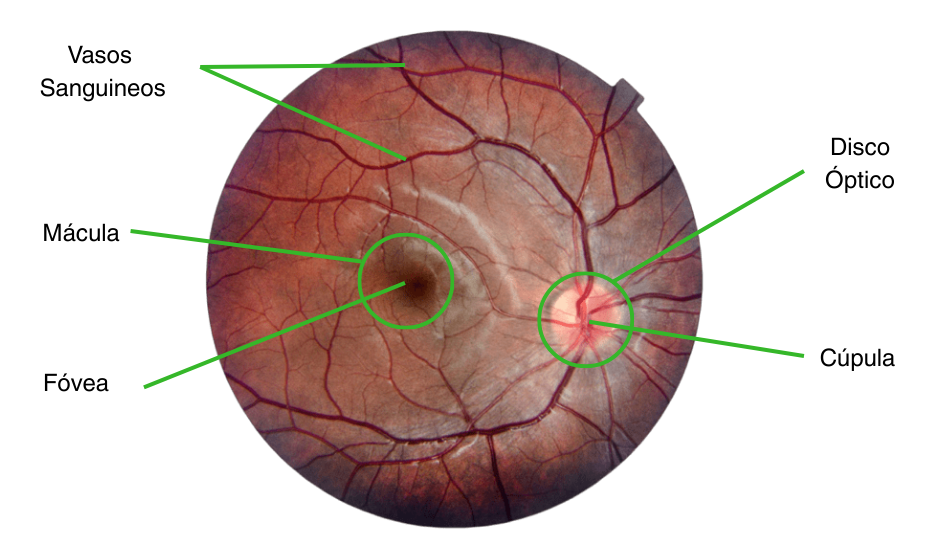
\includegraphics[width=1\textwidth]{imágenes/marco teórico/fundus image.png}
    \caption*{\textit{Fuente: Elaboración propia}}
\end{figure}

En la actualidad podemos encontrar otros tipos de exámenes que pueden ayudar a detectar
la retinopatía diabética. Entre los más conocidos está el examen con lámpara de
hendidura, que permite observar la parte frontal del ojo y la retina; y la tomografía de
coherencia óptica (OCT), que toma secciones transversales de la retina y es útil para
evaluar el grosor y detectar edema macular. Sin embargo, las imágenes del fondo de ojo
son las más utilizadas en la detección de la RD debido a que proporcionan una
visualización directa de la retina, donde se producen los cambios patológicos
característicos, y son relativamente fáciles de interpretar, lo que permite un
diagnóstico rápido. Además, con el avance de la inteligencia artificial, estas imágenes
pueden ser analizadas automáticamente mediante algoritmos de aprendizaje profundo,
permitiendo un tamizaje masivo y eficiente.

\section{RETINOPATÍA DIABÉTICA}

La retinopatía diabética es una complicación ocular de la diabetes que se produce debido
al daño en los vasos sanguíneos de la retina, el tejido sensible a la luz en la parte
posterior del ojo. Este daño es causado principalmente por niveles elevados de glucosa en
la sangre, que pueden obstruir los pequeños vasos sanguíneos que alimentan la retina.
Este daño hace que los vasos sanguíneos se vuelvan más permeables y propensos a filtrar
líquido y sangre en la retina. Además, los vasos sanguíneos pueden hincharse y formar
microaneurismas, que son pequeñas protuberancias en los vasos sanguíneos que pueden
romperse y sangrar.

Esta enfermedad puede tener consecuencias graves para la visión. Una de las
complicaciones más comunes es el sangrado dentro del ojo, que ocurre cuando se forman
vasos sanguíneos anormales que se rompen y liberan sangre en el interior del ojo. Este
sangrado puede hacer que la visión se vuelva borrosa o incluso se pierda completamente si
es muy grande. Otra complicación seria es el desprendimiento de la retina. Los vasos
sanguíneos anormales pueden generar tejido cicatricial que tira de la retina, lo que
puede hacer que se separe de la parte posterior del ojo.

\section{CLASIFICACIÓN DE LA RETINOPATÍA DIABÉTICA EN IMÁGENES DEL FONDO DE OJO}

Los signos microvasculares retinianos clásicos incluyen microaneurismas, hemorragias,
exudados duros, manchas de algodón, dilatación venosa y perlas, así como diversas
anomalías microvasculares intrarretinianas. En las etapas iniciales de la enfermedad,
muchos de estos síntomas no se manifiestan de manera evidente, lo que hace que el
diagnóstico temprano sea más desafiante. Por esta razón, se recomienda que los pacientes
diabéticos se sometan a exámenes regulares de fondo de ojo, incluso si no experimentan
síntomas. La detección temprana es fundamental, ya que permite la intervención antes de
que la enfermedad progrese, lo que brinda una mayor oportunidad para un tratamiento
eficaz, reduce el riesgo de ceguera y atenúa las complicaciones asociadas a la
retinopatía diabética.

La retinopatía diabética se clasifica en dos formas principales: la retinopatía diabética
no proliferativa (RDNP) y la retinopatía diabética proliferativa (RDP), cada una con
características particulares que influyen en el manejo clínico y el pronóstico de la
enfermedad. En la RDNP, los cambios en los vasos sanguíneos retinianos son generalmente
más leves e incluyen microaneurismas, hemorragias y exudados duros. Aunque estos signos
pueden no afectar gravemente la visión en sus primeras etapas, la progresión sin
tratamiento adecuado puede derivar en la forma proliferativa.

El diagnóstico oportuno es crucial, ya que un control adecuado de los niveles de glucosa
en sangre y la detección temprana de la enfermedad pueden retrasar o incluso evitar el
avance hacia formas más graves de retinopatía. Además, estudios han demostrado que los
pacientes que se someten a exámenes regulares de fondo de ojo tienen una mejor tasa de
preservación de la visión a largo plazo \myfootcite{cusick2005associations}.

\begin{figure}[H]
    \centering
    \caption{Etapas de la retinopatía diabética: (a) leve, (b) moderada, (c) severa, (d)
proliferativa}
    \label{fig:etapas-rd}
    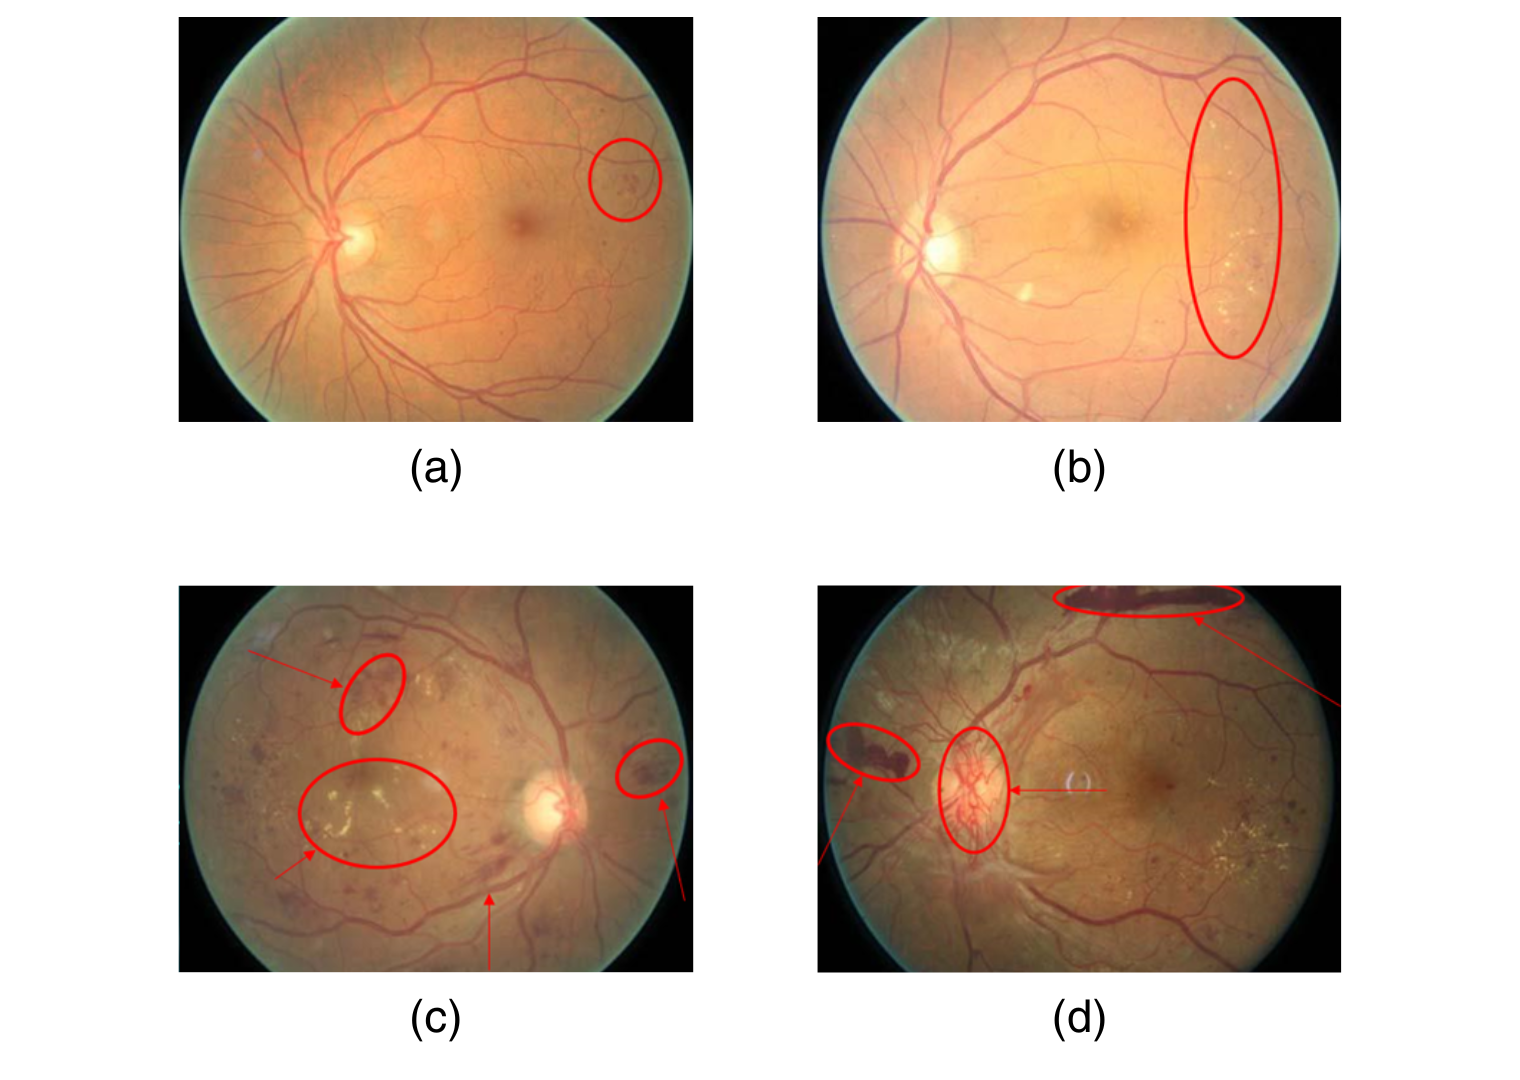
\includegraphics[width=1\textwidth]{imágenes/marco teórico/etapas RD.png}
    \caption*{\textit{Fuente: Adaptado de clasificación clínica estándar de retinopatía
diabética}}
\end{figure}

La retinopatía diabética no proliferativa progresa en varias etapas, como se observa en
la Figura~\ref{fig:etapas-rd}. En la etapa leve (Figura~\ref{fig:etapas-rd}a), los
pequeños vasos sanguíneos de la retina comienzan a debilitarse y desarrollan
microaneurismas, pequeñas protuberancias en las paredes de los vasos, y puede haber una
leve obstrucción que dificulta el suministro de oxígeno y nutrientes a la retina. En la
etapa moderada (Figura~\ref{fig:etapas-rd}b), el deterioro de los vasos sanguíneos se
intensifica, apareciendo más microaneurismas junto con pequeñas hemorragias y exudados,
que son acumulaciones de líquido y proteínas en la retina; también pueden observarse un
engrosamiento de las paredes de los vasos y una disminución en la circulación sanguínea.
En la etapa severa (Figura~\ref{fig:etapas-rd}c), los daños en los vasos sanguíneos son
más significativos, causando una disminución del flujo sanguíneo a la retina, hemorragias
mayores y exudados extensos, así como la formación de tejido fibroso que puede llevar a
la tracción y desprendimiento de la retina. Finalmente, en la etapa proliferativa o
retinopatía diabética proliferativa (RDP) (Figura~\ref{fig:etapas-rd}d), los nuevos vasos
sanguíneos crecen anormalmente en la retina, lo que crea presión en el globo ocular y
puede hacer que la retina se desprenda. Además, la sangre se filtra en el vítreo, lo que
daña el nervio óptico, responsable de transmitir imágenes al cerebro, provocando pérdida
de visión.

\begin{table}[H]
\centering
\renewcommand{\arraystretch}{1.5}
\caption{Etapas de la retinopatía diabética y sus manifestaciones clínicas observables en
oftalmoscopia}
\label{tab:etapas-rd}
\begin{tabularx}{\textwidth}{X X}
\hline
\textbf{Etapa} & \textbf{Hallazgos observables en la oftalmoscopia} \\ \hline
Sin retinopatía aparente & Sin anomalías \\
RD no proliferativa leve & Solo microaneurismas \\
RD no proliferativa moderada & Más microaneurismas \\
RD no proliferativa severa & Hemorragias intrarretinianas mayor a 20 en cada
cuadrante.\newline
Anomalías microvasculares intrarretinianas (en 1 cuadrante) \\
RD proliferativa & Neovascularización\newline
Hemorragia vítrea prerretiniana \\ \hline
\end{tabularx}
\end{table}

\section{INTELIGENCIA ARTIFICIAL}

El estudio de la inteligencia artificial (IA) ha sido una disciplina en constante
evolución durante más de 65 años, impulsada por el esfuerzo conjunto de científicos e
ingenieros. El principio fundamental detrás de la IA es que las máquinas, creadas por el
ser humano, pueden ir más allá de realizar tareas repetitivas o intensivas, desarrollando
una forma de inteligencia que imita o incluso supera ciertas capacidades humanas
\myfootcite{jiang2022quo}.

Uno de los aspectos más destacados de la IA es su capacidad para cambiar el paradigma
tradicional de los algoritmos. En la programación convencional, los datos de entrada son
procesados por un conjunto de reglas predefinidas por el programador, lo que da como
resultado una salida determinada. En contraste, los sistemas de inteligencia artificial
operan mediante un enfoque de aprendizaje automático, donde se proporcionan conjuntos de
datos de entrada y salida, pero el algoritmo debe aprender por sí mismo las reglas y
patrones subyacentes que relacionan ambos conjuntos. Esto permite que el programa sea
capaz de inferir correlaciones entre datos y, con el tiempo, adaptar su comportamiento,
mejorando su precisión y eficiencia sin intervención humana directa.

En el ámbito de la medicina, la inteligencia artificial ha mostrado un crecimiento
impresionante y continúa ganando terreno. Año tras año se incrementa su uso, a medida que
los avances en la ciencia computacional permiten desarrollar tecnologías más sofisticadas
y eficaces. Un ejemplo de ello son los robots quirúrgicos, que realizan procedimientos
con una precisión milimétrica, minimizando riesgos y mejorando los tiempos de
recuperación. Asimismo, se han creado sistemas de IA que analizan grandes cantidades de
datos clínicos para clasificar y diagnosticar enfermedades con una exactitud comparable a
la de los expertos humanos \myfootcite{gulshan2016development}. Además, la IA también se
está utilizando para predecir brotes epidémicos, personalizar tratamientos médicos y
mejorar la gestión de los servicios de salud en general. A medida que la investigación
avanza, es probable que veamos aplicaciones aún más innovadoras de la IA, que no solo
transformarán la manera en que abordamos la medicina, sino que también influirán en una
gran cantidad de otras industrias.

\subsection{APRENDIZAJE AUTOMÁTICO}

El aprendizaje automático (machine learning) es un subcampo de la inteligencia artificial
que ha transformado profundamente la manera en la que interactuamos con la tecnología. Se
refiere a la capacidad de las máquinas de aprender a partir de los datos que se les
proporcionan, sin necesidad de ser programadas de manera explícita para cada tarea
específica. Estos sistemas utilizan algoritmos matemáticos complejos para identificar
patrones dentro de grandes volúmenes de datos, y luego emplean esos patrones para hacer
predicciones o tomar decisiones autónomas.

El proceso de aprendizaje automático comienza con la recopilación de datos, que es
crucial para obtener resultados precisos. La calidad de los datos tiene una influencia
directa sobre el rendimiento del modelo, por lo que es fundamental que los datos sean
representativos, completos y correctos. En muchas ocasiones, los datos deben ser
preprocesados para asegurar que se encuentren en una forma adecuada para ser procesados
por los algoritmos, lo que incluye tareas como la normalización, la eliminación de
valores atípicos o la imputación de datos faltantes.

Existen diversos tipos de algoritmos de aprendizaje automático, entre los cuales destacan
la clasificación, regresión y clustering, y la selección del algoritmo adecuado depende
del tipo de problema que se desee resolver. Una vez que se cuenta con los datos
preparados, se procede a entrenar el modelo ajustando sus parámetros internos de manera
que se minimicen los errores en las predicciones. Durante este proceso, el modelo aprende
a realizar la tarea que se le ha asignado, mejorando su capacidad para generalizar a
datos que no haya visto previamente. Finalmente, el rendimiento del modelo se evalúa
utilizando un conjunto de datos de prueba, lo que permite verificar que el modelo sea
capaz de generalizar bien y no esté simplemente memorizando los datos de entrenamiento.

Dentro del campo del aprendizaje automático, existen diferentes tipos o enfoques según la
estructura de los datos y el tipo de tarea que se desea realizar. Los principales son: el
aprendizaje supervisado, el no supervisado, el semisupervisado y el aprendizaje por
refuerzo. En el aprendizaje supervisado se realiza el entrenamiento utilizando un
conjunto de datos etiquetado, es decir, datos para los cuales ya se conoce la salida
correcta. El objetivo es que el modelo pueda mapear nuevas entradas a sus respectivas
salidas correctas (etiquetas). Los modelos de clasificación y regresión son ejemplos
típicos de aprendizaje supervisado. En clasificación, el objetivo es asignar una etiqueta
a un conjunto de datos (por ejemplo, determinar si una imagen contiene un perro o un
gato), mientras que en regresión el objetivo es predecir un valor continuo (como el
precio de una casa en función de características como su tamaño y ubicación)
\myfootcite{jordan2015machine}.

Por otro lado, en el aprendizaje no supervisado el modelo trabaja con un conjunto de
datos que no tiene etiquetas, y el objetivo es identificar patrones ocultos dentro de los
datos. Por ejemplo, el modelo puede buscar agrupaciones de datos similares (clustering) o
intentar reducir la cantidad de características necesarias para representar los datos
(reducción de dimensionalidad). Este tipo de aprendizaje se utiliza ampliamente en
análisis exploratorio de datos y en tareas como la segmentación de clientes o la
detección de anomalías.

En el enfoque del aprendizaje semisupervisado se combinan elementos del aprendizaje
supervisado y no supervisado. En este caso, el conjunto de datos contiene tanto ejemplos
etiquetados como no etiquetados. Este enfoque es útil cuando etiquetar grandes cantidades
de datos es costoso o impráctico, pero se dispone de un pequeño conjunto de datos
etiquetados para guiar el proceso de aprendizaje. Los algoritmos semisupervisados
intentan aprovechar los datos no etiquetados para mejorar el rendimiento general del
modelo.

Por último, el aprendizaje por refuerzo se basa en el concepto de recompensa y
penalización. En este paradigma, un agente toma decisiones en un entorno y recibe
recompensas o penalizaciones en función de las acciones que realiza. El objetivo es que
el agente aprenda a tomar decisiones que maximicen la recompensa acumulada a largo plazo.
Este enfoque se utiliza en tareas complejas donde las decisiones deben tomarse en
secuencia, como en la robótica, el juego de ajedrez o la conducción autónoma.

\subsection{REDES NEURONALES CONVOLUCIONALES}

En el campo de la visión por computadora, las redes neuronales convolucionales (CNN, por
sus siglas en inglés) y sus posteriores mejoras han representado un hito crucial en el
procesamiento de imágenes. El uso de estas fue popularizado por el trabajo de Yann LeCun
y colaboradores en 1998 \myfootcite{lecun1998gradient}. Antes de la aparición de las CNN,
las redes neuronales artificiales tradicionales tenían limitaciones significativas para
trabajar con datos de más de una dimensión, como es el caso de las imágenes. Las redes
neuronales convencionales están diseñadas para procesar arreglos numéricos
unidimensionales. Estos arreglos no son ideales para procesar imágenes, las cuales, al
ser tratadas por un computador, se representan como matrices bidimensionales de valores
numéricos (en el caso de las imágenes en escala de grises) o tridimensionales (para
imágenes en color).

Para que una red neuronal tradicional pueda procesar imágenes, debe aplanar estas
matrices multidimensionales, convirtiéndolas en un arreglo unidimensional. Este proceso
implica perder la relación espacial entre los píxeles vecinos, lo que resulta en una
pérdida significativa de información contextual, esencial para tareas de clasificación y
detección de patrones. Como resultado, el modelo es menos efectivo al capturar
características importantes que dependen de la estructura espacial de los datos.

Mientras que las redes neuronales convolucionales resuelven este problema al procesar las
imágenes en su formato original de múltiples dimensiones. Una CNN utiliza una operación
denominada convolución, que consiste en aplicar un filtro (o kernel) a lo largo de la
imagen. Este filtro también es un arreglo de varias dimensiones que se desplaza sobre la
imagen, realizando una operación de multiplicación elemento a elemento entre el filtro y
las porciones de la imagen con las que coincide. El filtro "captura" patrones locales,
como bordes, texturas o formas, y extrae información relevante de estas coincidencias. Al
repetir este proceso a través de diferentes áreas de la imagen, se generan mapas de
características que preservan las relaciones espaciales y las características locales de
la imagen. El resultado final es una representación más rica y estructurada de la imagen,
que proporciona una mejor base para tareas de clasificación, segmentación o
reconocimiento de patrones.

Una red neuronal convolucional profunda, o CNN profunda, está compuesta por múltiples
capas organizadas en una estructura jerárquica. Cada capa tiene una función específica
que contribuye al proceso de extracción de características y toma de decisiones.

\begin{figure}[H]
	\centering
	\caption{Estructura general de una Red Neuronal Convolucional}
	\label{fig:cnn-general}
	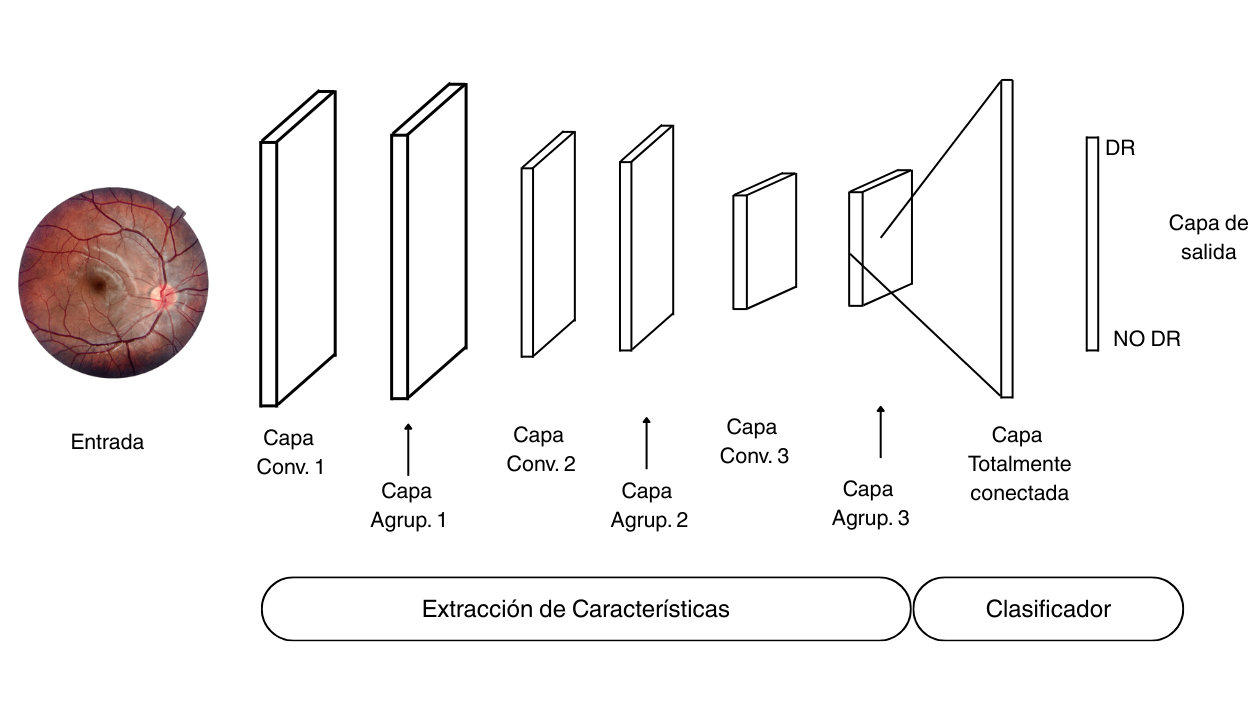
\includegraphics[width=1\textwidth]{imágenes/marco teórico/cnn.png}
	\caption*{\textit{Fuente: Adaptado de arquitecturas CNN estándar}}
\end{figure}

\textbf{Capa convolucional:} Es la primera capa de una red convolucional y su 
componente fundamental: se encarga de extraer la información relevante de la imagen.
Internamente, esta capa está formada por varios filtros de tamaño  $M \times N$
que se deslizan sobre la imagen de entrada hasta recorrerla toda. En cada desplazamiento, 
se calcula el producto punto entre los valores del filtro y los de la región correspondiente
de la imagen. Con estos resultados se construye el mapa de características. Estos mapas revelan
patrones locales como bordes y esquinas, y se utilizan como entrada para capas posteriores, 
que aprenden rasgos más complejos \myfootcite{purwono2022understanding}.

\begin{figure}[H]
	\centering
	\caption{Ejemplo de operación de convolución utilizando un paso de 1 con un
kernel de $3 \times 3$}
	\label{fig:convolution}
	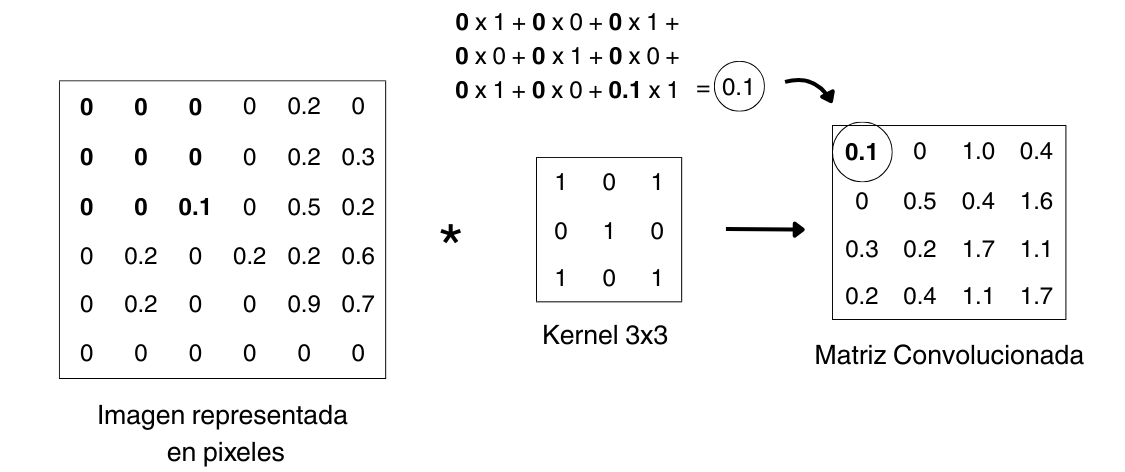
\includegraphics[width=1\textwidth]{imágenes/marco teórico/capa_convolucional.png}
	\caption*{\textit{Fuente: Adaptado de operaciones estándar de CNN}}
\end{figure}

\textbf{Función de activación:} Se aplica una función de activación después de cada
operación de convolución. Esta función ayuda a la red a aprender relaciones no lineales
entre las características de la imagen, lo que hace la red más robusta para identificar
distintos patrones. También ayuda a mitigar el problema de desvanecimiento de gradiente.
Las funciones de activación más comunes incluyen ReLU (Rectified Linear Unit), Sigmoid y
Tanh.

\textbf{Capa de agrupamiento:} La capa de agrupación (también llamada pooling) va después
de una capa de convolución, y su propósito es reducir el tamaño espacial del mapa de
características, es decir, su ancho y alto \myfootcite{akgul2024pooling}. Este proceso
disminuye el costo computacional y ayuda a condensar la información local. Las
operaciones de agrupación se aplican a secciones del mapa de características y producen
una versión reducida que conserva lo más importante. Las variantes más usadas son:

\begin{itemize}
    \item \textbf{Max pooling:} para cada sección, selecciona el valor más alto.
    \item \textbf{Average pooling:} calcula la media de los valores en la sección.
    \item \textbf{Min pooling:} selecciona el valor más bajo en cada sección.
\end{itemize}

\begin{figure}[H]
	\centering
	\caption{Ejemplo de max-pooling con un paso de 2 utilizando un filtro de $2
\times 2$}
	\label{fig:maxpooling}
	
\includegraphics[width=0.9\textwidth]{imágenes/marco
teórico/capa_agrupamiento.png}
	\caption*{\textit{Fuente: Adaptado de operaciones estándar de pooling}}
\end{figure}

\textbf{Capa Multi-Head Attention:} Este tipo de bloques fueron introducidos por primera
vez en la arquitectura de transformers \myfootcite{vaswani2017attention}. En esencia, son
un mecanismo que permite a un modelo de IA enfocarse en diferentes partes de una
secuencia de datos y analizar las partes más determinantes de la misma. Estos bloques se
componen de varias "cabezas de atención", por lo que es posible observar los datos desde
múltiples perspectivas. Cada cabeza de atención trabaja con tres elementos principales: Q
(queries), K (keys) y V (values), que son representaciones diferentes de la misma
información de entrada.

En visión computacional, la atención se ha usado de dos maneras complementarias: como
sustituto completo de las convoluciones en arquitecturas tipo ViT (Vision Transformer)
para procesar secuencias de parches, y como complemento de redes convolucionales,
concatenando o integrando mapas de características de atención con los mapas
convolucionales para incorporar contexto no local. En particular, trabajos que integran
atención con CNNs han mostrado mejoras consistentes en clasificación y detección, incluso
en arquitecturas diseñadas para dispositivos móviles \myfootcite{dosovitskiy2020image}.

\textbf{Capa GaussianNoise:} Este tipo de capas aplican durante el entrenamiento una
perturbación aditiva. En términos generales, cada valor de la activación de la capa
recibe ruido gaussiano aleatorio durante la fase de entrenamiento y la capa queda
inactiva durante la inferencia. Esta acción puede interpretarse como una forma de aumento
estocástico aplicado a las características internas de la red y como un regularizador que
evita el sobreajuste al exponer al modelo a versiones ligeramente corruptas de las
representaciones aprendidas. En redes con backbones preentrenados, las capas añadidas
para clasificación suelen contener muchos parámetros nuevos y son especialmente propensas
a sobreajustarse cuando los datos etiquetados disponibles son limitados. Introducir ruido
gaussiano sobre el mapa de características sirve para forzar a que el clasificador
aprenda patrones robustos y no dependientes de valores exactos de activación, y para
simular variabilidad propia de la adquisición de imágenes (ruido del sensor, diferencias
de iluminación o preprocesado). Estudios empíricos en problemas clínicos y de visión han
mostrado mejoras en métricas de generalización y AUC cuando se usa inyección de ruido
\myfootcite{zur2009noise}.

\textbf{Capa completamente conectada:} La capa completamente conectada (FC) está formada
por pesos, sesgos y neuronas. Actúa como un puente que conecta las neuronas que están
presentes entre las capas ocultas y las capas de salida. Estas capas se colocan solo unas
pocas capas antes de la capa de salida. El mapa de características de la capa anterior se
aplana para crear un único vector de características largo. El vector aplanado se pasa a
otras capas completamente conectadas en las que se realizan muchas operaciones
matemáticas. El proceso de clasificación comienza en esta etapa. La
Figura~\ref{fig:flattening} muestra un ejemplo de proceso de aplanamiento que convierte
las características en una única dimensión.

\begin{figure}[H]
    \centering
    \caption{Proceso de Aplanamiento (Flattening) de un Mapa de Características}
    \label{fig:flattening}
    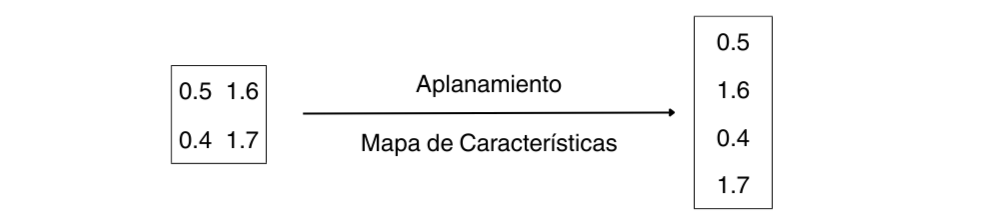
\includegraphics[width=1\textwidth]{imágenes/marco teórico/aplanamiento.png}
    \caption*{\textit{Fuente: Elaboración propia}}
\end{figure}

\subsection{SOBREAJUSTE Y REGULARIZACIÓN}

El sobreajuste (overfitting) es un problema habitual en los modelos de aprendizaje
automático. Ocurre cuando el modelo aprende demasiado los datos de entrenamiento,
incluyendo su ruido y sus valores atípicos, lo que se conoce como "aprendizaje de
memoria". Un aprendizaje de este tipo conduce a un modelo que funciona bien con los datos
de entrenamiento, pero mal con nuevos datos no vistos. Por el contrario, el subajuste
(underfitting) ocurre cuando el modelo es demasiado simple para capturar los patrones
subyacentes en los datos.

\begin{figure}[H]
	\centering
	\caption{Ilustración de subajuste, ajuste adecuado y sobreajuste}
	\label{fig:overfitting}
	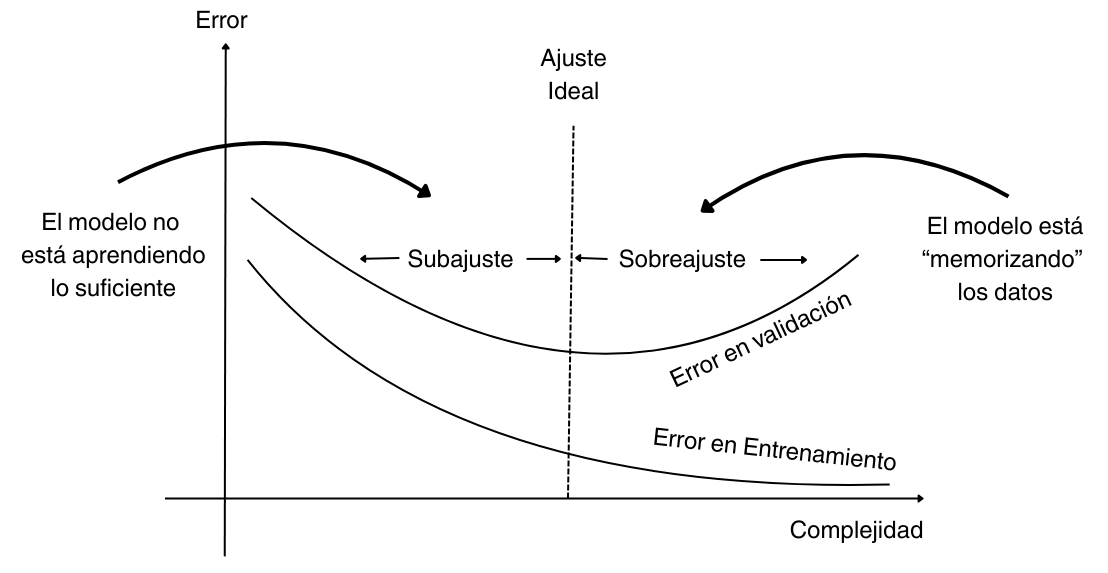
\includegraphics[width=1\textwidth]{imágenes/marco teórico/sobreajuste.png}
	\caption*{\textit{Fuente: Adaptado de conceptos estándar de machine learning}}
\end{figure}

Los modelos de aprendizaje profundo, especialmente las redes neuronales convolucionales
(CNN), son especialmente susceptibles al sobreajuste debido a su alta capacidad y su
habilidad para aprender patrones detallados en datos a gran escala. Existen varias
técnicas de regularización para mitigar el sobreajuste en las CNN. Entre las más comunes
encontramos:

\textbf{Dropout (Abandono):} Esta técnica se basa en desactivar aleatoriamente una
proporción de neuronas durante el entrenamiento, lo que obliga a la red a no depender
excesivamente de neuronas específicas y promueve una representación más robusta de los
datos \myfootcite{garbin2020dropout}. Típicamente, el porcentaje que se desactiva suele
variar entre 0.2 y 0.5. Durante el entrenamiento, las conexiones de las neuronas
desactivadas se eliminan temporalmente, lo que resulta en una red más ligera en cada paso
de entrenamiento. La implementación de esta técnica ha mostrado ser particularmente
efectiva en redes densamente conectadas para mejorar la generalización.

\textbf{Normalización por lotes (Batch Normalization):} El sobreajuste se reduce en
cierta medida normalizando la capa de entrada mediante el ajuste y la escala de las
activaciones. Este enfoque también se utiliza para acelerar y estabilizar el proceso de
entrenamiento al reducir la covarianza interna del modelo.

\textbf{Capas de agrupamiento (Pooling):} Estas capas pueden utilizarse para reducir las
dimensiones espaciales de la imagen de entrada y proporcionar al modelo una forma
abstracta de representación, reduciendo así la posibilidad de sobreajuste al disminuir el
número de parámetros.

\textbf{Parada Anticipada (Early Stopping):} Esta técnica consiste en monitorear el
rendimiento del modelo en un conjunto de validación durante el proceso de entrenamiento y
detenerlo cuando dicho rendimiento deja de mejorar. Así se evita que el modelo se ajuste
demasiado a los datos de entrenamiento y pierda capacidad de generalización. Este método
ha sido probado en distintas investigaciones \myfootcite{brownlee2018gentle}, donde se
demuestra que el early stopping puede reducir el sobreajuste y mejorar la generalización
de las redes neuronales profundas.

\textbf{Inyección de ruido:} Este proceso consiste en añadir ruido a las entradas o a las
salidas de las capas ocultas durante el entrenamiento para hacer más robusto el modelo e
impedir que generalice débilmente.

\textbf{Regularización L1 y L2:} Las técnicas de regularización L1 y L2 consisten en
agregar un término de penalización a la función de pérdida para evitar el sobreajuste.

La regularización L1 (Lasso) añade una penalización proporcional a la suma de los
valores absolutos de los pesos:

\begin{equation}
L_{total} = L_{original} + \lambda \sum_{i} |w_i|
\end{equation}

Esta penalización tiende a llevar los pesos hacia cero, lo que produce modelos dispersos
(\textit{sparse}) y facilita la selección automática de características al eliminar
aquellas menos relevantes.

Por su parte, la regularización L2 (Ridge) añade una penalización proporcional a la
suma de los cuadrados de los pesos:

\begin{equation}
L_{total} = L_{original} + \lambda \sum_{i} w_i^2
\end{equation}

A diferencia de L1, esta técnica reduce la magnitud de los pesos sin llevarlos
exactamente a cero, lo que contribuye a una mayor estabilidad numérica y distribuye
el peso entre características correlacionadas. En ambos casos, $\lambda$ es el hiperparámetro que controla la magnitud de la
penalización. En \myfootcite{kukavcka2017regularization} se presenta una taxonomía
de métodos de regularización en el aprendizaje profundo, destacando la efectividad
de estas técnicas en la mejora de la capacidad de generalización de las redes neuronales.

\textbf{Aumento de datos (Data Augmentation):} Es el proceso de aumentar artificialmente
el tamaño y la diversidad del conjunto de datos de entrenamiento mediante la aplicación
de transformaciones aleatorias, como rotación, escalado, volteo o recorte, a las imágenes
de entrada. Esta técnica es especialmente útil en dominios donde obtener datos
etiquetados es costoso, como en imágenes médicas.

\subsection{APRENDIZAJE POR TRANSFERENCIA}

El aprendizaje por transferencia es un enfoque avanzado dentro del campo del aprendizaje
automático que ha ganado considerable popularidad, especialmente en aplicaciones de
aprendizaje profundo. En este método, un modelo previamente entrenado para realizar una
tarea específica se reutiliza como punto de partida para entrenar un segundo modelo en
una tarea relacionada. Este enfoque es comúnmente utilizado en arquitecturas de redes
neuronales profundas, donde los pesos y parámetros de un modelo previamente entrenado se
transfieren para ser utilizados en un nuevo contexto, lo que permite acelerar el proceso
de entrenamiento y mejorar los resultados en tareas similares.

El aprendizaje por transferencia ofrece múltiples ventajas significativas. Entre ellas
destaca una reducción considerable del tiempo de entrenamiento, ya que al aprovechar
modelos preentrenados que ya han aprendido patrones y características en conjuntos de
datos extensos y generales, se evita entrenar desde cero, lo cual es especialmente
valioso cuando se dispone de datos limitados o se busca reducir costos computacionales
\myfootcite{tan2018survey}. Además, esta técnica permite lograr una mayor precisión y
eficiencia en tareas complejas, como clasificación de imágenes o procesamiento de
lenguaje natural, mediante el ajuste selectivo de capas específicas en lugar de entrenar
toda la red neuronal desde cero \myfootcite{zhuang2020comprehensive}. Por último, el
aprendizaje por transferencia mejora el rendimiento con menos datos, pues al reutilizar
conocimientos adquiridos previamente en conjuntos grandes y diversos, el modelo puede
generalizar mejor incluso con volúmenes reducidos de datos, optimizando así su capacidad
de predicción \myfootcite{weiss2016survey}.

\textbf{Modelo fuente:} Es el modelo previamente entrenado que se selecciona de un
conjunto de modelos candidatos. Este modelo ya ha sido entrenado en un conjunto de datos
grande y general, como ImageNet, y ha aprendido a reconocer patrones y características en
los datos. El modelo fuente proporciona una base sólida que el nuevo modelo puede
aprovechar.

\textbf{Modelo de reutilización:} Una vez que se ha elegido el modelo fuente, este se
utiliza como punto de partida para un nuevo modelo que debe ser entrenado en una tarea
diferente pero relacionada. Dependiendo de los requisitos del problema y de las técnicas
utilizadas, se puede optar por reutilizar todo el modelo o solo ciertas partes, como las
capas de la red que han aprendido características generales (por ejemplo, bordes y
texturas en el caso de imágenes).

\textbf{Ajuste fino (Fine-tuning):} Después de reutilizar el modelo entrenado, es posible
que sea necesario ajustar o afinar ciertas partes del modelo para que se adapte mejor a
los nuevos datos y tareas. Este proceso implica ajustar los pesos del modelo para que se
especialice en las etiquetas de salida del nuevo conjunto de datos, lo cual se logra a
través de una cantidad reducida de entrenamiento adicional.



\section{ARQUITECTURAS DE REDES NEURONALES CONVOLUCIONALES UTILIZADAS}

La retinopatía diabética es una enfermedad ocular compleja y de diagnóstico desafiante,
que requiere una alta precisión en la detección de cambios sutiles en las imágenes del
fondo de ojo. Los modelos preentrenados, especialmente aquellos basados en arquitecturas
profundas de redes neuronales convolucionales (CNN), han demostrado ser eficaces en
tareas de procesamiento de imágenes. Dado que estos modelos han aprendido a identificar
patrones de alto nivel en datos visuales durante su entrenamiento previo, pueden
transferir ese conocimiento a la tarea de identificación de lesiones retinianas, como
microaneurismas, exudados y hemorragias, mejorando la exactitud del diagnóstico.

A continuación se detallan las cuatro arquitecturas de CNN seleccionadas para este
trabajo experimental, elegidas por sus características complementarias en términos de
complejidad, eficiencia computacional y capacidad de generalización.

\subsection{MOBILENETV2}

MobileNetV2 es una red neuronal convolucional optimizada para dispositivos móviles y
aplicaciones con recursos limitados. Fue presentada por Google en 2018 por Mark Sandler,
Andrew Howard, Menglong Zhu y colaboradores \myfootcite{sandler2018mobilenetv2}.
MobileNetV2 está diseñada para ser eficiente tanto en términos de número de parámetros
como en cálculos requeridos, lo que la hace adecuada para dispositivos con recursos
limitados. La principal novedad de MobileNetV2 respecto a la versión anterior
(MobileNetV1) es el uso de bloques residuales invertidos y cuellos de botella lineales,
que permiten que la red mantenga un alto rendimiento mientras reduce la complejidad
computacional.

Al igual que en MobileNetV1, esta red utiliza convoluciones separables en profundidad
(depthwise separable convolutions). Este tipo de convolución separa el filtrado en dos
pasos: una convolución de filtro por canal y una convolución $1 \times 1$ para combinar
los resultados. Este enfoque reduce la cantidad de cálculos y parámetros respecto a las
convoluciones tradicionales.

El corazón de esta arquitectura son los bloques residuales invertidos. En estos, las
características primero se expanden a una dimensión mayor y posteriormente se procesan
mediante una convolución separable en profundidad. Por último, las características se
proyectan de nuevo a una dimensión más baja mediante una convolución de $1 \times 1$.

Otro aspecto único de MobileNetV2 es el uso de cuellos de botella lineales. Esto
significa que después de la expansión de las características, la proyección de vuelta a
un espacio de menor dimensión se realiza sin activaciones no lineales. Este enfoque ayuda
a mantener la representación de características más eficiente, lo que se traduce en una
mayor precisión y velocidad de la red en comparación con las redes tradicionales que usan
activaciones no lineales después de la reducción de dimensiones.

\begin{figure}[H]
	\centering
	\caption{Arquitectura de MobileNetV2 mostrando bloques residuales invertidos}
	\label{fig:mobilenetv2}
	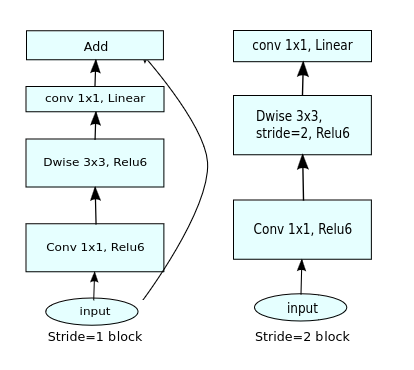
\includegraphics[width=0.8\textwidth]{imágenes/metodología/ArqMobilNetV2.png}
	\caption*{\textit{Fuente: Sandler et al. (2018)}}
\end{figure}

En general, la arquitectura de MobileNetV2 se compone de una serie de bloques residuales
invertidos que incluyen: expansión, la cual es una convolución de $1 \times 1$ que
incrementa la dimensión de características; convolución por profundidad, que es una
convolución separable en profundidad que aplica filtros de tamaño $3 \times 3$; y una
proyección, que es una convolución de $1 \times 1$ que reduce la dimensión de las
características a su tamaño original.

\subsection{RESNET50V2}

ResNet50V2 es una variante mejorada de la arquitectura ResNet (Red Residual) original,
introducida con el objetivo de optimizar el flujo del gradiente durante el entrenamiento
y, en consecuencia, mejorar la capacidad de generalización y rendimiento. Esta versión
fue presentada en el trabajo de Kaiming He, Xiangyu Zhang, Shaoqing Ren y Jian Sun
\myfootcite{he2016identity}.

El núcleo de ResNet, y por ende de ResNet50V2, son los llamados bloques residuales. Estos
bloques incluyen conexiones de salto (skip connections) que permiten que el gradiente
fluya más fácilmente hacia las capas iniciales durante el entrenamiento, mitigando el
problema del desvanecimiento del gradiente en redes muy profundas. En la versión V2, la
principal diferencia respecto a la original (V1) es que se reorganizan las operaciones en
el bloque residual, además de que se incluyen mapeos de identidad mejorados y una mejor
normalización \myfootcite{he2016identity}.

Mientras que en ResNetV1 se utiliza una estructura del tipo convolución seguida de Batch
Normalization y Activación ReLU, en ResNetV2 se antecede la normalización y la activación
antes de la convolución, siguiendo un enfoque de pre-activación. Este cambio en el orden
de las operaciones mejora el flujo de gradientes y facilita el entrenamiento de redes más
profundas.

\begin{figure}[H]
	\centering
	\caption{Arquitectura de ResNet50V2 con bloques residuales mejorados}
	\label{fig:resnet50v2}
	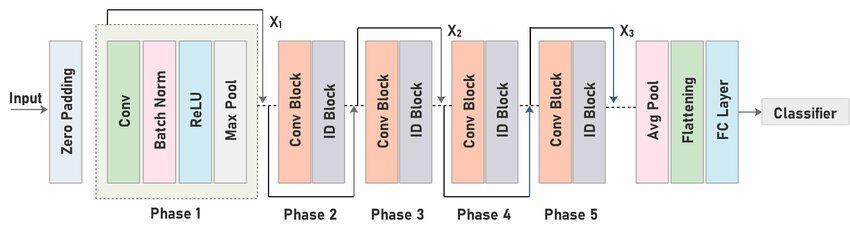
\includegraphics[width=1\textwidth]{imágenes/metodología/arqResNet50v2.jpg}
	\caption*{\textit{Fuente: He et al. (2016)}}
\end{figure}

La arquitectura de esta red está compuesta por 50 capas profundas, organizadas en
distintos bloques residuales con diferentes configuraciones de filtros y tamaños. Cada
bloque residual en ResNet50V2 utiliza una estructura bottleneck, que consiste en tres
capas convolucionales: $1 \times 1$, $3 \times 3$ y $1 \times 1$, lo que permite una
reducción y expansión eficiente de las dimensiones de las características.

\subsection{INCEPTIONV3}

InceptionV3 es una arquitectura de red neuronal convolucional desarrollada para tareas de
clasificación de imágenes, reconocida por su eficiencia y precisión. Es una evolución de
las versiones anteriores de la familia Inception, introducida por Christian Szegedy y
colaboradores de Google, introduciendo mejoras significativas en el procesamiento de
características y la reducción de la complejidad computacional
\myfootcite{szegedy2016rethinking}. La arquitectura busca maximizar la eficiencia del
modelo mediante la optimización de las operaciones convolucionales.

El componente principal de esta red son los módulos Inception. Estos combinan múltiples
tipos de convoluciones y operaciones de pooling en paralelo dentro de una misma capa, lo
que permite a la red capturar información a diferentes escalas y contextos espaciales de
forma simultánea. En esta red, los módulos se optimizan mediante la factorización de
convoluciones más grandes en secuencias de convoluciones más pequeñas y eficientes. Por
ejemplo, una convolución de $5 \times 5$ puede descomponerse en dos convoluciones de $3
\times 3$, reduciendo así el número de parámetros y el costo computacional.

Además, InceptionV3 incorpora capas de reducción de dimensionalidad utilizando
convoluciones $1 \times 1$. Estas capas ayudan a disminuir la dimensionalidad de las
características antes de aplicar convoluciones más costosas, lo que mejora la eficiencia.
También se utiliza la normalización por lotes después de cada convolución, lo que
estabiliza y acelera el entrenamiento al normalizar las activaciones de cada capa.

Otra de las características de la arquitectura de InceptionV3 es el uso de convoluciones
asimétricas para capturar características espaciales de manera más eficiente. Estas
convoluciones permiten que la red mantenga una alta capacidad de representación sin
incrementar significativamente el número de parámetros. Además, para mejorar la
propagación de la información de las etiquetas en las capas inferiores de la red y
mitigar el problema del desvanecimiento del gradiente, InceptionV3 utiliza clasificadores
auxiliares. Estos clasificadores adicionales actúan como regularizadores durante el
entrenamiento, mejorando la convergencia y la precisión del modelo.

\begin{figure}[H]
	\centering
	\caption{Arquitectura de InceptionV3 con módulos Inception paralelos}
	\label{fig:inceptionv3}
	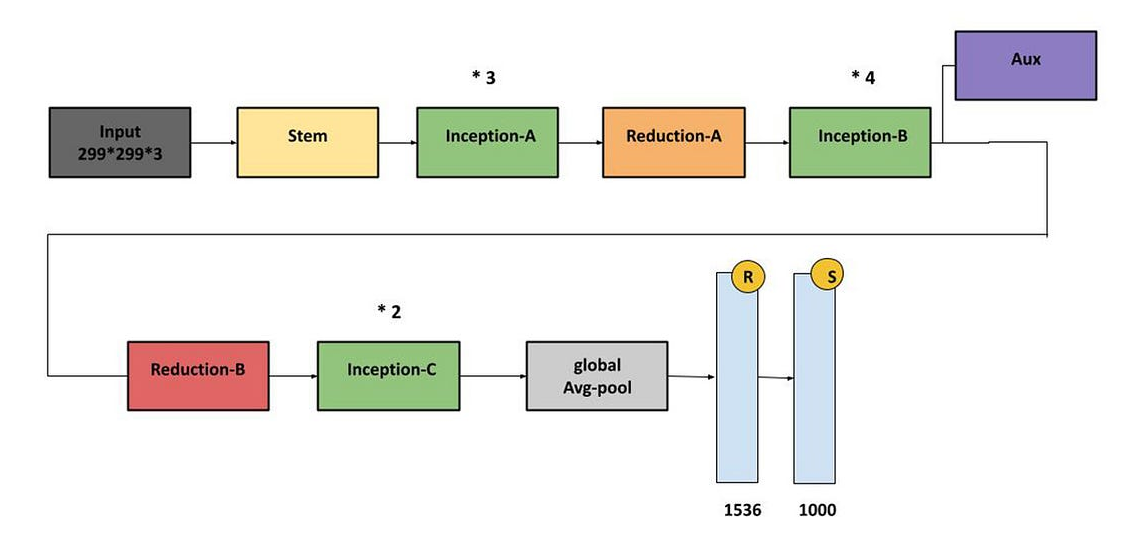
\includegraphics[width=1\textwidth]{imágenes/metodología/Arqinceptionv3.png}
	\caption*{\textit{Fuente: Szegedy et al. (2016)}}
\end{figure}

En general, la arquitectura de InceptionV3 está compuesta por una capa de entrada,
seguida de módulos Inception con factorización de convoluciones y reducción de
dimensionalidad. Por último se aplica una capa de Global Average Pooling seguida de capas
completamente conectadas para la clasificación final.

\subsection{VGG19}

La arquitectura VGG19 pertenece a la familia de redes VGG (Visual Geometry Group) y fue
desarrollada con el objetivo de investigar la relación entre la profundidad de las redes
neuronales y su rendimiento. Esta red convolucional profunda fue introducida por Karen
Simonyan y Andrew Zisserman de la Universidad de Oxford y diseñada específicamente para
tareas de clasificación de imágenes. VGG19 se caracteriza por tener 19 capas en total: 16
de ellas son convolucionales y las 3 restantes son capas completamente conectadas. A
pesar de su complejidad, la arquitectura de VGG19 se distingue por su simplicidad y su
diseño sistemático, en el que se emplean filtros pequeños de $3 \times 3$ píxeles a lo
largo de las capas convolucionales.

La estructura de VGG19 está organizada en bloques secuenciales de capas convolucionales,
seguidos de capas de pooling y finalizando con capas totalmente conectadas. Cada bloque
convolucional consta de entre 2 y 4 capas convolucionales, todas utilizando filtros de
tamaño $3 \times 3$, con un stride de 1 y un padding de 1. Esta configuración permite
mantener el tamaño espacial de las características durante el proceso de extracción, lo
que ayuda a preservar la resolución de las imágenes a medida que se procesan a través de
la red.

Uno de los aspectos clave de VGG19 es su uso de filtros pequeños ($3 \times 3$), lo que
facilita una mayor capacidad de aprendizaje y un control más fino sobre las
características extraídas en cada capa. Además, la red utiliza capas de max pooling para
reducir la dimensionalidad y la complejidad computacional sin perder información
importante.

VGG19 ha sido una de las arquitecturas más influyentes en el campo de la visión por
computadora debido a su rendimiento sobresaliente en tareas de clasificación de imágenes,
como se demostró en la competencia ImageNet. La red también ha sido utilizada como modelo
base en diversos problemas relacionados con el procesamiento de imágenes, adaptándose
fácilmente a tareas como detección de objetos, segmentación y, en el caso de la
retinopatía diabética, clasificación de imágenes médicas.

\begin{figure}[H]
	\centering
	\caption{Arquitectura de VGG19 con bloques convolucionales secuenciales}
	\label{fig:vgg19}
	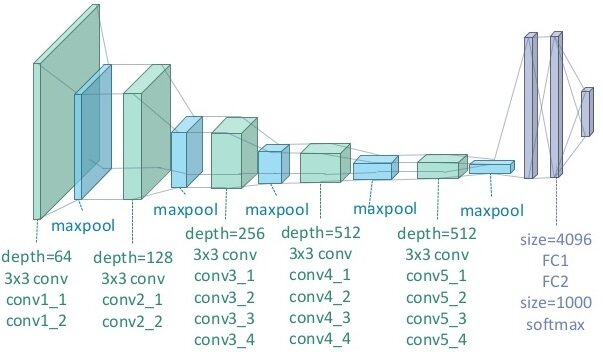
\includegraphics[width=1\textwidth]{imágenes/metodología/arqVgg19.jpg}
	\caption*{\textit{Fuente: Simonyan \& Zisserman (2014)}}
\end{figure}

\subsection{Comparación de arquitecturas}

La Tabla~\ref{tab:comparacion-arquitecturas} presenta una comparación cuantitativa de las
cuatro arquitecturas seleccionadas, considerando aspectos clave para su aplicación en
clasificación de imágenes médicas.

\begin{table}[H]
\centering
\renewcommand{\arraystretch}{1.3}
\caption{Comparación de arquitecturas CNN utilizadas en este trabajo}
\label{tab:comparacion-arquitecturas}
\begin{tabularx}{\textwidth}{l X c c X}
\hline
\textbf{Arquitectura} & \textbf{Características distintivas} & \textbf{Capas} &
\textbf{Parámetros} & \textbf{Ventaja principal} \\ \hline
MobileNetV2 & Bloques residuales invertidos, convoluciones separables & 53 & $\sim$3.5M &
Eficiencia computacional \\
ResNet50V2 & Conexiones residuales con pre-activación & 50 & $\sim$25M & Entrenamiento de
redes profundas \\
InceptionV3 & Módulos Inception paralelos, factorización & 48 & $\sim$24M & Captura
multiescala \\
VGG19 & Arquitectura simple y profunda con filtros 3x3 & 19 & $\sim$144M & Simplicidad
arquitectónica \\ \hline
\end{tabularx}
\end{table}

Cada una de estas arquitecturas aporta características complementarias al estudio
experimental. MobileNetV2 ofrece eficiencia computacional crucial para aplicaciones en
recursos limitados; ResNet50V2 permite entrenar modelos muy profundos sin degradación de
rendimiento; InceptionV3 captura información a múltiples escalas mediante sus módulos
paralelos; y VGG19, a pesar de su mayor cantidad de parámetros, ofrece una arquitectura
simple que ha demostrado efectividad en tareas de clasificación de imágenes médicas.
 % Fundamentos teóricos
\chapter{TRABAJOS PREVIOS} \label{chap:trabajos-previos}

En los últimos años, las técnicas de aprendizaje profundo han demostrado un rendimiento
excepcional en numerosas tareas que van desde el reconocimiento de objetos hasta el
procesamiento del lenguaje natural. El uso de técnicas de aprendizaje profundo,
específicamente redes neuronales convolucionales (CNN), ha demostrado resultados
prometedores en la detección automática de RD a través del análisis de imágenes del fondo
de ojo. Dentro de este contexto, se incluyen varios enfoques que han contribuido en este
campo de investigación.

\section{Enfoques con CNN personalizadas}

Este problema se ha abordado de distintas formas, planteándose distintas soluciones. En
general, podemos ver en la literatura una preponderancia de la implementación de modelos
previamente entrenados. Esto toma sentido cuando consideramos el costo de entrenamiento
que tienen este tipo de modelos que se alimentan de cientos de miles de imágenes; solo
pocos sectores de la industria tienen los recursos necesarios para llevar a cabo estos
desarrollos. Muchos de los artículos recopilatorios encargados de comparar soluciones
frente a la clasificación de la RD se encargan, en última instancia, de comparar la
efectividad de distintos modelos preentrenados para la clasificación de la RD
\myfootcite{bala2024comparative}, donde se comparan ocho de los modelos preentrenados más
utilizados desde 2011 hasta 2022.

En algunas investigaciones se observa un enfoque común: la personalización de un modelo
de red neuronal convolucional (CNN) para abordar la detección automatizada de retinopatía
diabética (RD). Esta estrategia implica modificar la arquitectura o los parámetros de un
modelo CNN tradicional y mejorarlo en la tarea específica de la detección de RD. En este
contexto, se han explorado diversas estrategias para mejorar la precisión y eficiencia de
la detección de RD a partir de imágenes del fondo de la retina. Por ejemplo, se han
aplicado etapas de preprocesamiento como escalado, recorte y ecualización adaptativa del
histograma con limitación de contraste (CLAHE) para mejorar la calidad de las imágenes
\myfootcite{tabtaba2024diabetic}.

Además, se han utilizado técnicas de aumento de datos mediante redes generativas
adversariales (GAN) para enriquecer el conjunto de datos de entrenamiento. Otros trabajos
han introducido variantes personalizadas de CNN, como la Red Neuronal Convolucional
Dilatada Multiescala Híbrida en Cascada (HCMD-CNN) \myfootcite{gayathri2020lightweight},
que integra la Red de Atención Residual (RAN) y MobileNet, optimizando sus parámetros
para lograr un mejor rendimiento en la detección de RD. Otros enfoques han empleado
métodos de extracción de características mediante CNN, cuyas salidas se utilizan como
entrada para diferentes clasificadores de aprendizaje automático
\myfootcite{li2019computer} \myfootcite{gayathri2021diabetic}, como Support Vector
Machine, AdaBoost, Naive Bayes, Random Forest y J48.

\section{Enfoques con arquitecturas preentrenadas}

Últimamente se han desarrollado otras aproximaciones que aprovechan arquitecturas
preentrenadas en el ámbito de la detección y clasificación de retinopatía diabética (RD)
en imágenes del fondo de ojo. Estos enfoques abarcan una variedad de modelos de
aprendizaje profundo, tales como VGG16, InceptionResNetv2, Inceptionv3, DenseNet121,
MobileNetV2, Xception y YOLOv3, los cuales se han utilizado para extraer características
y llevar a cabo tareas de clasificación y detección.

Por ejemplo, un estudio implementó una red neuronal convolucional (CNN) utilizando VGG16
para la extracción de características de imágenes de retina y la técnica de sobremuestreo
de minoría sintética (SMOTE) para manejar el desequilibrio de clases en el conjunto de
datos \myfootcite{mustafa2024rapid}, logrando una precisión del 93.94\% durante la fase
de entrenamiento y del 88.19\% durante la validación.

Otro enfoque consistió en dos modelos basados en aprendizaje profundo: CNN512, que
clasificó imágenes completas en estadios de RD con una precisión del 88.6\%, y un modelo
YOLOv3 adaptado para detectar y localizar lesiones de DR, alcanzando un mAP de 0.216 en
la localización de lesiones \myfootcite{alyoubi2021diabetic}. Estos modelos se fusionaron
para clasificar imágenes de RD y localizar lesiones, obteniendo una precisión del 89\%
con sensibilidad del 89\% y especificidad del 97.3\%.

Además, se ha explorado el aprendizaje por transferencia utilizando modelos preexistentes
como InceptionResNetv2 e Inceptionv3, junto con un nuevo modelo DiaCNN, para la
clasificación de enfermedades oculares en el conjunto de datos ODIR
\myfootcite{shoaib2024deep}. Estos modelos alcanzaron impresionantes niveles de
precisión, llegando hasta el 99.7\% en algunas pruebas.

Asimismo, se ha abordado la detección automática de vasos sanguíneos retinianos
utilizando modelos como ResNet34, InceptionV3 y VGG16, y se han propuesto enfoques
multinivel \myfootcite{beghriche2023multi} para mejorar la clasificación binaria y
multiclase de imágenes de RD \myfootcite{vij2024hybrid}, logrando una precisión del
96.50\% en la clasificación binaria y una kappa ponderada cuadrática del 93.00\% en la
clasificación por etapas. Estos avances muestran mejoras significativas en precisión y
generalización, con resultados que superan a los métodos tradicionales y a los trabajos
previos en la literatura.

\section{Enfoques con modificaciones arquitectónicas innovadoras}

Por otra parte, existen otros trabajos en la literatura que han optado por realizar
modificaciones sustanciales a las arquitecturas CNN para obtener un mejor desempeño. Se
han propuesto varias técnicas innovadoras para mejorar el rendimiento y la eficiencia del
aprendizaje profundo en la detección y clasificación de retinopatía diabética (RD)
\myfootcite{patil2023study}.

Un estudio aborda el aprendizaje profundo distribuido (DDL) para entrenar modelos de DL
de manera rápida, utilizando dos GPU y analizando el rendimiento del canal de paralelismo
en DDL, logrando una puntuación F1 de validación de 0.834 en la clasificación de RD. Otro
enfoque se centra en la diversidad de los conjuntos de datos de entrenamiento mediante la
manipulación de datos de entrada, mejorando así el rendimiento de la clasificación
\myfootcite{patil2022pipeline}.

Además, se propone un enfoque bioinspirado en la metaplasticidad sináptica, que se
incorpora en redes neuronales convolucionales para fortalecer las ocurrencias menos
comunes durante el aprendizaje \myfootcite{vives2021diabetic}. Este método mejora tanto
la tasa de aprendizaje como la precisión, superando a otros métodos de la literatura
actual incluso con conjuntos de datos más pequeños, con resultados destacados en la
arquitectura InceptionV3.

\section{Limitaciones y brechas de investigación}

A pesar del avance significativo en el uso de técnicas de aprendizaje profundo para la
detección de RD a partir de imágenes del fondo de ojo, aún existen algunas limitaciones
que deben abordarse para garantizar su aplicabilidad en el mundo real y su adopción en la
práctica clínica.

La mayoría de los modelos actuales se entrenan con conjuntos de datos limitados y
específicos, lo que limita su capacidad para generalizar a escenarios del mundo real con
mayor variabilidad en las imágenes del fondo de ojo. En muchos conjuntos de datos, las
imágenes con RD representan una pequeña proporción en comparación con las imágenes
normales. Este desequilibrio de clases puede afectar el rendimiento del modelo, sesgando
la clasificación hacia la clase mayoritaria.

Algunos estudios se enfocan únicamente en la detección de la presencia o ausencia de RD,
sin considerar la clasificación de su gravedad en estadios tempranos, moderados o
severos, lo cual es crucial para la toma de decisiones oportunas en el manejo de la
enfermedad. El ruido, la iluminación inconsistente y el bajo contraste en las imágenes
del fondo de ojo pueden afectar significativamente la precisión de la clasificación. La
implementación de técnicas de preprocesamiento de imágenes robustas es fundamental para
mejorar el rendimiento de los modelos.

Pocos trabajos han explorado sistemáticamente el efecto del procesamiento de canales de
color individuales (rojo, verde, azul) en el desempeño de clasificación de RD, a pesar de
que diferentes canales pueden resaltar lesiones específicas. Además, existe una escasez
de validación externa rigurosa en múltiples datasets con características de adquisición
diferentes, lo cual es esencial para demostrar la capacidad de generalización de los
modelos.

\section{Contribución del presente trabajo}

El empleo de algoritmos de aprendizaje profundo en la detección de RD a partir de
imágenes del fondo de ojo presenta un gran potencial para mejorar la accesibilidad, la
precisión y la eficiencia del tamizaje de esta enfermedad. Sin embargo, es necesario
abordar las limitaciones actuales relacionadas con la generalización de los modelos, el
desequilibrio de clases, la clasificación de la gravedad y el preprocesamiento de
imágenes para garantizar su aplicabilidad en entornos clínicos reales y su adopción como
una herramienta confiable para el diagnóstico y seguimiento de la RD.

El presente trabajo contribuye al estado del arte en los siguientes aspectos:

\begin{itemize}
    \item \textbf{Análisis sistemático de canales de color:} Evaluación comparativa del
desempeño de modelos procesando imágenes RGB completas versus canales individuales (rojo,
verde, azul), identificando el canal más efectivo para clasificación multiclase.

    \item \textbf{Comparación controlada de arquitecturas:} Evaluación sistemática de
cuatro arquitecturas CNN preentrenadas (MobileNetV2, ResNet50V2, InceptionV3, VGG19) bajo
condiciones experimentales idénticas.

    \item \textbf{Validación externa rigurosa:} Evaluación del mejor modelo en tres
datasets externos independientes (MESSIDOR-2, IDRiD, FOSCAL) con diferentes
características de adquisición y distribución de clases.

    \item \textbf{Combinación de técnicas de regularización:} Integración de bloques
Multi-Head Attention, capas GaussianNoise y técnicas tradicionales (Dropout, L2, early
stopping) para mejorar generalización.

    \item \textbf{Enfoque dual de clasificación:} Desarrollo y evaluación tanto de
clasificadores binarios (optimizados para tamizaje) como multiclase (para gradación
clínica), permitiendo su aplicación en diferentes escenarios clínicos.
\end{itemize}
 % Trabajos previos


\chapter{METODOLOGÍA} \label{chap:metodologia}

Este capítulo describe el procedimiento metodológico seguido para desarrollar e 
implementar los modelos de clasificación de retinopatía diabética basados en aprendizaje 
profundo. La metodología se estructura en cinco etapas principales: primero, 
la recopilación y caracterización de conjuntos de datos de imágenes de fondo de ojo; 
segundo, el preprocesamiento y balanceo de datos para optimizar la calidad del 
conjunto de entrenamiento; tercero, la selección de tecnologías y herramientas de 
desarrollo; cuarto, la configuración e implementación de las arquitecturas CNN con 
técnicas de regularización; y finalmente, la definición de métricas de evaluación para 
validar el desempeño de los modelos. La Figura~\ref{fig:metodologia-general} presenta un diagrama que sintetiza el flujo
completo del proceso metodológico implementado.

\begin{figure}[H]
	\centering
	\caption{Estructura metodológica propuesta para la clasificación de retinopatía 
diabética mediante aprendizaje profundo}
	\label{fig:metodologia-general}
	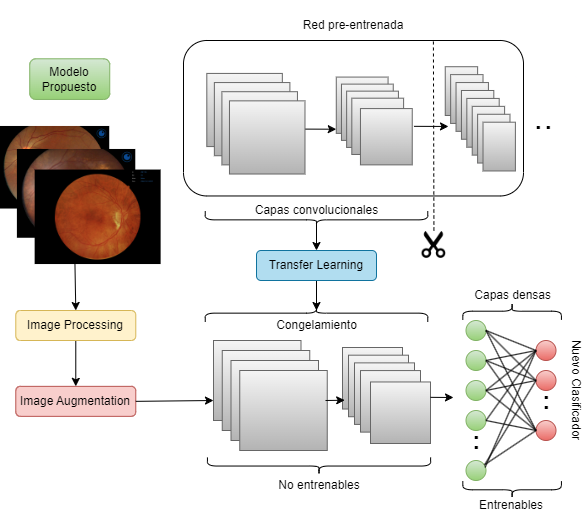
\includegraphics[width=1\textwidth]{imágenes/metodología/MODELO.png}
	\caption*{\textit{Fuente: Elaboración propia}}
\end{figure}

\section{CONJUNTOS DE DATOS} \label{sec:conjuntos-datos}

Una etapa clave en la construcción de una red neuronal convolucional (CNN) es la 
recopilación de datos, ya que el rendimiento del modelo depende en gran medida tanto de 
la calidad como de la diversidad del conjunto utilizado. Para que el entrenamiento sea 
efectivo, las imágenes deben reflejar con precisión las distintas condiciones del 
problema y pueden obtenerse a partir de repositorios públicos, fuentes en línea o 
mediante técnicas de generación artificial. Es esencial que cada imagen esté 
correctamente clasificada según corresponda, ya que una mala etiquetación puede afectar 
negativamente el aprendizaje del modelo. Por ello, es importante realizar una curaduría 
rigurosa del dataset, priorizando imágenes representativas y bien definidas.

En el desarrollo de este proyecto se utilizaron distintos conjuntos de datos para 
garantizar la robustez y generalización del modelo. Inicialmente se exploraron datasets 
disponibles en repositorios públicos, junto con un conjunto de datos de propiedad 
privada. La fase experimental inicial se llevó a cabo con el dataset de Kaggle debido a 
su gran volumen de imágenes. Posteriormente se utilizaron los datasets públicos
MESSIDOR-2, IDRiD y uno privado denominado FOSCAL para evaluar la capacidad de
generalización del modelo final mediante validación externa: el modelo, entrenado
exclusivamente con el dataset de Kaggle, fue evaluado directamente sobre estos tres
conjuntos sin reentrenamiento ni ajuste de pesos.

\subsection{Dataset de Kaggle (Entrenamiento)}

Es el dataset principal que se utilizó para entrenar y validar los modelos
experimentales. Cuenta con un amplio conjunto de datos compuesto por imágenes de retina
en alta resolución, obtenidas a partir del repositorio \textit{Diabetic Retinopathy
Detection 2015}, disponible en la plataforma Kaggle. Las imágenes provienen de EyePACS,
una red de telemedicina para tamizaje de retinopatía diabética que opera principalmente
en centros de atención primaria de California, Estados Unidos
\myfootcite{cuadros2009eyepacs}. Las imágenes fueron capturadas bajo
diversas condiciones y con distintos tipos de cámaras, lo que introduce variabilidad en
aspectos como la resolución, la iluminación y la orientación.

Cada registro corresponde a un paciente, identificándose ambos ojos mediante un nombre de 
archivo que incluye el número de paciente seguido de \enquote{izquierda} o
\enquote{derecha} (por 
ejemplo: \texttt{1\_izquierda.jpg}). Cada imagen fue evaluada por un especialista 
clínico, quien asignó un grado de severidad de retinopatía diabética utilizando una
escala ordinal de 0 a 4: 0, sin retinopatía diabética; 1, leve; 2, moderada; 3, severa;
y 4, retinopatía diabética proliferativa.

La naturaleza heterogénea del conjunto se evidencia en las diferencias anatómicas y de 
orientación presentes en las imágenes: algunas muestran la retina con una disposición 
convencional (mácula a la izquierda y nervio óptico a la derecha en el caso del ojo 
derecho), mientras que otras presentan una orientación invertida, similar a la observada 
a través de un microscopio durante un examen clínico. La orientación puede determinarse a 
partir de la posición relativa entre la mácula y el nervio óptico, así como por la 
presencia de muescas laterales en la imagen.

Es importante señalar que el conjunto contiene ruido, tanto en las imágenes (como 
artefactos, desenfoque, subexposición o sobreexposición), como en las etiquetas, debido a 
la subjetividad inherente a la evaluación clínica. Por esta razón, uno de los retos 
principales de este estudio es desarrollar algoritmos robustos, capaces de enfrentar 
dicha variabilidad y el ruido presente en los datos, asegurando un desempeño confiable en 
escenarios reales de aplicación.

\subsection{MESSIDOR-2 (Validación externa)}

Es una base de datos de imágenes de fondo de ojo diseñada para evaluar algoritmos de
detección de retinopatía diabética, particularmente para la clasificación de casos
referibles. Contiene un total de 1,748 imágenes correspondientes a 874 exámenes de
pacientes, provenientes de tres departamentos de oftalmología en Francia: el Hospital
Universitario de Brest, el Hospital Universitario de Saint-Étienne y el Hôpital
Lariboisière de París \myfootcite{decenciere2014messidor}. Las imágenes fueron
capturadas con cámaras no midriáticas Topcon TRC NW6, NW7 y Nidek AFC-210, con
un campo de visión de 45°. Las imágenes presentan resoluciones variables, típicamente
entre $1440 \times 960$ y $2304 \times 1536$ píxeles, y están centradas en la mácula.

Este conjunto cuenta con: etiquetas de gradación de retinopatía diabética (RD) en una 
escala de 0 a 3; etiquetas de edema macular, validadas por especialistas; y metadatos 
como el diámetro pupilar y la calidad técnica de cada imagen. Gracias a su calidad, 
volumen y amplia adopción en la comunidad científica, MESSIDOR-2 es ampliamente empleado 
como benchmark para evaluar el rendimiento y la generalización de modelos de 
clasificación de RD, especialmente en escenarios de validación externa y estudios 
comparativos.

\subsection{IDRiD (Validación externa)}

El \textit{Indian Diabetic Retinopathy Image Dataset} contiene un total de 516 imágenes 
de retina en alta resolución ($4288 \times 2848$ píxeles), capturadas con una cámara Kowa 
VX-10$\alpha$ con un campo de visión de 50\textdegree, centradas en la mácula. Las 
imágenes provienen de pacientes del Aravind Eye Hospital en India y están acompañadas de 
anotaciones detalladas realizadas por expertos clínicos.

Este conjunto incluye: etiquetas de clasificación de severidad de RD; segmentaciones a 
nivel de píxel para lesiones específicas como microaneurismas, hemorragias, exudados 
duros y blandos; y segmentaciones de estructuras anatómicas como la fóvea y el disco 
óptico. El dataset se divide en un conjunto de entrenamiento con 413 imágenes y un 
conjunto de prueba con 103 imágenes, lo que lo hace especialmente útil tanto para tareas 
de clasificación como de segmentación.

\subsection{FOSCAL (Validación externa)}

El dataset FOSCAL está compuesto por 1,538 imágenes de fondo de ojo, obtenidas gracias al 
Centro de Prevención y Consultoría en Glaucoma de Bucaramanga (Fundación Oftalmológica de 
Santander - FOSCAL). Las imágenes estaban acompañadas de un archivo plano que detalla las 
anomalías presentes, incluyendo el nivel de retinopatía diabética (RD), lo que permitió 
organizarlas con sus respectivas etiquetas.

El proceso de etiquetado fue realizado por especialistas médicos mediante una plataforma 
web diseñada específicamente para la lectura y tamizaje. Esta plataforma incluía 
funcionalidades para descartar imágenes de baja calidad o no evaluables, garantizando así 
la confiabilidad de los datos. Este dataset representa condiciones clínicas locales y fue 
utilizado como validación externa para evaluar el desempeño del modelo en un contexto 
colombiano específico.

\subsection{Distribución de datos}

La Tabla~\ref{tab:distribucion_clases} presenta la distribución de imágenes por clase de 
severidad en cada uno de los datasets utilizados, mostrando la variabilidad en la 
distribución de clases entre diferentes fuentes de datos.

\begin{table}[H]
	\centering
	\renewcommand{\arraystretch}{1.5}
	\caption{Distribución de imágenes por clase de severidad de retinopatía diabética 
en los distintos datasets}
	\label{tab:distribucion_clases}
	\begin{tabularx}{\textwidth}{X c c c c c c c}
		\hline
		\textbf{Dataset} & \textbf{No RD} & \textbf{Leve} & \textbf{Moderada} & 
\textbf{Severa} & \textbf{Prolif.} & \textbf{Total} & \textbf{Uso} \\
		\hline
		Kaggle & 25,810 & 2,443 & 5,292 & 873 & 703 & 35,121 & Entrenamiento \\
		MESSIDOR & 1,017 & 270 & 347 & 114 & --- & 1,748 & Validación ext. \\
		IDRiD & 213 & 117 & 54 & 56 & 76 & 516 & Validación ext. \\
		FOSCAL & 302 & 34 & 23 & 40 & 16 & 415 & Validación ext. \\
		\hline
	\end{tabularx}
	\caption*{\textit{Fuente: Elaboración propia}}
\end{table}

Como puede observarse en la Tabla~\ref{tab:distribucion_clases}, el desbalance hacia la
clase No RD no es exclusivo del dataset de Kaggle (73.5\%): FOSCAL presenta una
proporción similar (72.8\%), mientras que IDRiD resulta considerablemente más balanceado
(41.3\% de la clase mayoritaria). MESSIDOR, por su parte, no incluye casos etiquetados
como retinopatía proliferativa, lo que ilustra la heterogeneidad en los criterios de
recolección y etiquetado entre los datasets externos utilizados para la validación, un
factor que se retoma en la discusión de la capacidad de generalización del modelo
(Capítulo~\ref{chap:discusion}).

\subsection{División de datos para entrenamiento y validación} \label{subsec:division-datos}

El dataset de Kaggle se dividió en tres subconjuntos siguiendo una estrategia de
partición estratificada. Esta elección responde directamente al marcado desbalance de
clases del conjunto original, descrito en la Sección~\ref{subsec:balanceo-clases}, donde
la clase 0 (sin RD) representa aproximadamente el 73\% de las imágenes frente a apenas un
2\% de la clase 4 (RD proliferativa): una partición completamente aleatoria podría, por
azar, generar subconjuntos con proporciones de clase distintas entre sí —por ejemplo, un
conjunto de prueba con una proporción de casos severos notablemente distinta a la del
conjunto de entrenamiento—, lo que dificultaría comparar las métricas obtenidas entre
subconjuntos y podría sesgar la evaluación del modelo. La partición estratificada busca
mantener aproximadamente las mismas proporciones de clase en los tres subconjuntos,
haciendo la evaluación más comparable y confiable:

\begin{itemize}
    \item \textbf{Conjunto de entrenamiento (70\%):} 24,585 imágenes utilizadas para el 
ajuste de pesos del modelo.
    \item \textbf{Conjunto de validación (15\%):} 5,268 imágenes utilizadas para la 
optimización de hiperparámetros y detección de sobreajuste durante el entrenamiento.
    \item \textbf{Conjunto de prueba interno (15\%):} 5,268 imágenes reservadas para la 
evaluación final del modelo antes de validación externa.
\end{itemize}

Esta división se implementó utilizando la función \texttt{train\_test\_split} de
scikit-learn con el parámetro \texttt{stratify} para asegurar que la distribución de
clases se mantuviera consistente en todos los subconjuntos.

Es importante precisar el orden en que se ejecutan la partición y el balanceo de clases
(Sección~\ref{subsec:balanceo-clases}), ya que invertirlo puede introducir fuga de
datos (\textit{data leakage}): si el balanceo se aplicara antes de dividir el conjunto
—por ejemplo, duplicando imágenes de las clases minoritarias mediante sobremuestreo—,
copias de una misma imagen podrían terminar repartidas entre entrenamiento, validación y
prueba, de modo que el modelo sería evaluado, al menos parcialmente, con imágenes que ya
observó durante el entrenamiento. Para evitar este riesgo, la partición
estratificada descrita en esta sección se realiza siempre \textbf{primero}, sobre las
imágenes originales sin duplicar; el balanceo de clases (submuestreo o sobremuestreo,
según el escenario) se aplica \textbf{después}, y únicamente sobre el conjunto de
entrenamiento resultante. Los conjuntos de validación y prueba conservan la distribución
de clases real del dataset, sin balancear, de manera que las métricas reportadas
reflejan el desempeño del modelo sobre datos no vistos durante el entrenamiento y con una
proporción de clases representativa del problema original.

\section{PREPROCESAMIENTO DE LAS IMÁGENES} \label{sec:preprocesamiento}

Durante el análisis exhaustivo del conjunto de datos, se identificaron varios problemas 
que afectan negativamente el desempeño de los modelos. Entre los principales desafíos se 
encontraron una cantidad significativa de imágenes dañadas o de baja calidad, las cuales 
dificultan el proceso de aprendizaje del modelo, así como un notable desbalance entre las 
clases, especialmente por la predominancia de la clase correspondiente a pacientes sanos. 
Este desbalance puede llevar al modelo a sesgar sus predicciones hacia la clase 
mayoritaria, reduciendo su capacidad de generalización. Por ello fue necesario aplicar 
estrategias específicas de limpieza, filtrado y balanceo, orientadas a mejorar la calidad 
de los datos sin eliminar muestras valiosas ni conservar imágenes que pudieran perjudicar 
el entrenamiento.

\subsection{Depuración de imágenes defectuosas} \label{subsec:depuracion-imagenes}

Durante el proceso de exploración y limpieza del conjunto de datos, se identificó un 
número considerable de imágenes que presentaban problemas severos de iluminación: algunas 
eran casi completamente oscuras y otras excesivamente brillantes. En ambas situaciones 
resultaba imposible distinguir adecuadamente la circunferencia del globo ocular o las 
estructuras internas relevantes para la detección de retinopatía diabética. A pesar de 
ello, estas imágenes estaban etiquetadas con niveles de severidad entre 0 y 4, lo que 
indicaba que habían sido consideradas válidas en el conjunto original. No obstante, su 
falta de información visual útil no solo limita su valor diagnóstico, sino que también 
puede introducir ruido y dificultar el proceso de aprendizaje del modelo.

Para abordar este problema, se diseñó un procedimiento automático de limpieza basado en 
el análisis del brillo promedio de las imágenes. Esta estrategia consistió en convertir 
cada imagen a escala de grises y calcular su luminosidad media. Si el valor promedio se 
encontraba por debajo de un umbral establecido para imágenes demasiado oscuras 
($\mu_{brillo} < 10$) o por encima de un umbral para imágenes excesivamente brillantes 
($\mu_{brillo} > 245$), la imagen se consideraba no apta para el entrenamiento. Aquellas 
que cumplían con estos criterios eran automáticamente separadas del conjunto principal y 
movidas a una carpeta de exclusión. Este proceso se implementó utilizando OpenCV y NumPy 
en Python, y permitió filtrar de manera eficiente las imágenes que no aportan información 
significativa.

\subsection{Balanceo de clases} \label{subsec:balanceo-clases}

El conjunto de datos original presenta un marcado desbalance entre las clases, lo cual 
representa un desafío importante para la construcción de clasificadores. En particular, y 
en el escenario multiclase, la clase 0 (pacientes sanos) representa aproximadamente el 
73\% del total de muestras, mientras que la clase 4 (retinopatía diabética 
proliferativa), la forma más severa de la enfermedad, apenas alcanza el 2\%. Esta 
relación —muy superior a 4:1 en el caso multiclase— tiende a sesgar el aprendizaje hacia 
la clase mayoritaria y reduce la capacidad del modelo para detectar correctamente las 
clases menos representadas. Este efecto del desbalance en el rendimiento de 
clasificadores ha sido ampliamente documentado en la literatura sobre aprendizaje con 
datos desbalanceados \myfootcite{johnson2019survey} \myfootcite{mustapha2024class}.

En general, para mitigar los problemas derivados del desbalance, se aplicaron dos
estrategias principales: una reducción de la clase 0 mediante submuestreo (eliminando
aleatoriamente parte de sus imágenes hasta acercarla a las demás clases) y un aumento
artificial de las clases minoritarias mediante técnicas de aumento de datos (data
augmentation), es decir, la generación de nuevas muestras a partir de transformaciones
de las imágenes existentes, cuyos detalles se describen en la
Subsección~\ref{subsec:aumento-datos}. En el escenario multiclase, un muestreo aleatorio directo sobre la
clase 0 no resultó óptimo, ya que esta contenía un número considerable de imágenes con 
ruido o baja calidad. Para evitar descartar ejemplos útiles y conservar otros 
potencialmente perjudiciales, se realizó primero una limpieza manual, con lo que se 
obtuvo una base más depurada que facilitó el posterior balanceo entre las cinco 
categorías.

En el clasificador binario, en cambio, el enfoque consistió en agrupar todas las
categorías con retinopatía en una sola clase (RD) frente a las imágenes sin enfermedad
(No RD). Sobre el conjunto de entrenamiento resultante de la partición
(Sección~\ref{subsec:division-datos}) se aplicó sobremuestreo aleatorio
(\texttt{RandomOverSampler} de la librería \texttt{imbalanced-learn}), que duplica
imágenes de la clase minoritaria hasta lograr una proporción cercana al 50:50 entre
ambas clases; los conjuntos de validación y prueba no se balancean y conservan la
proporción real de clases. Aplicar el sobremuestreo después de la partición, y
solo sobre el conjunto de entrenamiento, evita que copias duplicadas de una misma imagen
terminen repartidas entre entrenamiento y evaluación.

\subsection{Aumento de datos} \label{subsec:aumento-datos}

El aumento de datos, aunque es una técnica común y poderosa dentro del aprendizaje 
profundo, debe ser aplicado con cautela, especialmente cuando se trabaja con modelos 
preentrenados. Estos modelos, al contar con una gran cantidad de parámetros ajustables, 
pueden ser más propensos al sobreajuste si se les expone a transformaciones que alteran 
excesivamente la naturaleza de los datos originales.

Para mitigar este riesgo, se priorizó el uso de transformaciones que introducen 
variabilidad sin modificar la estructura fundamental de la imagen. Estas técnicas 
preservan la integridad visual de las retinografías al tiempo que enriquecen la 
diversidad del conjunto de entrenamiento \myfootcite{shorten2019survey}. Se implementó un 
conjunto de transformaciones geométricas moderadas utilizando la clase 
\texttt{ImageDataGenerator} de Keras, que permitió generar nuevas muestras a partir de 
imágenes existentes de forma controlada. La Tabla~\ref{tab:data-augmentation} detalla las
seis transformaciones aplicadas y el rango o parámetro utilizado en cada una.

\begin{table}[H]
\centering
\renewcommand{\arraystretch}{1.3}
\caption{Configuración de transformaciones de aumento de datos aplicadas}
\label{tab:data-augmentation}
\begin{tabularx}{\textwidth}{l X c}
\hline
\textbf{Transformación} & \textbf{Descripción} & \textbf{Parámetro} \\ \hline
Rotación & Rotación aleatoria de la imagen & $\pm 10^\circ$ \\
Zoom & Acercamiento/alejamiento aleatorio & $\pm 5\%$ \\
Desplazamiento horizontal & Traslación horizontal de la imagen & $\pm 5\%$ \\
Desplazamiento vertical & Traslación vertical de la imagen & $\pm 5\%$ \\
Volteo horizontal & Reflexión horizontal (flip) & Probabilidad 0.5 \\
Modo de relleno & Interpolación para píxeles faltantes & Nearest \\ \hline
\end{tabularx}
\caption*{\textit{Fuente: Elaboración propia}}
\end{table}

Estas operaciones fueron aplicadas únicamente a las clases minoritarias (1, 2, 3, 4) con 
el objetivo de equilibrar la distribución del conjunto de datos. Al concluir los procesos 
de limpieza y aumento de datos, se obtuvo un conjunto de datos significativamente más 
robusto, con menos información que pudiera interferir con el aprendizaje del modelo. 
Además, se ha logrado un balance adecuado entre las clases, lo que favorece una mayor 
capacidad de generalización en el modelo. La Tabla~\ref{tab:clases_aumentadas} muestra la 
distribución final del dataset optimizado.

\begin{table}[H]
	\centering
	\renewcommand{\arraystretch}{1.5}
	\caption{Distribución de clases en el conjunto de datos aumentado y balanceado}
	\label{tab:clases_aumentadas}
	\begin{tabular}{c c c c}
		\hline
		\textbf{Nivel de RD} & \textbf{Etiqueta} & \textbf{Cantidad de Imágenes} 
& \textbf{Porcentaje (\%)} \\
		\hline
		0 & No RD & 7,000 & 23.33 \\
		1 & Leve & 6,998 & 23.33 \\
		2 & Moderada & 6,000 & 20.00 \\
		3 & Severa & 4,996 & 16.65 \\
		4 & Proliferativa & 4,999 & 16.66 \\
		\hline
		\textbf{Total} & & \textbf{29,993} & \textbf{100.00} \\
		\hline
	\end{tabular}
	\caption*{\textit{Fuente: Elaboración propia}}
\end{table}

Como se observa en la Tabla~\ref{tab:clases_aumentadas}, las cinco clases quedan entre
16.65\% y 23.33\% del total, una distribución considerablemente más equilibrada que el
73\% de la clase mayoritaria en el dataset original (Sección~\ref{subsec:balanceo-clases}).

\subsection{Filtrado y realce de características} \label{subsec:filtrado-realce}

Para reducir la variabilidad entre las imágenes de fondo de ojo asociada a diferencias en 
iluminación, resolución de las cámaras y condiciones de captura, se implementó una 
técnica de preprocesamiento basada en la metodología de Ben Graham (2015) 
\myfootcite{graham2015kaggle}. Este proceso, ilustrado en la 
Figura~\ref{fig:algoritmo-graham}, consta de tres etapas secuenciales diseñadas para 
homogeneizar las características visuales de las imágenes y priorizar las regiones 
anatómicas relevantes.

\begin{figure}[H]
\centering
\caption{Pseudocódigo del algoritmo de preprocesamiento de Ben Graham}
\label{fig:algoritmo-graham}
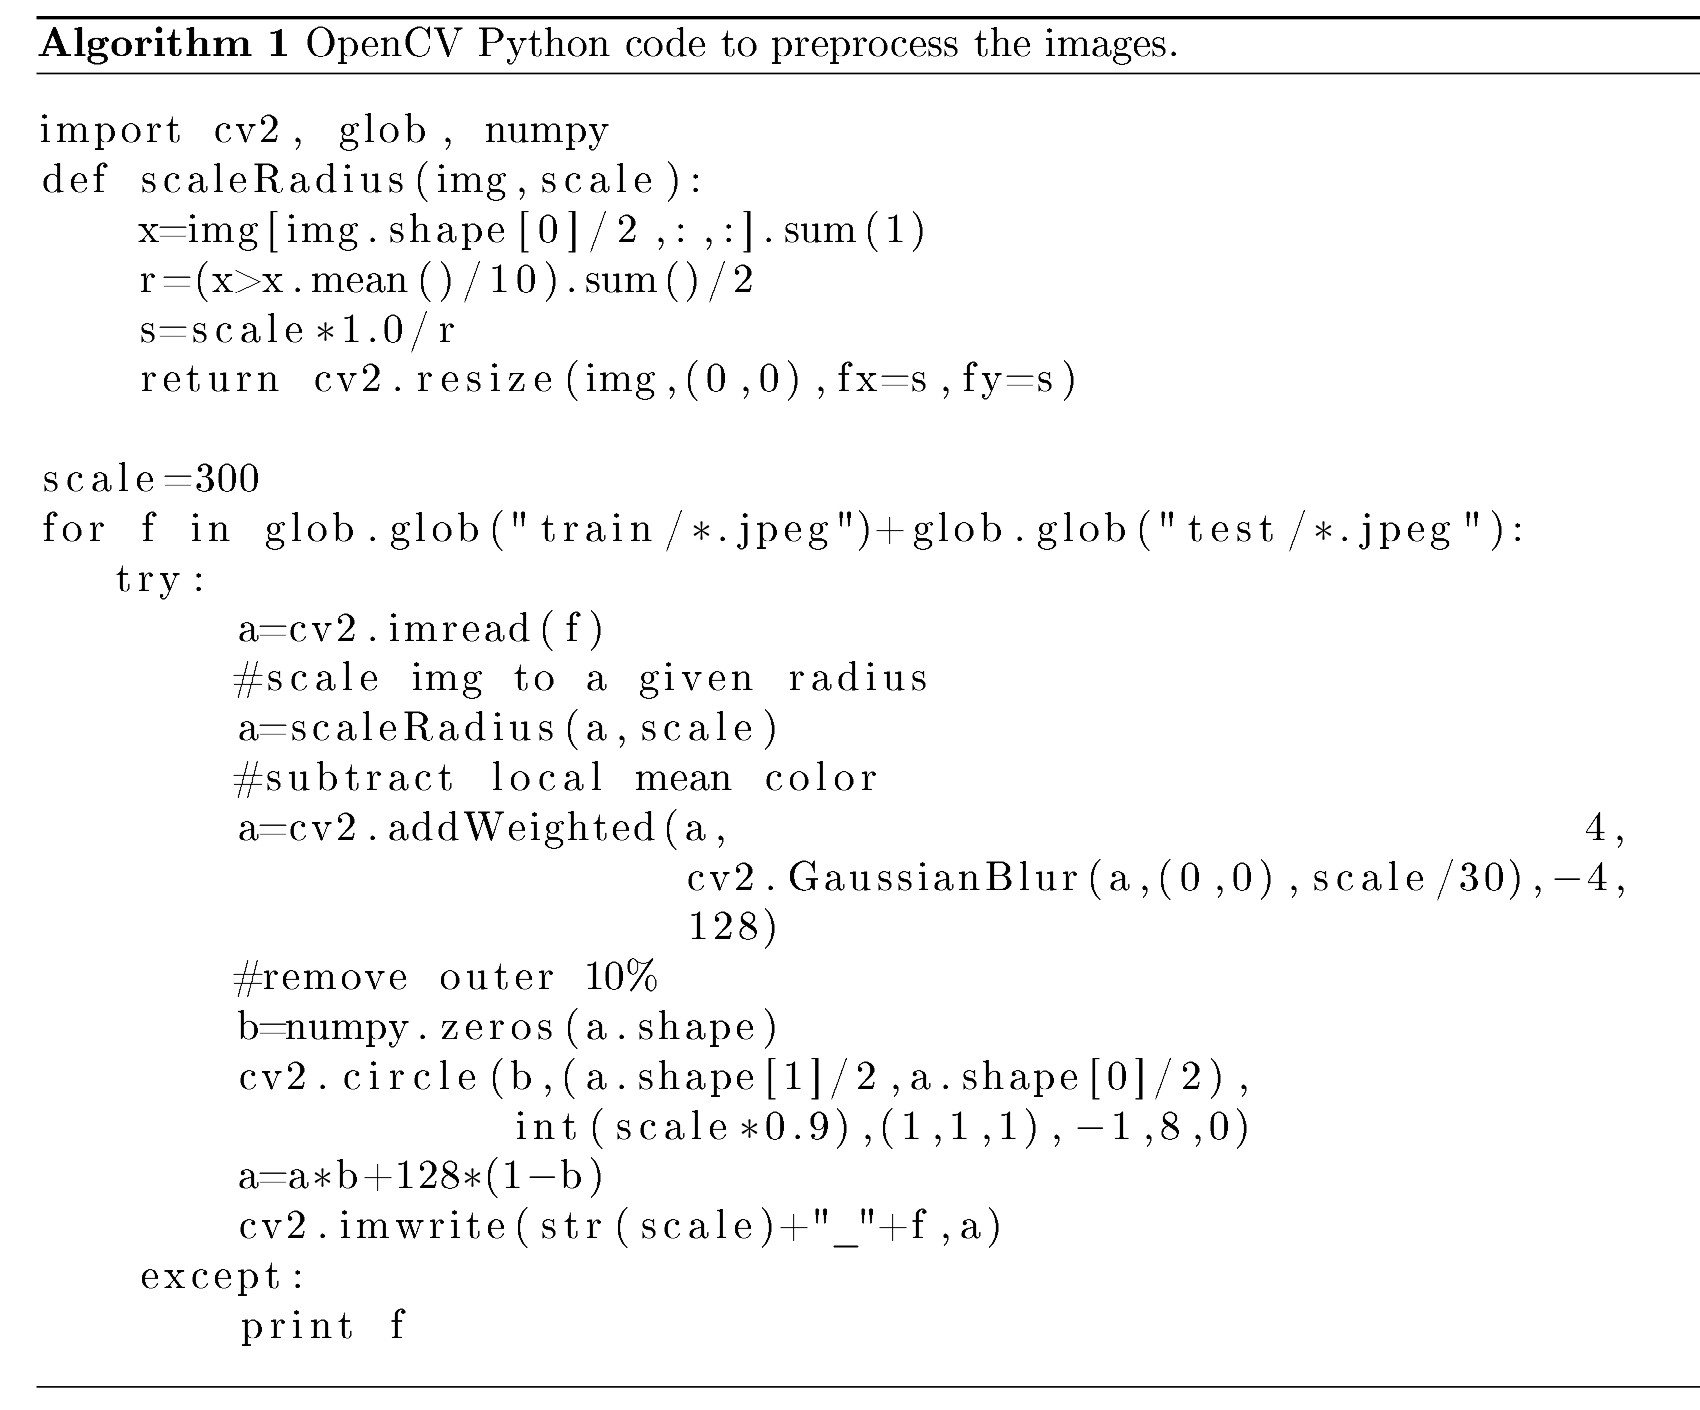
\includegraphics[width=1\textwidth]{imágenes/metodología/algoritmo_braham.jpg}
\caption*{\textit{Fuente: Adaptado de Graham (2015)}}
\end{figure}

Inicialmente las imágenes se redimensionaron para estandarizar el radio del área de 
interés en 300 o 500 píxeles, según el caso. Este paso no solo normaliza la escala entre 
muestras, sino que también optimiza el uso de recursos computacionales en etapas 
posteriores. A continuación se aplicó una normalización del color mediante la sustracción 
del promedio local de intensidad —calculado con un filtro gaussiano— y su remapeo a un 
nivel de gris medio (50\%). Esta corrección mitiga las variaciones de brillo y contraste, 
frecuentes en entornos clínicos reales.

Matemáticamente, la normalización de color se expresa como:

\begin{equation}
I_{norm}(x,y) = \frac{I(x,y) - I_{local\_mean}(x,y)}{\sigma_{local}(x,y) + \epsilon} 
\cdot k + 128
\end{equation}

donde $I(x,y)$ es la intensidad del píxel original, $I_{local\_mean}(x,y)$ es la media 
local calculada con filtro gaussiano, $\sigma_{local}(x,y)$ es la desviación estándar 
local, $\epsilon$ es una constante pequeña para evitar división por cero, y $k$ es un 
factor de escalado.

Por último se enmascaró el 10\% periférico de cada imagen mediante una máscara circular, 
eliminando así artefactos y regiones no informativas mientras se enfoca el análisis en la 
zona central de la retina. De este modo, el algoritmo garantiza que las imágenes 
procesadas presentan una mayor consistencia, lo cual resulta fundamental para etapas 
posteriores de análisis y entrenamiento de modelos. La 
Figura~\ref{fig:preprocesamiento-ejemplo} muestra la implementación paso a paso del 
procedimiento, donde se observa el escalado, la normalización del color y el recorte 
aplicados a cada imagen.

\begin{figure}[H]
	\centering
	\caption{Ejemplo visual del proceso de preprocesamiento aplicado a una imagen de 
fondo de ojo}
	\label{fig:preprocesamiento-ejemplo}
	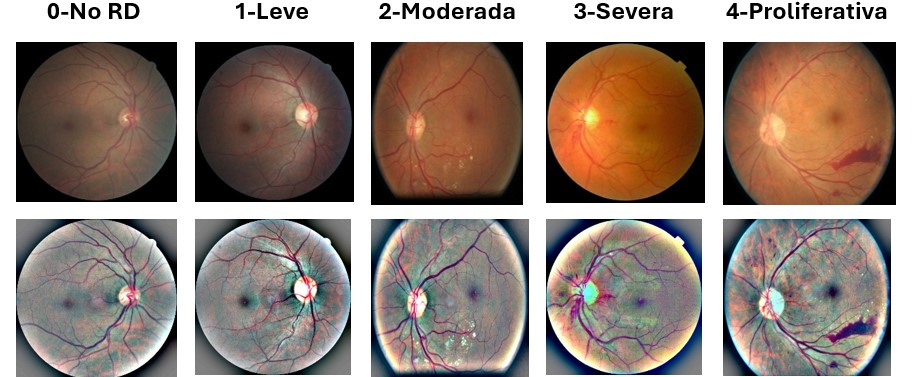
\includegraphics[width=1\textwidth]{imágenes/metodología/preprocesamiento.jpg}
	\caption*{\textit{Fuente: Elaboración propia}}
\end{figure}

\section{TECNOLOGÍAS EMPLEADAS EN EL DESARROLLO}

\subsection{Lenguaje de programación}

En el desarrollo de este trabajo de investigación, se consideraron algunos lenguajes de 
programación para la implementación de las CNNs, cada uno con aspectos particulares en el 
ámbito del procesamiento de imágenes y el aprendizaje profundo. En primer lugar se tomó 
en cuenta R, un lenguaje con una gran variedad de paquetes especializados en modelos 
estadísticos y aprendizaje automático. Sin embargo, su desempeño en tareas de deep 
learning es limitado en comparación con otros lenguajes.

Se consideró también C++, un lenguaje altamente eficiente y optimizado, utilizado en 
aplicaciones donde el rendimiento es crítico. No obstante, su curva de aprendizaje es más 
pronunciada y el desarrollo de modelos de aprendizaje profundo en este lenguaje requiere 
una mayor cantidad de código en comparación con lenguajes de alto nivel.

De este modo, se optó por Python debido a su sintaxis clara y legible que facilita la 
implementación de modelos complejos. Además, cuenta con una amplia comunidad de 
desarrolladores y científicos que contribuyen con documentación, foros de discusión y 
soluciones a problemas frecuentes, lo que resulta en un entorno de desarrollo altamente 
colaborativo. Python cuenta con un ecosistema robusto de herramientas, incluyendo 
librerías como NumPy, Pandas y Matplotlib, que son fundamentales para la manipulación y 
análisis de datos, así como para la visualización de resultados. Asimismo, su 
compatibilidad con aceleradores de hardware, como GPUs y TPUs, permite el entrenamiento 
eficiente de modelos a gran escala, reduciendo significativamente el tiempo de cómputo 
requerido.

\subsection{Entorno de desarrollo integrado (IDE)}

Se evaluaron distintos entornos de desarrollo integrados (IDE), donde cada uno ofrece 
ventajas y características específicas que pueden influir en la ejecución de los modelos. 
Uno de ellos es Jupyter Notebook, una herramienta ampliamente utilizada en investigación 
y desarrollo de proyectos de ciencia de datos debido a su flexibilidad y capacidad para 
ejecutar código de manera interactiva. Sin embargo, su uso requiere una configuración 
manual del entorno y la disponibilidad de recursos computacionales locales.

Google Colab, en cambio, es una opción muy utilizada para el desarrollo en la nube, ya 
que proporciona acceso gratuito a GPUs/TPUs y facilita la colaboración en tiempo real. No 
obstante, presenta ciertas limitaciones en cuanto a la estabilidad de las sesiones; 
acceder a una de sus GPUs gratuitas es difícil debido a la alta demanda, y el entorno se 
desconecta con frecuencia, lo que interrumpe el flujo de trabajo.

En definitiva, se seleccionaron los notebooks en la nube de Kaggle para la implementación 
debido a su estabilidad y a la posibilidad de activar una GPU en cualquier momento, con 
un límite de uso de 30 horas semanales. Esta plataforma proporciona una GPU NVIDIA Tesla 
P100 con 16 GB de memoria, además de la opción de utilizar una NVIDIA T4 x2. Este 
hardware de alto rendimiento optimiza las tareas de aprendizaje automático, agilizando 
tanto el entrenamiento de modelos como la inferencia.

\subsection{Bibliotecas y frameworks}

Se seleccionó TensorFlow junto con su API de alto nivel Keras como framework principal. 
Esta decisión se basó principalmente en que TensorFlow cuenta con una amplia adopción en 
el ámbito clínico y de investigación biomédica, ofreciendo herramientas probadas para el 
procesamiento de imágenes médicas \myfootcite{stanescu2023tensorflow}. Su integración con 
Keras simplifica la implementación de arquitecturas complejas (p. ej., ResNet, 
EfficientNet) mientras mantiene robustez en entornos productivos.

Proporciona un rendimiento eficiente en entornos con GPUs limitadas (como las ofrecidas 
por Kaggle: Tesla P100/T4), gracias a optimizaciones integradas (XLA, Grappler). Keras 
ofrece acceso directo a modelos preentrenados en TensorFlow Hub, ajustables para 
clasificación multiclase de retinopatía. Además, su ecosistema facilita el despliegue en 
clínicas mediante TensorFlow Lite o TF Serving, crucial para una futura implementación en 
entornos hospitalarios.

La suite TensorFlow Extended incluye módulos para aumento de datos (\texttt{tf.image}) y 
preprocesamiento de imágenes médicas (normalización de histogramas, ajuste de contraste), 
esenciales para abordar variabilidad en las imágenes de fondo de ojo (iluminación, 
artefactos). Aunque PyTorch ofrece mayor flexibilidad para investigación experimental, 
requiere más desarrollo manual para estas tareas. TensorFlow/Keras
demostró mayores ventajas en este proyecto al equilibrar productividad, eficiencia 
computacional y facilidad de integración.

\subsection{Especificaciones de hardware}

La Tabla~\ref{tab:hardware-tiempos} resume las especificaciones de hardware utilizadas
para el entrenamiento de los modelos, provistas por el entorno de Kaggle:

\begin{table}[H]
\centering
\renewcommand{\arraystretch}{1.3}
\caption{Especificaciones de hardware}
\label{tab:hardware-tiempos}
\begin{tabularx}{\textwidth}{l X}
\hline
\textbf{Componente} & \textbf{Especificación} \\ \hline
GPU & NVIDIA Tesla P100 (16 GB VRAM) \\
CPU & Intel Xeon (2 cores @ 2.3 GHz) \\
RAM & 13 GB \\
Framework & TensorFlow 2.12.0, Keras 2.12.0 \\
CUDA & 11.8 \\
cuDNN & 8.6 \\ \hline
\end{tabularx}
\caption*{\textit{Fuente: Elaboración propia}}
\end{table}

Los 16 GB de memoria de video (VRAM) de la Tabla~\ref{tab:hardware-tiempos} constituyen
la principal restricción práctica considerada al definir el tamaño de lote (batch size)
utilizado durante el entrenamiento, discutido más adelante en este capítulo.

\section{CONFIGURACIÓN EXPERIMENTAL Y ENTRENAMIENTO} \label{sec:config-experimental}

El proceso de entrenamiento se estructuró en dos fases consecutivas. La primera fase se 
centró en el desarrollo de un modelo para la detección binaria de retinopatía diabética 
(RD), discriminando entre casos positivos (presencia de la enfermedad) y negativos 
(ausencia de la enfermedad). Una vez validado este modelo, se procedió a una segunda fase 
de adaptación para clasificación multiclase, orientada a la categorización de la RD en 
los cinco niveles de gravedad definidos por los estándares clínicos (0: sin RD, 1: leve, 
2: moderada, 3: severa, 4: proliferativa). Esta transición responde a la necesidad de 
alinear el sistema de diagnóstico automático con los protocolos médicos establecidos, 
donde la gradación precisa de la enfermedad es crucial para la toma de decisiones 
terapéuticas.

\subsection{Configuración común para ambos clasificadores}

Para ambos clasificadores se mantuvo un marco experimental común en varios aspectos 
clave. Se implementaron bloques Multi-Head Attention luego de la salida del mapa de 
características de la red previamente entrenada, y capas GaussianNoise entre las capas 
densas. Además, se implementó una estrategia de regularización similar, utilizando en 
ambos casos Dropout, regularización L2 y parada temprana (early stopping).

En cuestión de hiperparámetros se mantuvo el mismo optimizador: Adam con un learning rate 
de $1 \times 10^{-4}$. Se eligió un tamaño de imagen de $224 \times 224$ píxeles, que es 
estándar para muchos modelos preentrenados, lo que permite un equilibrio entre el 
rendimiento computacional y la calidad de la información contenida en las imágenes. Por 
último, para ambos clasificadores se crearon modelos utilizando las mismas redes 
preentrenadas: ResNet50V2, InceptionV3, VGG19 y MobileNetV2.

La configuración de hiperparámetros no fue arbitraria: cada valor responde a alguno de
los siguientes criterios. El \textbf{learning rate} y la \textbf{tasa de Dropout} se
determinaron mediante una búsqueda sistemática (grid search) sobre nueve combinaciones
($1 \times 10^{-3}$, $1 \times 10^{-4}$ y $1 \times 10^{-5}$ para el learning rate;
$0.2$, $0.3$ y $0.5$ para el Dropout), entrenando y evaluando cada combinación sobre el
conjunto de validación; la combinación con mejor F1-score
($1 \times 10^{-4}$ y $0.2$, respectivamente) fue la seleccionada. La
\textbf{regularización L2} se probó experimentalmente sobre la mejor combinación
encontrada: su efecto sobre el F1-score y el AUC-ROC resultó marginal, pero se mantuvo
como regularizador adicional junto con Dropout y GaussianNoise. El \textbf{tamaño de
lote} (batch size) de 16 responde a una restricción computacional práctica, dado el uso
de GPUs Tesla P100/T4 provistas por Kaggle (Sección~\ref{sec:preprocesamiento}) en
conjunto con la arquitectura MobileNetV2 y el bloque de atención, que incrementan el
consumo de memoria por lote. La \textbf{paciencia de early stopping} (5 épocas) y la
\textbf{desviación estándar de GaussianNoise} (0.2) corresponden a valores de uso común
en la literatura de regularización de redes neuronales profundas, dentro de los rangos
habitualmente reportados para evitar tanto un entrenamiento prematuramente interrumpido
como una perturbación excesiva de las activaciones. El \textbf{número de cabezas de
atención} (4) sigue la práctica común en bloques de atención de tamaño moderado
acoplados a arquitecturas CNN, donde se busca capturar múltiples subespacios de
representación sin incrementar excesivamente el número de parámetros del modelo.

La Tabla~\ref{tab:hiperparametros} resume los hiperparámetros específicos utilizados en
cada tipo de clasificador:

\begin{table}[H]
\centering
\renewcommand{\arraystretch}{1.3}
\caption{Configuración de hiperparámetros para clasificadores binario y multiclase}
\label{tab:hiperparametros}
\begin{tabularx}{\textwidth}{l X >{\centering\arraybackslash}p{3.2cm} >{\centering\arraybackslash}p{3.2cm}}
\hline
\textbf{Hiperparámetro} & \textbf{Descripción} & \textbf{Binario} & \textbf{Multiclase}
\\ \hline
Tamaño de entrada & Dimensiones de imagen & $224 \times 224$ & $224 \times 224$ \\
Optimizador & Algoritmo de optimización & Adam & Adam \\
Learning rate & Tasa de aprendizaje & $1 \times 10^{-4}$ & $1 \times 10^{-4}$ \\
Batch size & Tamaño de lote & 16 & 16 \\
Épocas máximas & Número máximo de épocas & 50 & 50 \\
Dropout rate & Tasa de abandono & 0.2 & 0.2 \\
L2 regularization & Factor de regularización & 0.01 & 0.01 \\
GaussianNoise std & Desviación estándar del ruido & 0.2 & 0.2 \\
Early stopping patience & Paciencia para parada temprana & 5 épocas & 5 épocas \\
Función de pérdida & Función objetivo & Binary crossentropy & Sparse categorical crossentropy \\
Cabezas de atención & Número de cabezas en Multi-Head Attention & 4 & 4 \\
Capas densas & Configuración del top model & 512-256 & 256-128 \\
Activación salida & Función de activación final & Sigmoid & Softmax \\
Neuronas salida & Número de clases & 1 & 5 \\ \hline
\end{tabularx}
\caption*{\textit{Fuente: Elaboración propia}}
\end{table}

\subsection{Configuración experimental para el clasificador binario}

Para el clasificador binario, se utilizaron capas densas con 512 y 256 neuronas, 
intercaladas entre ellas. Esta configuración de top model es ampliamente utilizada en 
problemas de clasificación binaria con redes preentrenadas. Las funciones de activación 
utilizadas en estas capas fueron ReLU, mientras que la capa de salida fue una capa densa 
con una sola neurona y función de activación Sigmoid, apropiada para clasificación 
binaria.

Todas las capas convolucionales de cada red base fueron congeladas durante la fase de 
entrenamiento, permitiendo entrenar únicamente las capas densas superiores y los bloques 
de atención. Esto facilitó evaluar la capacidad de transferencia de características desde 
el dominio general de ImageNet al dominio específico de imágenes médicas, con un 
entrenamiento rápido y controlado.

\subsection{Configuración experimental para el clasificador multiclase}

Para el clasificador multiclase, se utilizaron capas densas con 256 y 128 neuronas 
intercaladas entre ellas. Este tipo de configuración de top model suele ser de los más 
utilizados en problemas similares \myfootcite{mutawa2023transfer}. Las funciones de 
activación utilizadas en estas capas fueron ReLU. La capa de salida fue una densa con 
cinco neuronas, una para cada nivel de RD, y función de activación Softmax.

Esta combinación de funciones de activación ha tenido bastante éxito, pues han demostrado 
un alto rendimiento y eficiencia. En muchos trabajos recopilatorios se puede ver que esta 
combinación de funciones de activación —ReLU para capas intermedias y Softmax para capa 
de salida— suele ser la más común y la que mejores resultados arroja 
\myfootcite{nadeem2022deep}. En una investigación de 2020 realizada por Asadi y Jiang 
\myfootcite{asadi2020approximation}, se demostró que ambas funciones de activación son 
aproximadores universales, dándole un fundamento teórico más robusto a su uso práctico.

Todas las capas convolucionales de cada red base fueron congeladas durante esta fase de 
experimentación, permitiendo entrenar únicamente las capas densas superiores. Se utilizó 
el optimizador Adam y la función de pérdida sparse categorical crossentropy, adecuada 
para clasificación multiclase con etiquetas en formato entero. El uso de esta función de 
pérdida ha demostrado ser más efectivo en tareas similares 
\myfootcite{palaniappan2023wide}.

Al concluir el entrenamiento, los modelos fueron evaluados tanto en el conjunto de 
entrenamiento como en el de validación. Se generaron métricas clave: recuperación 
(recall), puntuación F1 y exactitud (accuracy) mediante el informe de clasificación de 
scikit-learn. Los resultados se almacenaron y organizaron para su análisis comparativo. 
Además, se elaboraron gráficos que muestran la evolución de la pérdida y exactitud 
durante el entrenamiento, lo que permitió observar visualmente el rendimiento diferencial 
de cada arquitectura.

\subsection{Arquitectura completa del modelo}

La Figura~\ref{fig:arquitectura-modelo} muestra la arquitectura completa implementada, 
desde la entrada de la imagen hasta la capa de salida:

\begin{figure}[H]
\centering
\caption{Arquitectura completa del modelo propuesto con bloques de atención y 
regularización}
\label{fig:arquitectura-modelo}
\begin{center}
\shorthandoff{>}
\begin{tikzpicture}[node distance=1cm]
\node[draw, rectangle] (input) {Imagen de entrada $224 \times 224 \times 3$};
\node[draw, rectangle, below=of input] (base) {Base CNN preentrenada (congelada)};
\node[draw, rectangle, below=of base] (attention) {Multi-Head Attention (4 heads)};
\node[draw, rectangle, below=of attention] (gap) {Global Average Pooling};
\node[draw, rectangle, below=of gap] (noise1) {GaussianNoise ($\sigma=0.2$)};
\node[draw, rectangle, below=of noise1] (dense1) {Dense (512/256) + ReLU + Dropout (0.2)
+ L2};
\node[draw, rectangle, below=of dense1] (noise2) {GaussianNoise ($\sigma=0.2$)};
\node[draw, rectangle, below=of noise2] (dense2) {Dense (256/128) + ReLU + Dropout (0.2)
+ L2};
\node[draw, rectangle, below=of dense2] (output) {Dense (1/5) + Sigmoid/Softmax};

\draw[->] (input) -- (base);
\draw[->] (base) -- (attention);
\draw[->] (attention) -- (gap);
\draw[->] (gap) -- (noise1);
\draw[->] (noise1) -- (dense1);
\draw[->] (dense1) -- (noise2);
\draw[->] (noise2) -- (dense2);
\draw[->] (dense2) -- (output);
\end{tikzpicture}
\shorthandon{>}
\end{center}
\caption*{\textit{Fuente: Elaboración propia}}
\end{figure}

En la Figura~\ref{fig:arquitectura-modelo} puede observarse que el flujo de información
pasa primero por la base CNN preentrenada (congelada) y el bloque de atención, seguido de
dos capas densas intercaladas con GaussianNoise y regularización (Dropout y L2), hasta
llegar a la capa de salida, cuyo número de neuronas y función de activación (Sigmoid o
Softmax) dependen de si se trata del clasificador binario o multiclase, respectivamente.

\subsection{Reproducibilidad y disponibilidad de código}

Para garantizar la reproducibilidad de los experimentos, se fijaron las siguientes 
semillas aleatorias:

\begin{itemize}
    \item Semilla Python random: 42
    \item Semilla NumPy: 42
    \item Semilla TensorFlow: 42
\end{itemize}

Las versiones específicas de las bibliotecas utilizadas fueron:
\begin{itemize}
    \item Python: 3.10.12
    \item TensorFlow: 2.12.0
    \item Keras: 2.12.0
    \item NumPy: 1.23.5
    \item Pandas: 1.5.3
    \item OpenCV: 4.7.0
    \item scikit-learn: 1.2.2
\end{itemize}

El código fuente completo de los experimentos está disponible en el repositorio de Kaggle 
asociado al proyecto, permitiendo la replicación exacta de todos los procedimientos 
descritos.

\section{MÉTRICAS DE EVALUACIÓN} \label{sec:metricas-evaluacion}

En los estudios de clasificación médica existen diferentes métricas de desempeño
ampliamente utilizadas. La exactitud, la sensibilidad, la especificidad, la precisión y
el F1-score son algunas de ellas, y estas medidas se emplean para evaluar el rendimiento
de un método utilizado. En las fórmulas de la Tabla~\ref{tab:metricas-evaluacion}, TP
(True Positives) y FP (False Positives) representan el número de diagnósticos
verdaderos positivos y falsos positivos, respectivamente; TN (True Negatives) y FN
(False Negatives) representan el número de diagnósticos verdaderos negativos y falsos
negativos; y N es el número total de muestras.

\begin{table}[H]
\centering
\renewcommand{\arraystretch}{1.8}
\small
\caption{Métricas de evaluación utilizadas}
\label{tab:metricas-evaluacion}
\begin{tabularx}{\textwidth}{@{}l X c@{}}
\hline
\textbf{Métrica} & \textbf{Descripción} & \textbf{Fórmula} \\ \hline
Exactitud (Accuracy) & Proporción de predicciones correctas sobre el total de
muestras; poco informativa si las clases están desbalanceadas. &
$\frac{TP + TN}{N}$ \\
Sensibilidad (Recall) & Proporción de casos positivos (con RD) detectados
correctamente; crucial para minimizar casos no detectados. &
$\frac{TP}{TP + FN}$ \\
Especificidad & Proporción de casos negativos (sin RD) identificados correctamente;
reduce las derivaciones innecesarias. &
$\frac{TN}{TN + FP}$ \\
Precisión (Precision) & Proporción de predicciones positivas que realmente lo son;
evita el sobrediagnóstico. &
$\frac{TP}{TP + FP}$ \\
F1-score & Media armónica entre precisión y sensibilidad; balancea falsos positivos
y falsos negativos. &
$2 \cdot \frac{P \cdot S}{P + S}$ \\ \hline
\end{tabularx}
\caption*{\textit{Fuente: Elaboración propia}}
\end{table}

Adicionalmente, se calculó el área bajo la curva ROC (AUC-ROC), que proporciona una
medida robusta del desempeño del clasificador independiente del umbral de decisión. Un
valor de AUC cercano a 1.0 indica un excelente desempeño discriminatorio.

Aunque todas las métricas anteriores aportan información complementaria, no todas tienen
la misma relevancia para el problema clínico abordado en este trabajo. Dado que el
sistema se plantea principalmente como una herramienta de \textbf{tamizaje} —es decir,
un primer filtro que decide qué pacientes requieren remisión a evaluación oftalmológica
especializada—, la \textbf{sensibilidad se considera la métrica prioritaria}. Un falso
negativo en este contexto implica que un paciente con retinopatía diabética no sea
remitido para evaluación especializada, retrasando un diagnóstico y tratamiento
oportunos; en cambio, un falso positivo implica, en el peor de los casos, una remisión
innecesaria a un especialista, un costo considerablemente menor en términos clínicos.
Esta priorización de la sensibilidad es, además, el criterio que sustenta la elección del
umbral de decisión: en la Sección~\ref{subsec:umbral-decision} el umbral se optimiza
maximizando el F1-score (que pondera sensibilidad y precisión por igual) en lugar de
utilizar el valor por defecto de 0.5, precisamente para evitar que el modelo favorezca la
precisión a costa de dejar pasar casos reales de RD.

Para evaluar la robustez estadística de las métricas obtenidas, se aplicó la técnica de
bootstrap con 1,000 iteraciones de remuestreo, calculando intervalos de confianza del
95\% para cada métrica. Esto permite estimar la variabilidad de las medidas de desempeño
y proporciona una evaluación más rigurosa de la confiabilidad del modelo.

En este estudio, todos los parámetros de evaluación mencionados se utilizaron para
caracterizar el desempeño del sistema propuesto desde distintas perspectivas
complementarias, aunque, como se indicó, la sensibilidad se prioriza como criterio
principal de decisión dado el enfoque de tamizaje del sistema, tanto en clasificación
binaria como multiclase.
  % Modelo CNN 
\chapter{RESULTADOS EXPERIMENTALES} \label{chap:resultados}

Este capítulo presenta los resultados obtenidos de la implementación y evaluación de los 
modelos de clasificación de retinopatía diabética desarrollados, se organiza en dos secciones principales: 
primero se presentan los resultados de la clasificación binaria (presencia/ausencia de 
RD), incluyendo la comparación de arquitecturas CNN, el impacto del preprocesamiento 
mediante filtrado, la optimización del umbral de decisión, el análisis estadístico 
mediante bootstrap y la validación externa en tres datasets independientes. 
Posteriormente se exponen los resultados de la clasificación multiclase (gradación en 
cinco niveles de severidad), con énfasis en el análisis comparativo del desempeño al 
procesar diferentes canales de color (RGB, rojo, verde, azul).

\section{CLASIFICACIÓN BINARIA}

\subsection{Comparación de arquitecturas CNN preentrenadas}

Se implementó una estrategia de aprendizaje por transferencia utilizando diversas redes 
preentrenadas disponibles en Keras Applications. Debido a que cada red requiere un tamaño 
de entrada específico, se seleccionaron finalmente VGG19, ResNet50V2, InceptionV3 y 
MobileNetV2, todas con tamaños de entrada compatibles ($224 \times 224$ píxeles). Estas 
arquitecturas permiten analizar la estrategia tanto desde el punto de vista de desempeño 
como de eficiencia computacional, considerando la velocidad de inferencia y la cantidad 
de parámetros. Además, se eligieron para comparar el comportamiento de redes clásicas, 
como VGG19, frente a arquitecturas más modernas, como MobileNetV2.

En la Tabla~\ref{tab:comparacion_redes} se presentan los resultados obtenidos al entrenar
el modelo CNN variando entre estas redes preentrenadas, fijando un umbral de decisión de
0.5, con el objetivo de identificar la red base con mejor desempeño en la clasificación
binaria en términos de precisión, sensibilidad, F1-score y especificidad. Dado que RD se
define como la clase positiva y No RD como la clase negativa, la sensibilidad (recall de
RD) y la especificidad (recall de No RD) ya tienen una interpretación única respecto a
esa definición; por ello, a diferencia de un reporte de métricas por clase, se presenta
una sola fila por arquitectura en lugar de repetir ambas métricas para cada clase.

\begin{table}[ht!]
	\centering
	\renewcommand{\arraystretch}{1.2}
	\caption{Desempeño de redes preentrenadas para clasificación binaria de
retinopatía diabética usando el dataset original de Kaggle (RD como clase positiva)}
	\label{tab:comparacion_redes}
	\begin{tabularx}{\textwidth}{l Y Y Y Y}
		\toprule
		Red Preentrenada & Sensibilidad & Especificidad & Precisión & F1-score \\
		\midrule
		MobileNetV2 & \textbf{0.95} & \textbf{0.94} & \textbf{0.95} & \textbf{0.95} \\
		ResNet50V2 & 0.77 & 0.78 & 0.77 & 0.77 \\
		InceptionV3 & 0.71 & 0.72 & 0.71 & 0.71 \\
		VGG19 & 0.86 & 0.85 & 0.86 & 0.86 \\
		\bottomrule
	\end{tabularx}
	\caption*{\textit{Fuente: Elaboración propia}}
\end{table}

Según la Tabla~\ref{tab:comparacion_redes}, MobileNetV2 fue la arquitectura con mejor
desempeño global: alcanzó la mayor exactitud
(0.95) y F1-score (0.95), combinando además un tiempo de inferencia relativamente bajo en
comparación con las demás redes. VGG19 presentó métricas intermedias (F1 $\approx$ 0.86) 
pero con un tiempo de inferencia mayor, mientras que ResNet50V2 e InceptionV3 mostraron 
rendimientos inferiores (F1 $\approx$ 0.77 y 0.71, respectivamente), con tiempos de 
inferencia moderados.

Esta superioridad de MobileNetV2 puede atribuirse a su arquitectura eficiente basada en 
bloques residuales invertidos y cuellos de botella lineales, que proporciona una 
regularización implícita beneficiosa cuando el conjunto de datos disponible es limitado. 
En contraste, VGG19, a pesar de su profundidad, exhibió tendencia al sobreajuste debido a 
su elevado número de parámetros en capas completamente conectadas y ausencia de 
conexiones residuales.

En conclusión, MobileNetV2 fue seleccionada como \textbf{backbone} para los experimentos
adicionales, al equilibrar precisión, sensibilidad y eficiencia computacional, lo
que la hace más adecuada para un escenario de tamizaje clínico donde la velocidad de
procesamiento es relevante. La Figura~\ref{fig:conf-matrix-original} presenta las
matrices de confusión de las cuatro redes, donde se observa que MobileNetV2 concentra la
mayor proporción de aciertos en la diagonal principal (99 y 100 sobre 105 casos por
clase) y el menor número de falsos negativos (5), mientras que ResNet50V2 e InceptionV3
muestran una dispersión de errores considerablemente mayor entre ambas clases.

\begin{figure}[ht!]
	\centering
	\renewcommand{\arraystretch}{1.2}
	\caption{Matrices de confusión para las diferentes redes preentrenadas en
clasificación binaria}
	\label{fig:conf-matrix-original}

	% Matriz 1 - VGG19
	\begin{minipage}{0.45\textwidth}
		\centering
		\begin{tabular}{c c c}
			& \multicolumn{2}{c}{\textbf{Predicción}} \\
			& \textbf{No RD} & \textbf{RD} \\ \hline
			\multirow{2}{*}{\textbf{Real}}
			No RD & 90 & 15 \\
			\multicolumn{1}{r}{RD} & 15 & 90 \\
		\end{tabular}
		\caption*{(a) VGG19}
	\end{minipage}
	\hfill
	% Matriz 2 - MobileNetV2
	\begin{minipage}{0.45\textwidth}
		\centering
		\begin{tabular}{c c c}
			& \multicolumn{2}{c}{\textbf{Predicción}} \\
			& \textbf{No RD} & \textbf{RD} \\ \hline
			\multirow{2}{*}{\textbf{Real}}
			No RD & 99 & 6 \\
			\multicolumn{1}{r}{RD} & 5 & 100 \\
		\end{tabular}
		\caption*{(b) MobileNetV2}
	\end{minipage}

	\vspace{0.5cm}

	% Matriz 3 - ResNet50V2
	\begin{minipage}{0.45\textwidth}
		\centering
		\begin{tabular}{c c c}
			& \multicolumn{2}{c}{\textbf{Predicción}} \\
			& \textbf{No RD} & \textbf{RD} \\ \hline
			\multirow{2}{*}{\textbf{Real}}
			No RD & 82 & 23 \\
			\multicolumn{1}{r}{RD} & 28 & 77 \\
		\end{tabular}
		\caption*{(c) ResNet50V2}
	\end{minipage}
	\hfill
	% Matriz 4 - InceptionV3
	\begin{minipage}{0.45\textwidth}
		\centering
		\begin{tabular}{c c c}
			& \multicolumn{2}{c}{\textbf{Predicción}} \\
			& \textbf{No RD} & \textbf{RD} \\ \hline
			\multirow{2}{*}{\textbf{Real}}
			No RD & 80 & 25 \\
			\multicolumn{1}{r}{RD} & 30 & 75 \\
		\end{tabular}
		\caption*{(d) InceptionV3}
	\end{minipage}
	\caption*{\textit{Fuente: Elaboración propia}}
\end{figure}

En el contexto clínico de este trabajo, los dos tipos de error de la Figura~\ref{fig:conf-matrix-original}
no son equivalentes: un \textbf{falso negativo} (un paciente con RD clasificado como
sano) implica que dicho paciente no sea remitido a evaluación oftalmológica
especializada, retrasando su diagnóstico y tratamiento; un \textbf{falso positivo} (un
paciente sano clasificado como RD) implica, en cambio, una remisión innecesaria, un costo
clínico considerablemente menor. Analizando las cuatro redes bajo este criterio,
MobileNetV2 presenta el mejor balance (5 falsos negativos y 6 falsos positivos sobre 105
casos por clase), mientras que VGG19 muestra un número similar de ambos tipos de error
(15 y 15). ResNet50V2 e InceptionV3, en cambio, no solo presentan más errores en total,
sino que estos se concentran de forma más pronunciada en falsos negativos que en falsos
positivos (28 frente a 23 en ResNet50V2, y 30 frente a 25 en InceptionV3):
proporcionalmente, estas dos redes dejan sin detectar más casos reales de RD de los que
remiten innecesariamente, lo que constituye el patrón de error clínicamente menos
deseable para una herramienta de tamizaje y refuerza, junto con las métricas agregadas de
la Tabla~\ref{tab:comparacion_redes}, la decisión de descartar ambas arquitecturas para
los experimentos posteriores.

\subsection{Impacto del preprocesamiento mediante filtrado}

Con el objetivo de mejorar la calidad visual y resaltar características relevantes, se 
aplicó un filtrado previo a las imágenes del fondo de ojo utilizando las mismas redes 
preentrenadas. El algoritmo de preprocesamiento de Ben Graham, descrito en el 
Capítulo~\ref{chap:metodologia}, consistió en normalización de color mediante sustracción 
del promedio local con filtro gaussiano y enmascaramiento del 10\% periférico de la 
imagen.

Tras evaluar los modelos se observó una mejora en el rendimiento: el tiempo de inferencia
se redujo respecto al experimento sin filtrado, y se alcanzaron métricas más altas de
desempeño, con F1-score de 0.96 para MobileNetV2, reflejando su superioridad. La
Tabla~\ref{tab:impacto-filtrado} compara sensibilidad, especificidad, precisión y
F1-score de las cuatro arquitecturas antes y después de aplicar el filtrado, mostrando
una mejora consistente en las cuatro métricas para todas las redes.

\begin{table}[ht!]
	\centering
	\renewcommand{\arraystretch}{1.2}
	\caption{Comparación del rendimiento de las redes preentrenadas sin y con 
filtrado de imágenes}
	\label{tab:impacto-filtrado}
	\begin{tabularx}{\textwidth}{Y Y Y Y Y Y}
		\toprule
		Red Preentrenada & Sensibilidad & Especificidad & Precisión & F1-score & 
Dataset \\
		\midrule
		\multirow{2}{*}{MobileNetV2} & 0.95 & \textbf{0.95} & 0.95 & 0.95 & Original \\
		& \textbf{0.96} & \textbf{0.95} & \textbf{0.96} & \textbf{0.96} & Filtrado \\
		\midrule
		\multirow{2}{*}{ResNet50V2} & 0.77 & 0.78 & 0.77 & 0.77 & Original \\
		& 0.81 & 0.82 & 0.81 & 0.81 & Filtrado \\
		\midrule
		\multirow{2}{*}{InceptionV3} & 0.71 & 0.72 & 0.71 & 0.71 & Original \\
		& 0.74 & 0.75 & 0.74 & 0.74 & Filtrado \\
		\midrule
		\multirow{2}{*}{VGG19} & 0.86 & 0.85 & 0.86 & 0.86 & Original \\
		& 0.89 & 0.88 & 0.89 & 0.89 & Filtrado \\
		\bottomrule
	\end{tabularx}
	\caption*{\textit{Fuente: Elaboración propia}}
\end{table}

Como muestra la Tabla~\ref{tab:impacto-filtrado}, la aplicación de filtrado incrementó
consistentemente el rendimiento de todas las redes, manteniendo la jerarquía de
desempeño: VGG19 mostró un F1-score intermedio
($\approx$0.89), mientras que ResNet50V2 e InceptionV3 tuvieron incrementos moderados 
($\approx$0.81 y 0.74, respectivamente). El cambio más notable fue la reducción de falsos 
positivos en MobileNetV2 (aproximadamente 4 vs. 6 sin filtrado), lo que mejora la 
especificidad clínica y disminuye derivaciones innecesarias. Los falsos negativos
también se redujeron ligeramente (3 vs. 5), lo cual es clínicamente relevante: implica
menos casos reales de RD sin detectar, el tipo de error más costoso en un escenario de
tamizaje.

Este resultado confirma la importancia del preprocesamiento robusto para mitigar
variaciones de brillo y contraste inherentes a la captura de imágenes en entornos
clínicos heterogéneos, donde las condiciones de iluminación y los equipos de adquisición
varían considerablemente. La Figura~\ref{fig:conf-matrix-filtrado} muestra las matrices
de confusión resultantes tras aplicar el filtrado: para MobileNetV2 se aprecia la
reducción de falsos positivos señalada anteriormente (de 6 a 4 casos), mientras que en
VGG19, ResNet50V2 e InceptionV3 la diagonal principal se refuerza de manera consistente
respecto a las matrices sin filtrado de la Figura~\ref{fig:conf-matrix-original}. El
filtrado también mejora, aunque de forma más modesta, el desbalance entre falsos
negativos y falsos positivos observado antes en ResNet50V2 e InceptionV3: los falsos
negativos de ResNet50V2 bajan de 28 a 22 (por debajo de sus 23 falsos positivos), y los
de InceptionV3 bajan de 30 a 26, acercándose a sus 25 falsos positivos. Es decir, además
de mejorar el desempeño agregado, el preprocesamiento reduce específicamente el tipo de
error más costoso desde la perspectiva del tamizaje clínico.

\begin{figure}[ht!]
	\centering
	\renewcommand{\arraystretch}{1.2}
	\caption{Matrices de confusión para las redes preentrenadas utilizando imágenes
con filtrado}
	\label{fig:conf-matrix-filtrado}

	% Matriz 1 - VGG19
	\begin{minipage}{0.45\textwidth}
		\centering
		\begin{tabular}{c c c}
			& \multicolumn{2}{c}{\textbf{Predicción}} \\
			& \textbf{No RD} & \textbf{RD} \\ \hline
			\multirow{2}{*}{\textbf{Real}}
			No RD & 88 & 12 \\
			\multicolumn{1}{r}{RD} & 10 & 89 \\
		\end{tabular}
		\caption*{(a) VGG19 con filtrado}
	\end{minipage}
	\hfill
	% Matriz 2 - MobileNetV2
	\begin{minipage}{0.45\textwidth}
		\centering
		\begin{tabular}{c c c}
			& \multicolumn{2}{c}{\textbf{Predicción}} \\
			& \textbf{No RD} & \textbf{RD} \\ \hline
			\multirow{2}{*}{\textbf{Real}}
			No RD & 96 & 4 \\
			\multicolumn{1}{r}{RD} & 3 & 96 \\
		\end{tabular}
		\caption*{(b) MobileNetV2 con filtrado}
	\end{minipage}

	\vspace{0.5cm}

	% Matriz 3 - ResNet50V2
	\begin{minipage}{0.45\textwidth}
		\centering
		\begin{tabular}{c c c}
			& \multicolumn{2}{c}{\textbf{Predicción}} \\
			& \textbf{No RD} & \textbf{RD} \\ \hline
			\multirow{2}{*}{\textbf{Real}}
			No RD & 82 & 23 \\
			\multicolumn{1}{r}{RD} & 22 & 81 \\
		\end{tabular}
		\caption*{(c) ResNet50V2 con filtrado}
	\end{minipage}
	\hfill
	% Matriz 4 - InceptionV3
	\begin{minipage}{0.45\textwidth}
		\centering
		\begin{tabular}{c c c}
			& \multicolumn{2}{c}{\textbf{Predicción}} \\
			& \textbf{No RD} & \textbf{RD} \\ \hline
			\multirow{2}{*}{\textbf{Real}}
			No RD & 75 & 25 \\
			\multicolumn{1}{r}{RD} & 26 & 74 \\
		\end{tabular}
		\caption*{(d) InceptionV3 con filtrado}
	\end{minipage}
	\caption*{\textit{Fuente: Elaboración propia}}
\end{figure}

\subsection{Optimización del umbral de decisión} \label{subsec:umbral-decision}

El umbral de decisión de los modelos fue optimizado mediante la maximización del F1-score 
en el conjunto de validación. Como se observa en la Tabla~\ref{tab:umbral-optimo}, 
MobileNetV2 alcanzó un umbral óptimo de 0.4826, mientras que las demás redes presentan 
valores ligeramente diferentes.

\begin{table}[ht!]
	\centering
	\renewcommand{\arraystretch}{1.2}
	\caption{Umbral de decisión óptimo obtenido para cada red preentrenada en 
clasificación binaria}
	\label{tab:umbral-optimo}
	\begin{tabular}{lc}
		\hline
		Modelo & Umbral Óptimo \\ \hline
		VGG19 & 0.4903 \\
		ResNet50V2 & 0.4607 \\
		InceptionV3 & 0.4532 \\
		MobileNetV2 & 0.4826 \\
		\hline
	\end{tabular}
	\caption*{\textit{Fuente: Elaboración propia}}
\end{table}

Este procedimiento identificó, para MobileNetV2 (Tabla~\ref{tab:umbral-optimo}), un
umbral óptimo de 0.4826, que resultó en un F1-score de
0.9519 con filtrado. El modelo muestra un balance adecuado entre la
detección de casos positivos y la reducción de falsos positivos, lo que lo hace apropiado 
para tareas de tamizaje. Con este umbral, por cada 1,000 pacientes examinados se 
esperarían aproximadamente: 476 verdaderos positivos y 451 verdaderos negativos, 50 
falsos negativos (casos no detectados de RD) y 24 falsos positivos (pacientes sin RD que 
serían derivados innecesariamente).

La optimización del umbral representa una mejora sutil pero relevante en el contexto
clínico, ya que permite ajustar el balance entre sensibilidad y especificidad según las
prioridades del programa de tamizaje. Un umbral menor a 0.5 favorece la sensibilidad, lo
cual es apropiado para detección temprana donde se prioriza minimizar casos no detectados.
La Tabla~\ref{tab:comparacion-umbral} contrasta, para cada arquitectura, las métricas
obtenidas con el umbral fijo de 0.5 frente a las obtenidas con su umbral óptimo
respectivo: MobileNetV2 y VGG19 muestran una mejora en el F1-score, mientras que en
ResNet50V2 e InceptionV3 el F1-score se mantiene igual; en las cuatro arquitecturas el
recall aumenta respecto al umbral fijo, en la mayoría de los casos a costa de una
precisión ligeramente menor.

\begin{table}[ht!]
	\centering
	\renewcommand{\arraystretch}{1.2}
	\caption{Comparación del rendimiento de las redes preentrenadas en clasificación
binaria utilizando el umbral fijo (0.5) y el umbral óptimo calculado}
	\label{tab:comparacion-umbral}
	\begin{tabularx}{\textwidth}{Y Y Y Y Y Y}
		\toprule
		Modelo & Umbral & Exactitud & Precisión & Recall & F1-score \\
		\midrule
		\multirow{2}{*}{VGG19} & 0.5 & 0.88 & 0.87 & 0.86 & 0.86 \\
		& Óptimo & 0.87 & 0.86 & 0.89 & 0.87 \\
		\midrule
		\multirow{2}{*}{ResNet50V2} & 0.5 & 0.81 & 0.81 & 0.81 & 0.81 \\
		& Óptimo & 0.80 & 0.80 & 0.83 & 0.81 \\
		\midrule
		\multirow{2}{*}{InceptionV3} & 0.5 & 0.74 & 0.74 & 0.74 & 0.74 \\
		& Óptimo & 0.73 & 0.73 & 0.76 & 0.74 \\
		\midrule
		\multirow{2}{*}{MobileNetV2} & 0.5 & 0.95 & 0.95 & 0.95 & 0.95 \\
		& Óptimo & 0.96 & 0.96 & 0.96 & 0.96 \\
		\bottomrule
	\end{tabularx}
	\caption*{\textit{Fuente: Elaboración propia}}
\end{table}

\subsection{Análisis estadístico mediante bootstrap}

Es importante precisar que todos los resultados reportados en este capítulo —incluyendo
los de la Tabla~\ref{tab:comparacion_redes} y las secciones posteriores— corresponden a
un único entrenamiento sobre una única partición de los datos (con semilla aleatoria
fija), y no al promedio de varias ejecuciones ni a un esquema de validación cruzada
($k$-fold). Esta decisión responde a las restricciones computacionales del proyecto,
descritas en la Sección~\ref{sec:config-experimental}: entrenar y evaluar cuatro
arquitecturas preentrenadas, en dos escenarios de clasificación (binario y multiclase),
bajo múltiples configuraciones de preprocesamiento y canales de color, ya representa un
número considerable de entrenamientos; repetir cada uno de ellos varias veces o mediante
validación cruzada habría multiplicado el costo computacional y el tiempo de
entrenamiento de forma proporcional al número de repeticiones o particiones utilizadas,
lo cual no resultaba viable con los recursos disponibles (GPUs Tesla P100/T4 de Kaggle).

Con el fin de aportar al menos una estimación de la incertidumbre de las métricas para el
mejor modelo, se aplicó la técnica de remuestreo bootstrap con 1,000 iteraciones. Este
método consiste en generar múltiples subconjuntos del conjunto de prueba mediante
muestreo aleatorio con reemplazo, recalculando en cada iteración las métricas de interés
(exactitud, precisión, sensibilidad, especificidad, F1-score y AUC-ROC). A partir de la
distribución de estos valores se obtuvieron los intervalos de confianza al 95\%. Es
importante aclarar el alcance de esta técnica: el bootstrap remuestrea el
\textbf{conjunto de prueba} para un modelo ya entrenado, por lo que estima la
variabilidad de las métricas asociada a qué muestras específicas del conjunto de prueba
se evalúan, pero \textbf{no} captura la variabilidad que podría producirse al cambiar la
partición de entrenamiento/validación/prueba, ni la que resultaría de reiniciar y
reentrenar el modelo con una inicialización de pesos distinta. Esta es, por tanto, una
limitación reconocida del análisis: los intervalos de confianza de la
Tabla~\ref{tab:bootstrap-ic} deben interpretarse como una cota de la incertidumbre
asociada al conjunto de prueba específico utilizado, y no como una medida completa de la
estabilidad del proceso de entrenamiento.

\begin{table}[ht!]
	\centering
	\renewcommand{\arraystretch}{1.2}
	\caption{Intervalos de confianza (IC95\%) de las métricas de desempeño para el 
mejor modelo (MobileNetV2 con filtrado y umbral óptimo)}
	\label{tab:bootstrap-ic}
	\begin{tabular}{lc}
		\hline
		Métrica & IC95\% \\ \hline
		Exactitud & [0.9100 -- 0.9750] \\
		Precisión & [0.8611 -- 0.9626] \\
		Sensibilidad & [0.9510 -- 1.0000] \\
		Especificidad & [0.8511 -- 0.9600] \\
		F1-score & [0.9132 -- 0.9765] \\
		AUC-ROC & [0.9636 -- 0.9936] \\
		\hline
	\end{tabular}
	\caption*{\textit{Fuente: Elaboración propia}}
\end{table}

Los intervalos de confianza relativamente estrechos, particularmente para sensibilidad
[0.9510--1.0000] y AUC-ROC [0.9636--0.9936], indican una baja variabilidad de las
métricas frente al conjunto de prueba utilizado, aunque, como se señaló, esto no implica
necesariamente estabilidad frente a un reentrenamiento o una partición distinta de los
datos. El límite inferior de sensibilidad (0.9510) indica que, con 95\% de confianza, el
modelo detectará al menos el 95.1\% de los casos positivos de este conjunto de prueba, lo
cual es altamente competitivo en el contexto de tamizaje de retinopatía diabética. El
AUC-ROC superior a 0.96 en el peor escenario del intervalo de confianza confirma la
excelente capacidad 
discriminatoria del modelo.

\subsection{Validación externa utilizando el mejor modelo} \label{subsec:validacion-externa}

Para evaluar la generalización del modelo, el mejor modelo obtenido (MobileNetV2 con
filtrado y umbral óptimo), entrenado exclusivamente con el conjunto de Kaggle, fue
evaluado directamente sobre tres conjuntos de datos externos independientes —FOSCAL,
IDRiD y MESSIDOR-2—, sin reentrenamiento ni ajuste de pesos con estos conjuntos
externos. El procedimiento consistió en: aplicar a las imágenes de cada conjunto externo
el mismo preprocesamiento de filtrado y realce utilizado durante el entrenamiento
(Sección~\ref{subsec:filtrado-realce}); generar las predicciones del modelo mediante
inferencia directa; y clasificar cada imagen aplicando el mismo umbral de decisión ya
optimizado sobre el conjunto de Kaggle (0.4826, Tabla~\ref{tab:umbral-optimo}), sin
recalcularlo ni ajustarlo para cada dataset externo. Como se observa en las matrices de
confusión de la
Figura~\ref{fig:conf-matrix-external} y en la Tabla~\ref{tab:validacion-externa}, el 
modelo mantiene un desempeño sólido, aunque con una leve disminución en comparación con 
el dataset original de Kaggle.

Esta disminución es consistente con la literatura y se atribuye a diferencias en la
calidad de las imágenes, protocolos de adquisición y distribución de clases. Según la
Tabla~\ref{tab:validacion-externa}, MESSIDOR-2 mostró los mejores resultados (F1-score de 0.92), reflejando su
alta calidad de imágenes y protocolo de adquisición estandarizado. IDRiD presentó 
métricas intermedias (F1-score de 0.86) debido a su tamaño reducido y mayor 
heterogeneidad. FOSCAL, como dataset clínico realista proveniente de un centro 
colombiano, exhibió resultados comparables (F1-score de 0.88) que reflejan condiciones de 
práctica clínica habitual.

\begin{figure}[H]
	\centering
	\renewcommand{\arraystretch}{1.2}
	\caption{Matrices de confusión del modelo MobileNetV2 con filtrado evaluado en 
datasets externos}
	\label{fig:conf-matrix-external}

	% Matriz 1 - FOSCAL
	\begin{minipage}{0.45\textwidth}
		\centering
		\begin{tabular}{c c c}
			& \multicolumn{2}{c}{\textbf{Predicción}} \\
			& \textbf{No RD} & \textbf{RD} \\ \hline
			\multirow{2}{*}{\textbf{Real}}
			No RD & 95 & 18 \\
			\multicolumn{1}{r}{RD} & 36 & 266 \\
		\end{tabular}
		\caption*{(a) FOSCAL (n=415)}
	\end{minipage}
	\hfill
	% Matriz 2 - IDRiD
	\begin{minipage}{0.45\textwidth}
		\centering
		\begin{tabular}{c c c}
			& \multicolumn{2}{c}{\textbf{Predicción}} \\
			& \textbf{No RD} & \textbf{RD} \\ \hline
			\multirow{2}{*}{\textbf{Real}}
			No RD & 270 & 33 \\
			\multicolumn{1}{r}{RD} & 38 & 175 \\
		\end{tabular}
		\caption*{(b) IDRiD (n=516)}
	\end{minipage}

	\vspace{0.5cm}

	% Matriz 3 - MESSIDOR-2
	\begin{minipage}{0.45\textwidth}
		\centering
		\begin{tabular}{c c c}
			& \multicolumn{2}{c}{\textbf{Predicción}} \\
			& \textbf{No RD} & \textbf{RD} \\ \hline
			\multirow{2}{*}{\textbf{Real}}
			No RD & 650 & 81 \\
			\multicolumn{1}{r}{RD} & 80 & 937 \\
		\end{tabular}
		\caption*{(c) MESSIDOR-2 (n=1,748)}
	\end{minipage}
	\caption*{\textit{Fuente: Elaboración propia}}
\end{figure}

\begin{table}[H]
\centering
\renewcommand{\arraystretch}{1.3}
\caption{Métricas de desempeño del modelo MobileNetV2 en validación externa}
\label{tab:validacion-externa}
\begin{tabularx}{\textwidth}{l Y Y Y Y}
\toprule
Dataset & Sensibilidad & Especificidad & Precisión & F1-score \\ \midrule
FOSCAL & 0.88 & 0.84 & 0.94 & 0.91 \\
IDRiD & 0.82 & 0.89 & 0.84 & 0.83 \\
MESSIDOR-2 & 0.92 & 0.89 & 0.92 & 0.92 \\
\midrule
\textbf{Promedio} & \textbf{0.87} & \textbf{0.87} & \textbf{0.90} & \textbf{0.89} \\
\bottomrule
\end{tabularx}
\caption*{\textit{Fuente: Elaboración propia}}
\end{table}

Estos resultados sugieren que el modelo mantiene un desempeño razonable en datos
externos con características de adquisición diferentes, lo que resulta prometedor para
su potencial aplicación como herramienta de apoyo al diagnóstico. Sin embargo, la
generalización observada no es uniforme entre los tres conjuntos, y las diferencias en
las métricas pueden explicarse, al menos en parte, por factores propios de cada fuente
de datos: el modelo de cámara utilizado (por ejemplo, Kowa VX-10$\alpha$ en IDRiD
frente a Topcon TRC NW6 en MESSIDOR-2), la resolución de las imágenes, la población de
origen (india, francesa y colombiana, respectivamente) y el protocolo de captura y
etiquetado de cada centro. Dado que estas variables no fueron controladas ni
desagregadas en el análisis, las cifras de la Tabla~\ref{tab:validacion-externa} deben
interpretarse como una primera aproximación a la capacidad de generalización del modelo,
y no como evidencia definitiva de una generalización robusta o universal; una
conclusión de ese tipo requeriría un análisis específico del efecto de cada una de estas
variables, que queda fuera del alcance de este trabajo.

\subsection{Comparación con trabajos previos en el estado del arte} \label{subsec:comparacion-literatura}

Para contextualizar los resultados obtenidos dentro del estado del arte en detección 
automatizada de retinopatía diabética, se realizó una comparación con trabajos
previos relevantes que utilizaron arquitecturas CNN similares. La 
Tabla~\ref{tab:comparacion-literatura} presenta esta comparación.

\begin{table}[H]
\centering
\renewcommand{\arraystretch}{1.2}
\caption{Comparación del modelo propuesto con trabajos previos en clasificación binaria 
de RD}
\label{tab:comparacion-literatura}
\begin{tabularx}{\textwidth}{>{\raggedright\arraybackslash}p{2.6cm} >{\raggedright\arraybackslash}p{3.4cm} X Y}
\toprule
\textbf{Referencia} & \textbf{Arquitectura} & \textbf{Dataset} & \textbf{Sensibilidad} \\ \midrule
Gulshan et al. (2016) & Inception V3 personalizada & EyePACS + Messidor-2 & 0.97 \\
Gargeya \& Leng (2017) & ResNet-based & EyePACS & 0.94 \\
Reguant et al. (2021) & VGG16 + DenseNet & Kaggle DR & 0.91 \\
Sarki et al. (2022) & MobileNetV2 + SVM & Kaggle DR & 0.89 \\
Saproo et al. (2024) & ResNet101 (transfer learning) & EyePACS + IDRiD + APTOS-2019 & 0.97 \\
Yang et al. (2024) & Vision Transformer + Masked Autoencoder & APTOS + EyePACS + Messidor-2 + OIA-DDR & 0.966 \\
Akhtar et al. (2025) & RSG-Net (CNN) & Messidor-1 & 1.00 \\
\midrule
\textbf{Modelo propuesto} & \textbf{MobileNetV2 + Attention} & \textbf{Kaggle DR} & \textbf{0.965} \\
\bottomrule
\end{tabularx}
\caption*{\textit{Fuente: Elaboración propia}}
\end{table}

Como se observa en la Tabla~\ref{tab:comparacion-literatura}, el modelo propuesto
alcanza un desempeño competitivo, con sensibilidad de 96.5\% y
AUC-ROC de 0.98, situándose entre los mejores reportados en la literatura para este
dataset. Si bien Gulshan et al. reportaron métricas ligeramente superiores (97\%
sensibilidad), su modelo fue entrenado con un conjunto de datos considerablemente mayor
(118,000 imágenes) y con múltiples evaluaciones por clínicos expertos. El modelo
propuesto logra resultados comparables con un conjunto de datos más limitado (35,121
imágenes), lo cual sugiere que la estrategia de preprocesamiento y las técnicas de
regularización implementadas compensan parcialmente las limitaciones en volumen de datos.

La comparación se amplió además con trabajos más recientes (2024-2025) que abordan la
misma tarea de clasificación binaria con arquitecturas y datasets comparables,
con el fin de contrastar el modelo propuesto frente al estado actual de la técnica y no
solo frente a trabajos ya consolidados en la literatura. Saproo et al. (2024)
\myfootcite{saproo2024binary} reportan una
sensibilidad de 0.97 combinando EyePACS, IDRiD y APTOS-2019 mediante transfer learning con
ResNet101, un resultado muy cercano al del modelo propuesto pero apoyado en una
combinación de tres fuentes de datos en lugar de una sola. Yang et al. (2024)
\myfootcite{yang2024vmlri}, con una
arquitectura basada en Vision Transformer y autoencoders enmascarados evaluada sobre
cuatro datasets (APTOS, EyePACS, Messidor-2 y OIA-DDR), obtienen una sensibilidad de 0.966,
prácticamente equivalente a la alcanzada en este trabajo, lo que sugiere que arquitecturas
mucho más complejas y costosas computacionalmente no necesariamente superan a un modelo
ligero como MobileNetV2 en esta tarea. Por su parte, Akhtar et al. (2025)
\myfootcite{akhtar2025rsgnet} reportan una
sensibilidad de 1.00 con su arquitectura RSG-Net, aunque evaluada únicamente sobre
Messidor-1 (1,200 imágenes), un conjunto considerablemente menor y de una sola procedencia
institucional, lo que limita la comparabilidad directa de esta cifra con resultados
obtenidos sobre conjuntos más grandes y heterogéneos como el usado en este trabajo. En
conjunto, estos antecedentes recientes confirman que el desempeño del modelo propuesto se
mantiene competitivo frente al estado actual de la técnica, y no únicamente frente a
trabajos publicados antes de 2023.
\section{CLASIFICACIÓN MULTICLASE}

Tras determinar la configuración óptima para la clasificación binaria de retinopatía
diabética mediante diversos experimentos, este estudio escala dicho enfoque hacia modelos
multiclase. Esta transición se justifica por la relevancia de estos modelos en entornos
clínicos y su mayor impacto en la investigación médica. Partiendo del conocimiento previo,
se definieron los hiperparámetros y se evaluaron distintas arquitecturas preentrenadas.
Asimismo, se amplió el análisis al procesamiento de color, comparando el rendimiento de
imágenes RGB completas frente al uso independiente de cada canal, dado que estos
proporcionan mapas de características distintos. Debido a que la clasificación multiclase
conlleva una mayor complejidad y riesgo de confusión entre categorías, se incrementó la
variabilidad de los parámetros explorados. El propósito final fue identificar la
combinación ideal de preprocesamiento, arquitectura base y topología densa para maximizar
el rendimiento en un entorno multiclase riguroso.

\subsection{Análisis comparativo por canal de color} \label{subsec:analisis-canales}

Uno de los hallazgos más relevantes de este trabajo es el impacto diferencial de los canales
de color en el desempeño de clasificación multiclase. Las imágenes de fondo de ojo contienen 
información diagnóstica distribuida de manera heterogénea entre los canales RGB: el canal rojo 
captura principalmente la vasculatura retiniana, el canal verde ofrece el mejor contraste para
detectar lesiones como microaneurismas y exudados \myfootcite{pao2020bichannel}, mientras
que el canal azul, aunque más ruidoso, puede revelar cambios sutiles en las capas
superficiales de la retina. Para evaluar sistemáticamente
esta hipótesis, se entrenaron las cuatro arquitecturas seleccionadas (MobileNetV2, ResNet50V2, InceptionV3 y VGG19)
utilizando cuatro configuraciones de entrada: la imagen RGB completa y cada canal de color por separado (rojo, verde y azul).
Esta estrategia permite identificar qué información cromática resulta más discriminativa para la detección de retinopatía
diabética en sus diferentes niveles de severidad. Los resultados se presentan en dos partes.
Primero, las matrices de confusión que permiten visualizar el patrón de clasificación de cada modelo, identificando tanto
los aciertos en la diagonal principal como las confusiones más frecuentes entre clases adyacentes.
Posteriormente, las tablas de métricas agregadas que sintetizan el rendimiento global mediante sensibilidad, especificidad,
precisión y F1-score, facilitando la comparación directa entre arquitecturas y canales de color.
La Figura~\ref{fig:confusion-multiclase-rgb} presenta las matrices de confusión de las
cuatro arquitecturas utilizando la imagen RGB completa, donde el lector puede observar la
concentración de aciertos en la diagonal principal y su dispersión hacia las clases
adyacentes.

\begin{figure}[H]
	\centering
	\caption{Matriz de confusión para la evaluación de cada clasificador multiclase usando el
	dataset de Kaggle \textbf{RGB}}
	\label{fig:confusion-multiclase-rgb}
	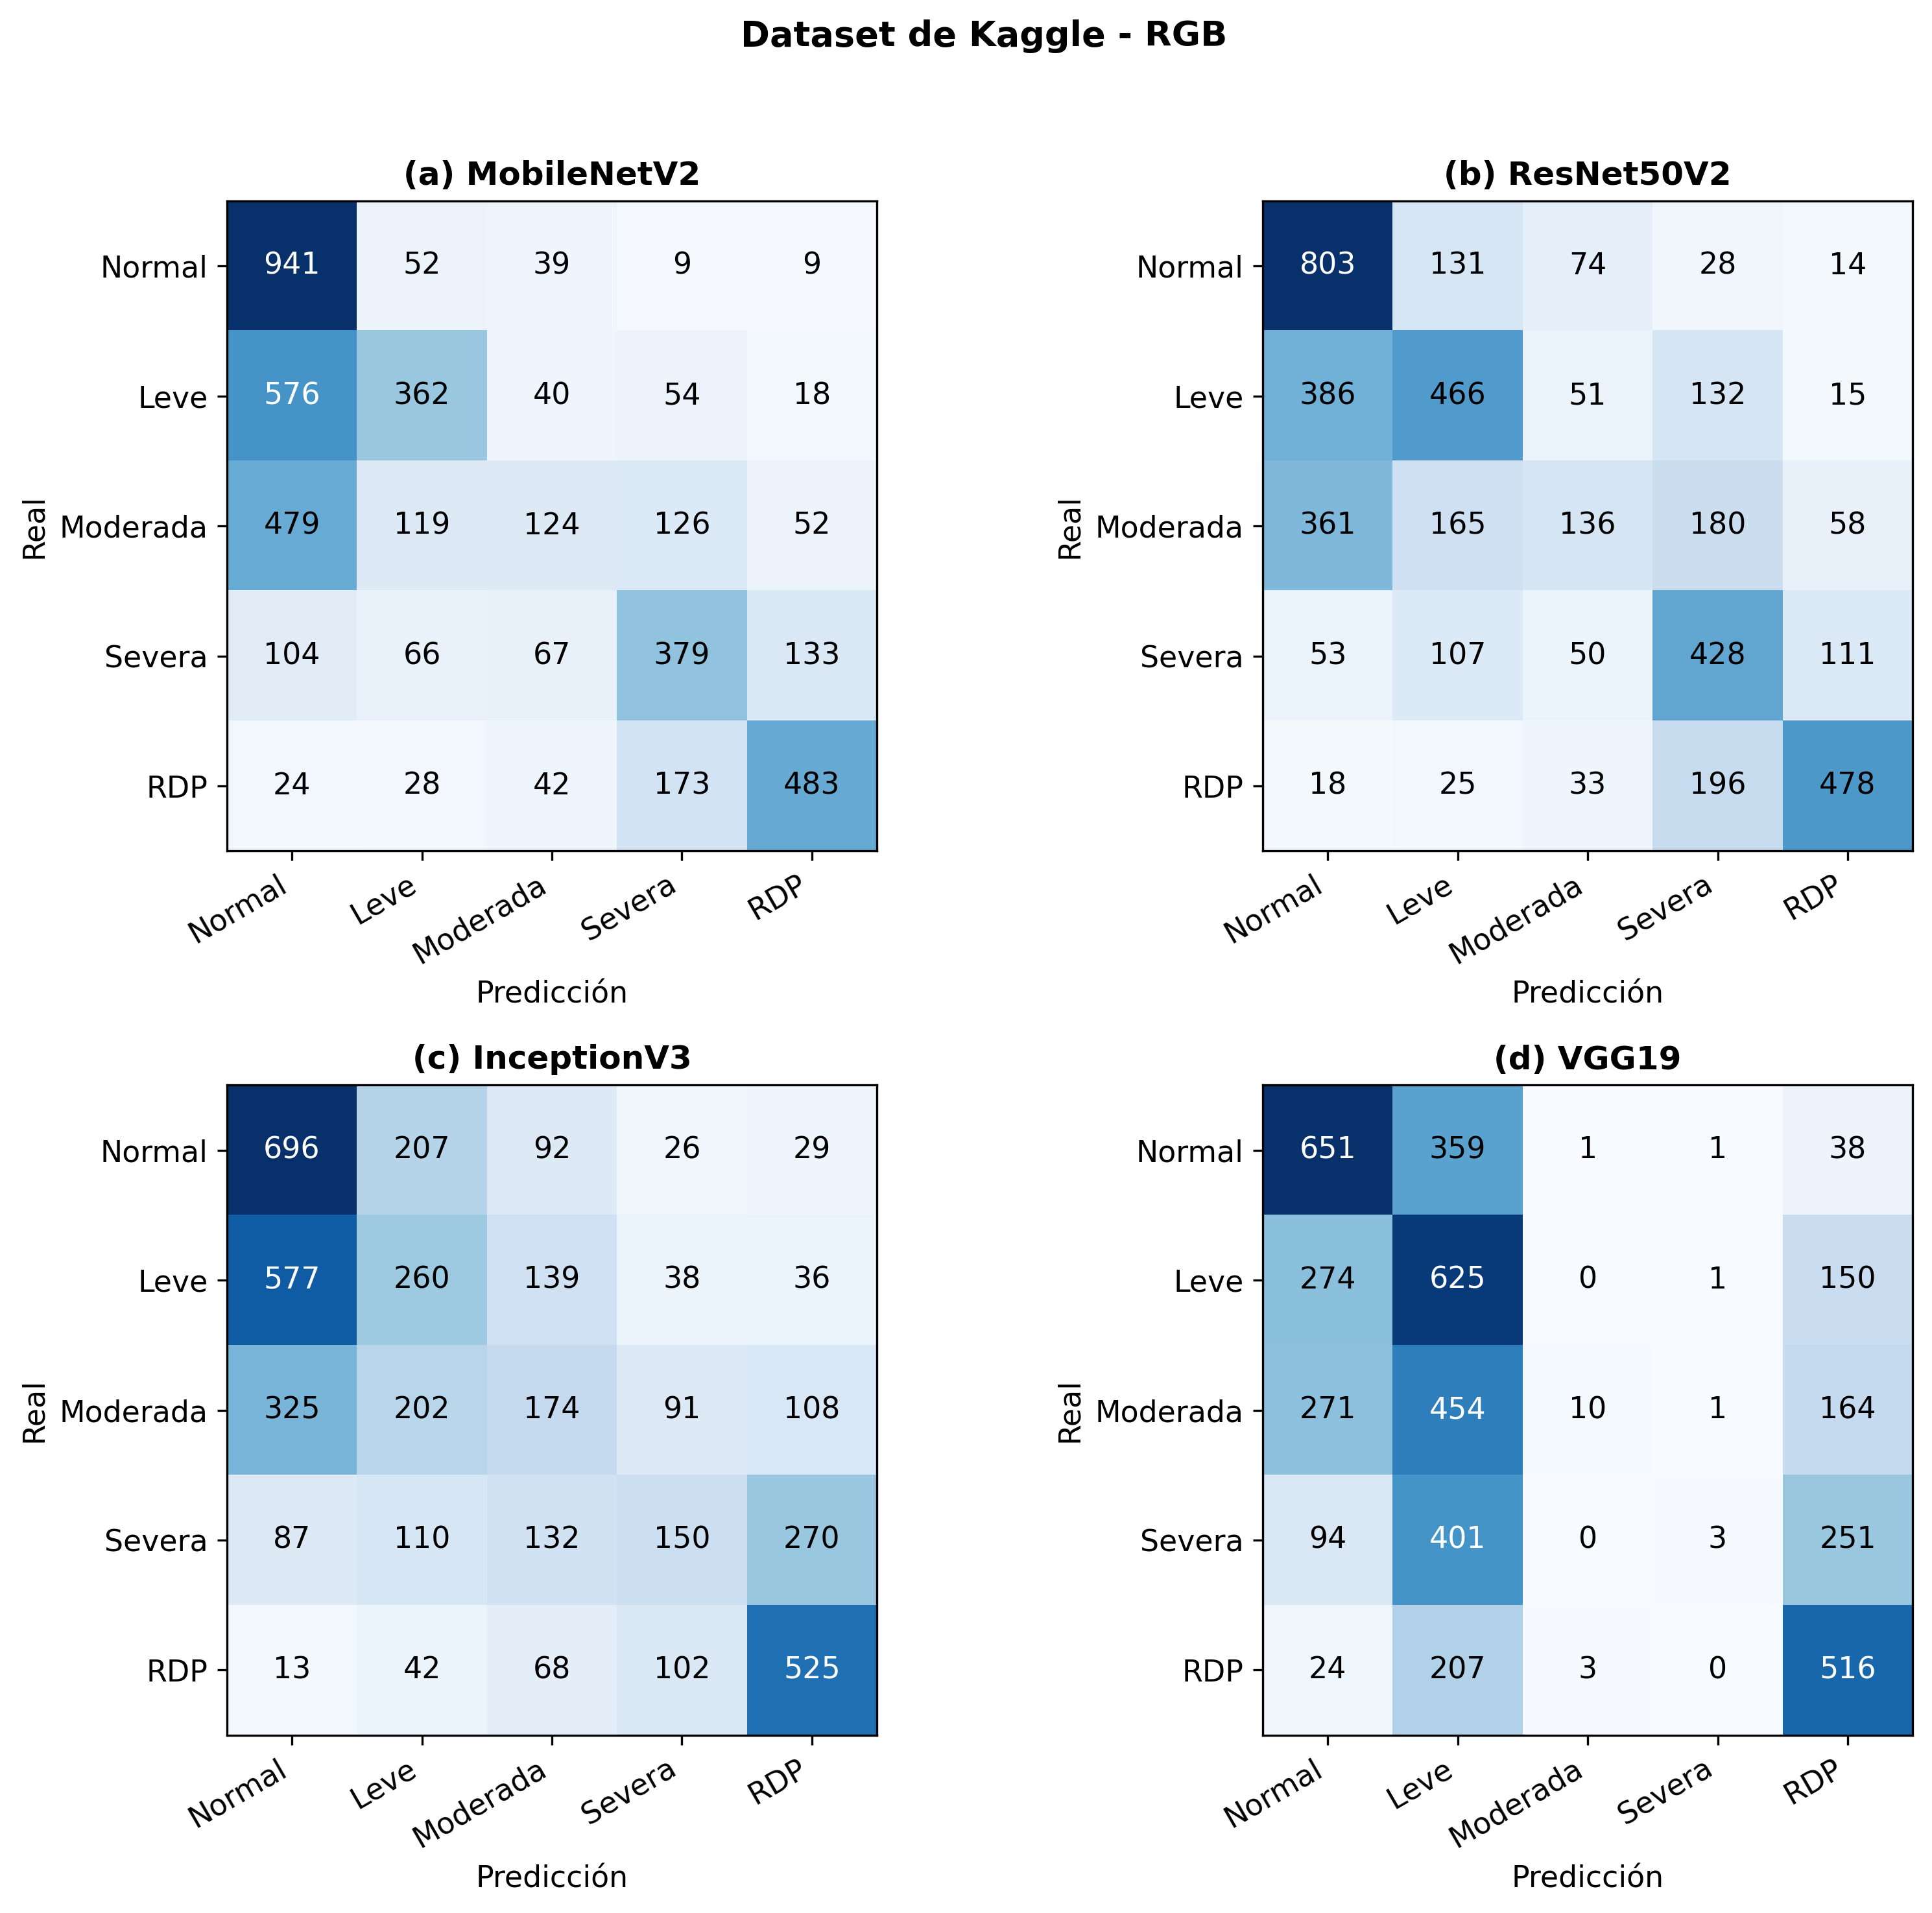
\includegraphics[width=\textwidth]{imágenes/resultados/confusion_multiclase_rgb.png}
	\caption*{\textit{Fuente: Elaboración propia}}
\end{figure}

La Figura~\ref{fig:confusion-multiclase-verde} repite este ejercicio utilizando
únicamente el canal verde como entrada; el lector puede comparar directamente esta
matriz contra la de la Figura~\ref{fig:confusion-multiclase-rgb} para observar el efecto
del canal sobre la distribución de aciertos y errores de cada arquitectura.

\begin{figure}[H]
	\centering
	\caption{Matriz de confusión para la evaluación de cada clasificador multiclase usando el
	dataset de Kaggle canal \textbf{VERDE}}
	\label{fig:confusion-multiclase-verde}
	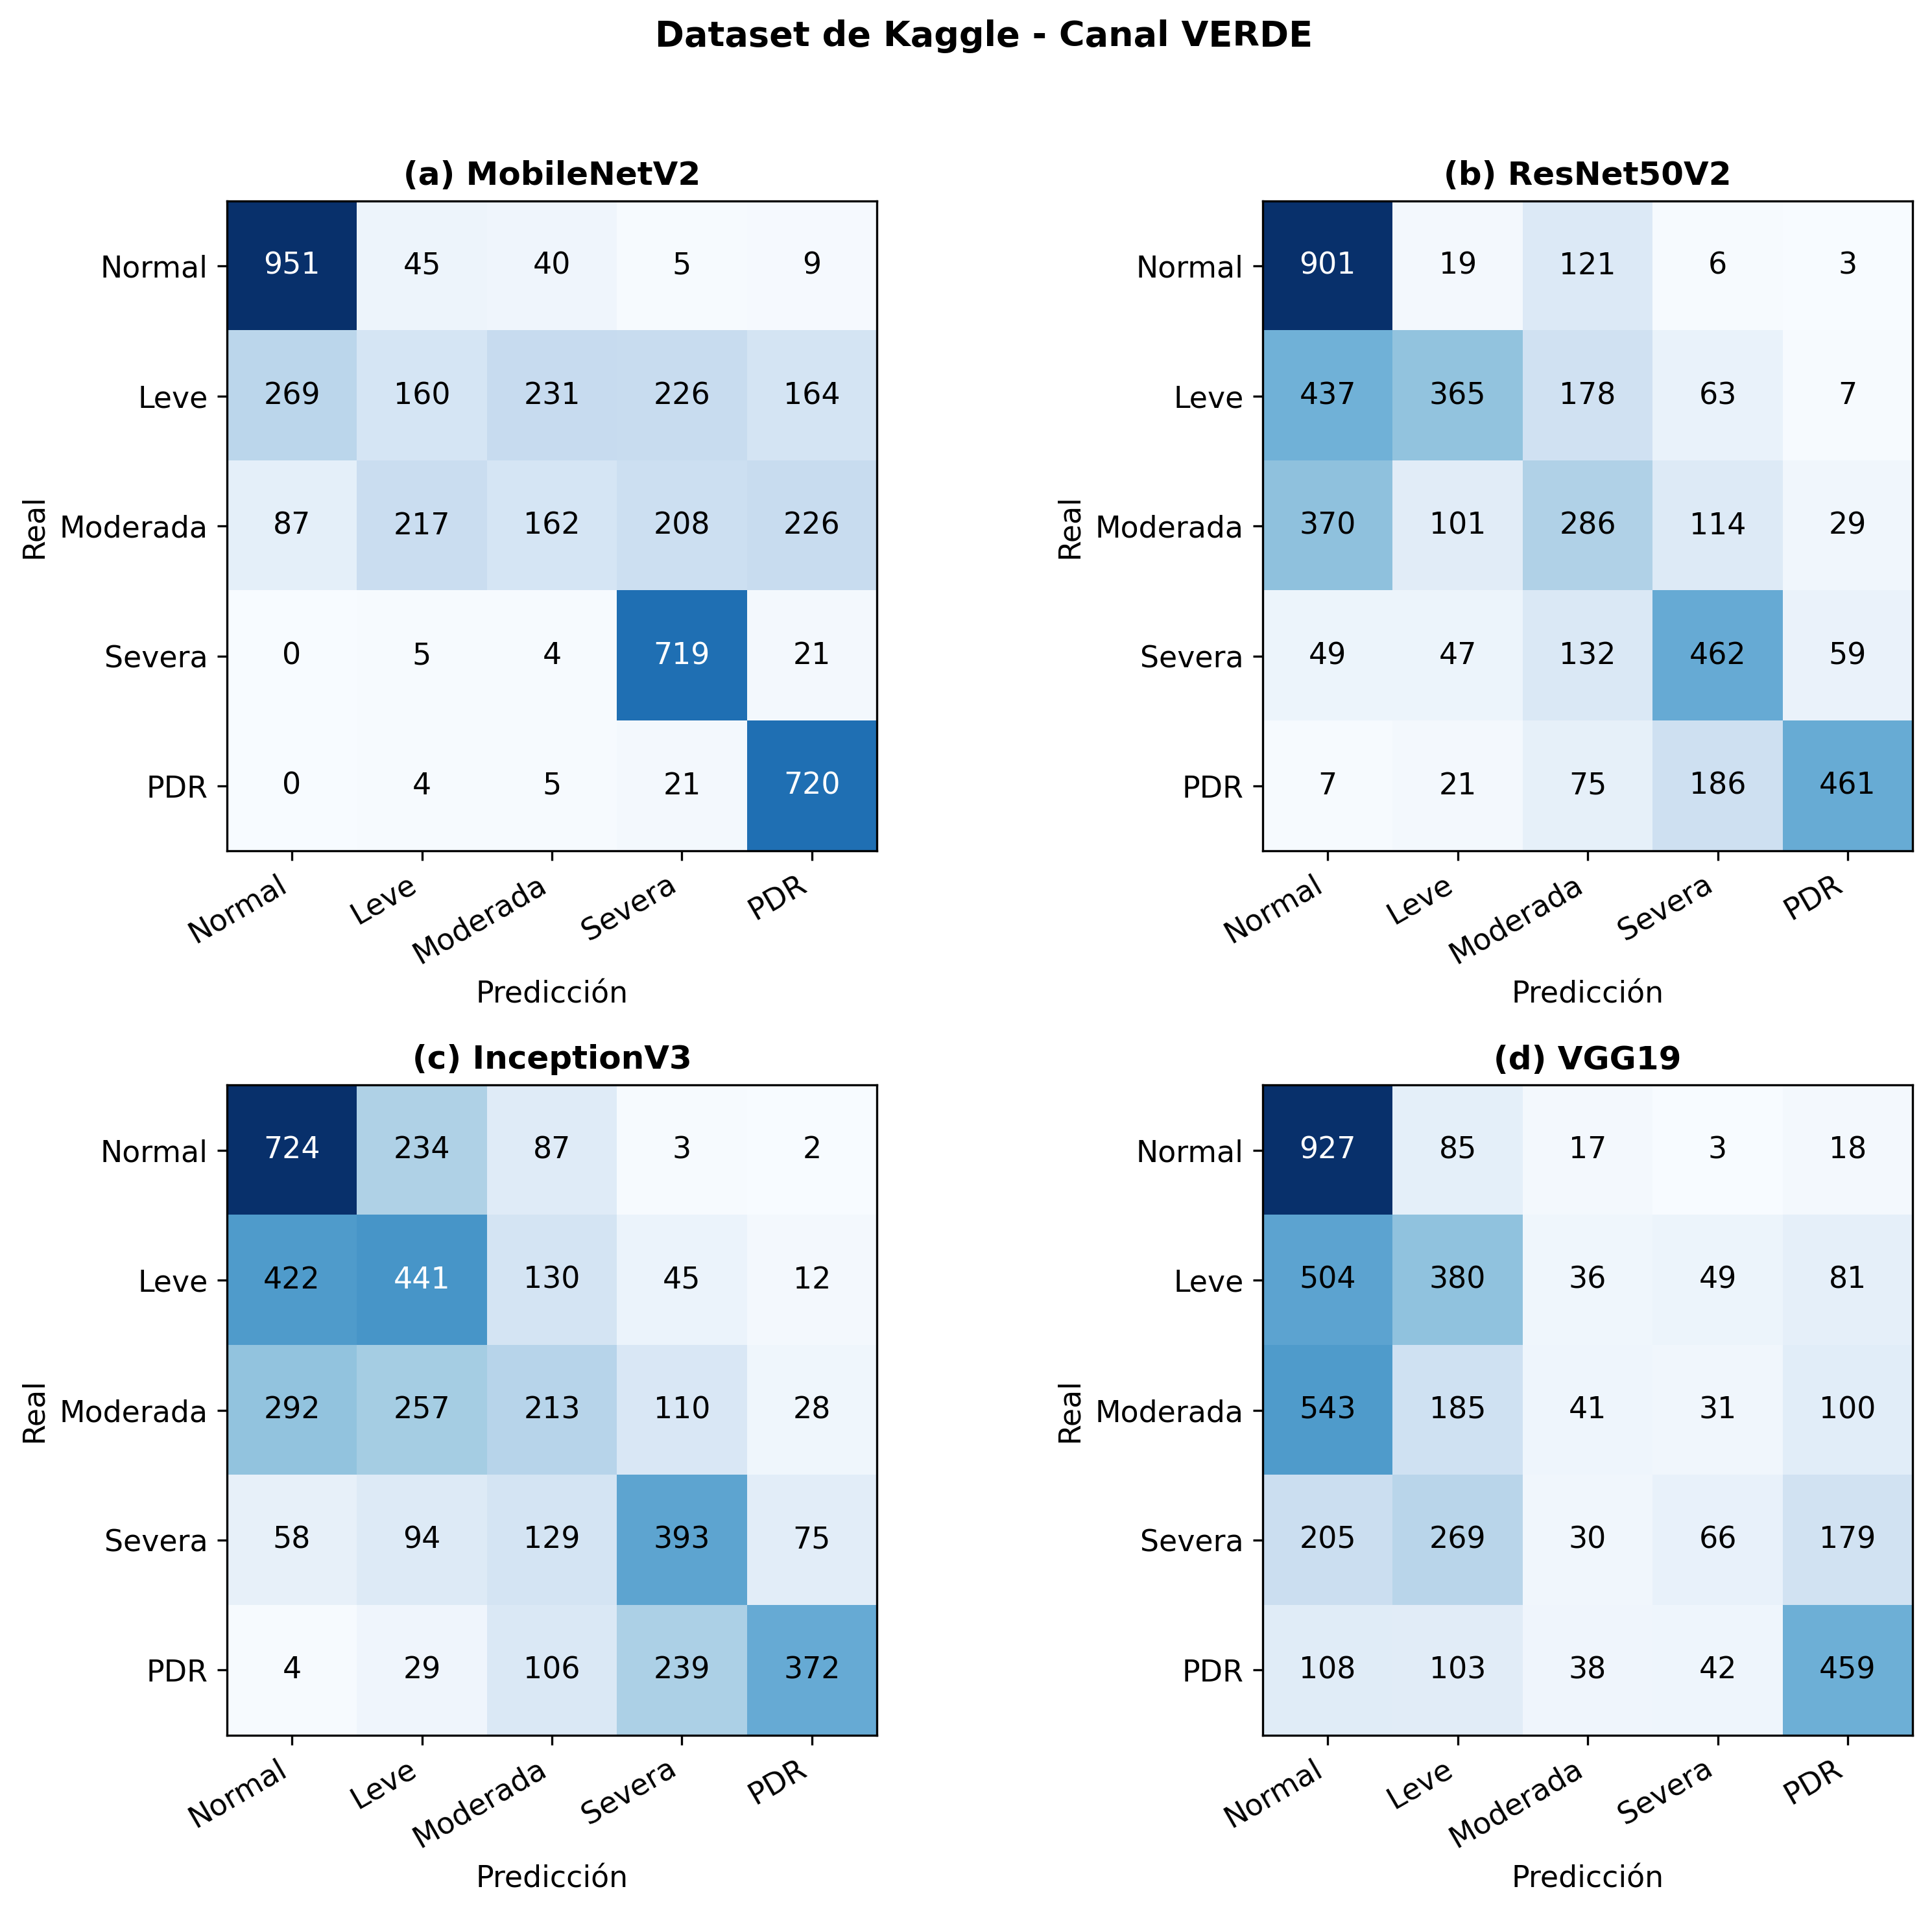
\includegraphics[width=\textwidth]{imágenes/resultados/confusion_multiclase_verde.png}
	\caption*{\textit{Fuente: Elaboración propia}}
\end{figure}

La Figura~\ref{fig:confusion-multiclase-azul} presenta el mismo ejercicio para el canal
azul, uno de los dos canales individuales (junto con el rojo) que obtuvo un desempeño
agregado considerablemente inferior al del canal verde (Sección~
\ref{subsec:analisis-canales}).

\begin{figure}[H]
	\centering
	\caption{Matriz de confusión para la evaluación de cada clasificador multiclase usando el
	dataset de Kaggle canal \textbf{AZUL}}
	\label{fig:confusion-multiclase-azul}
	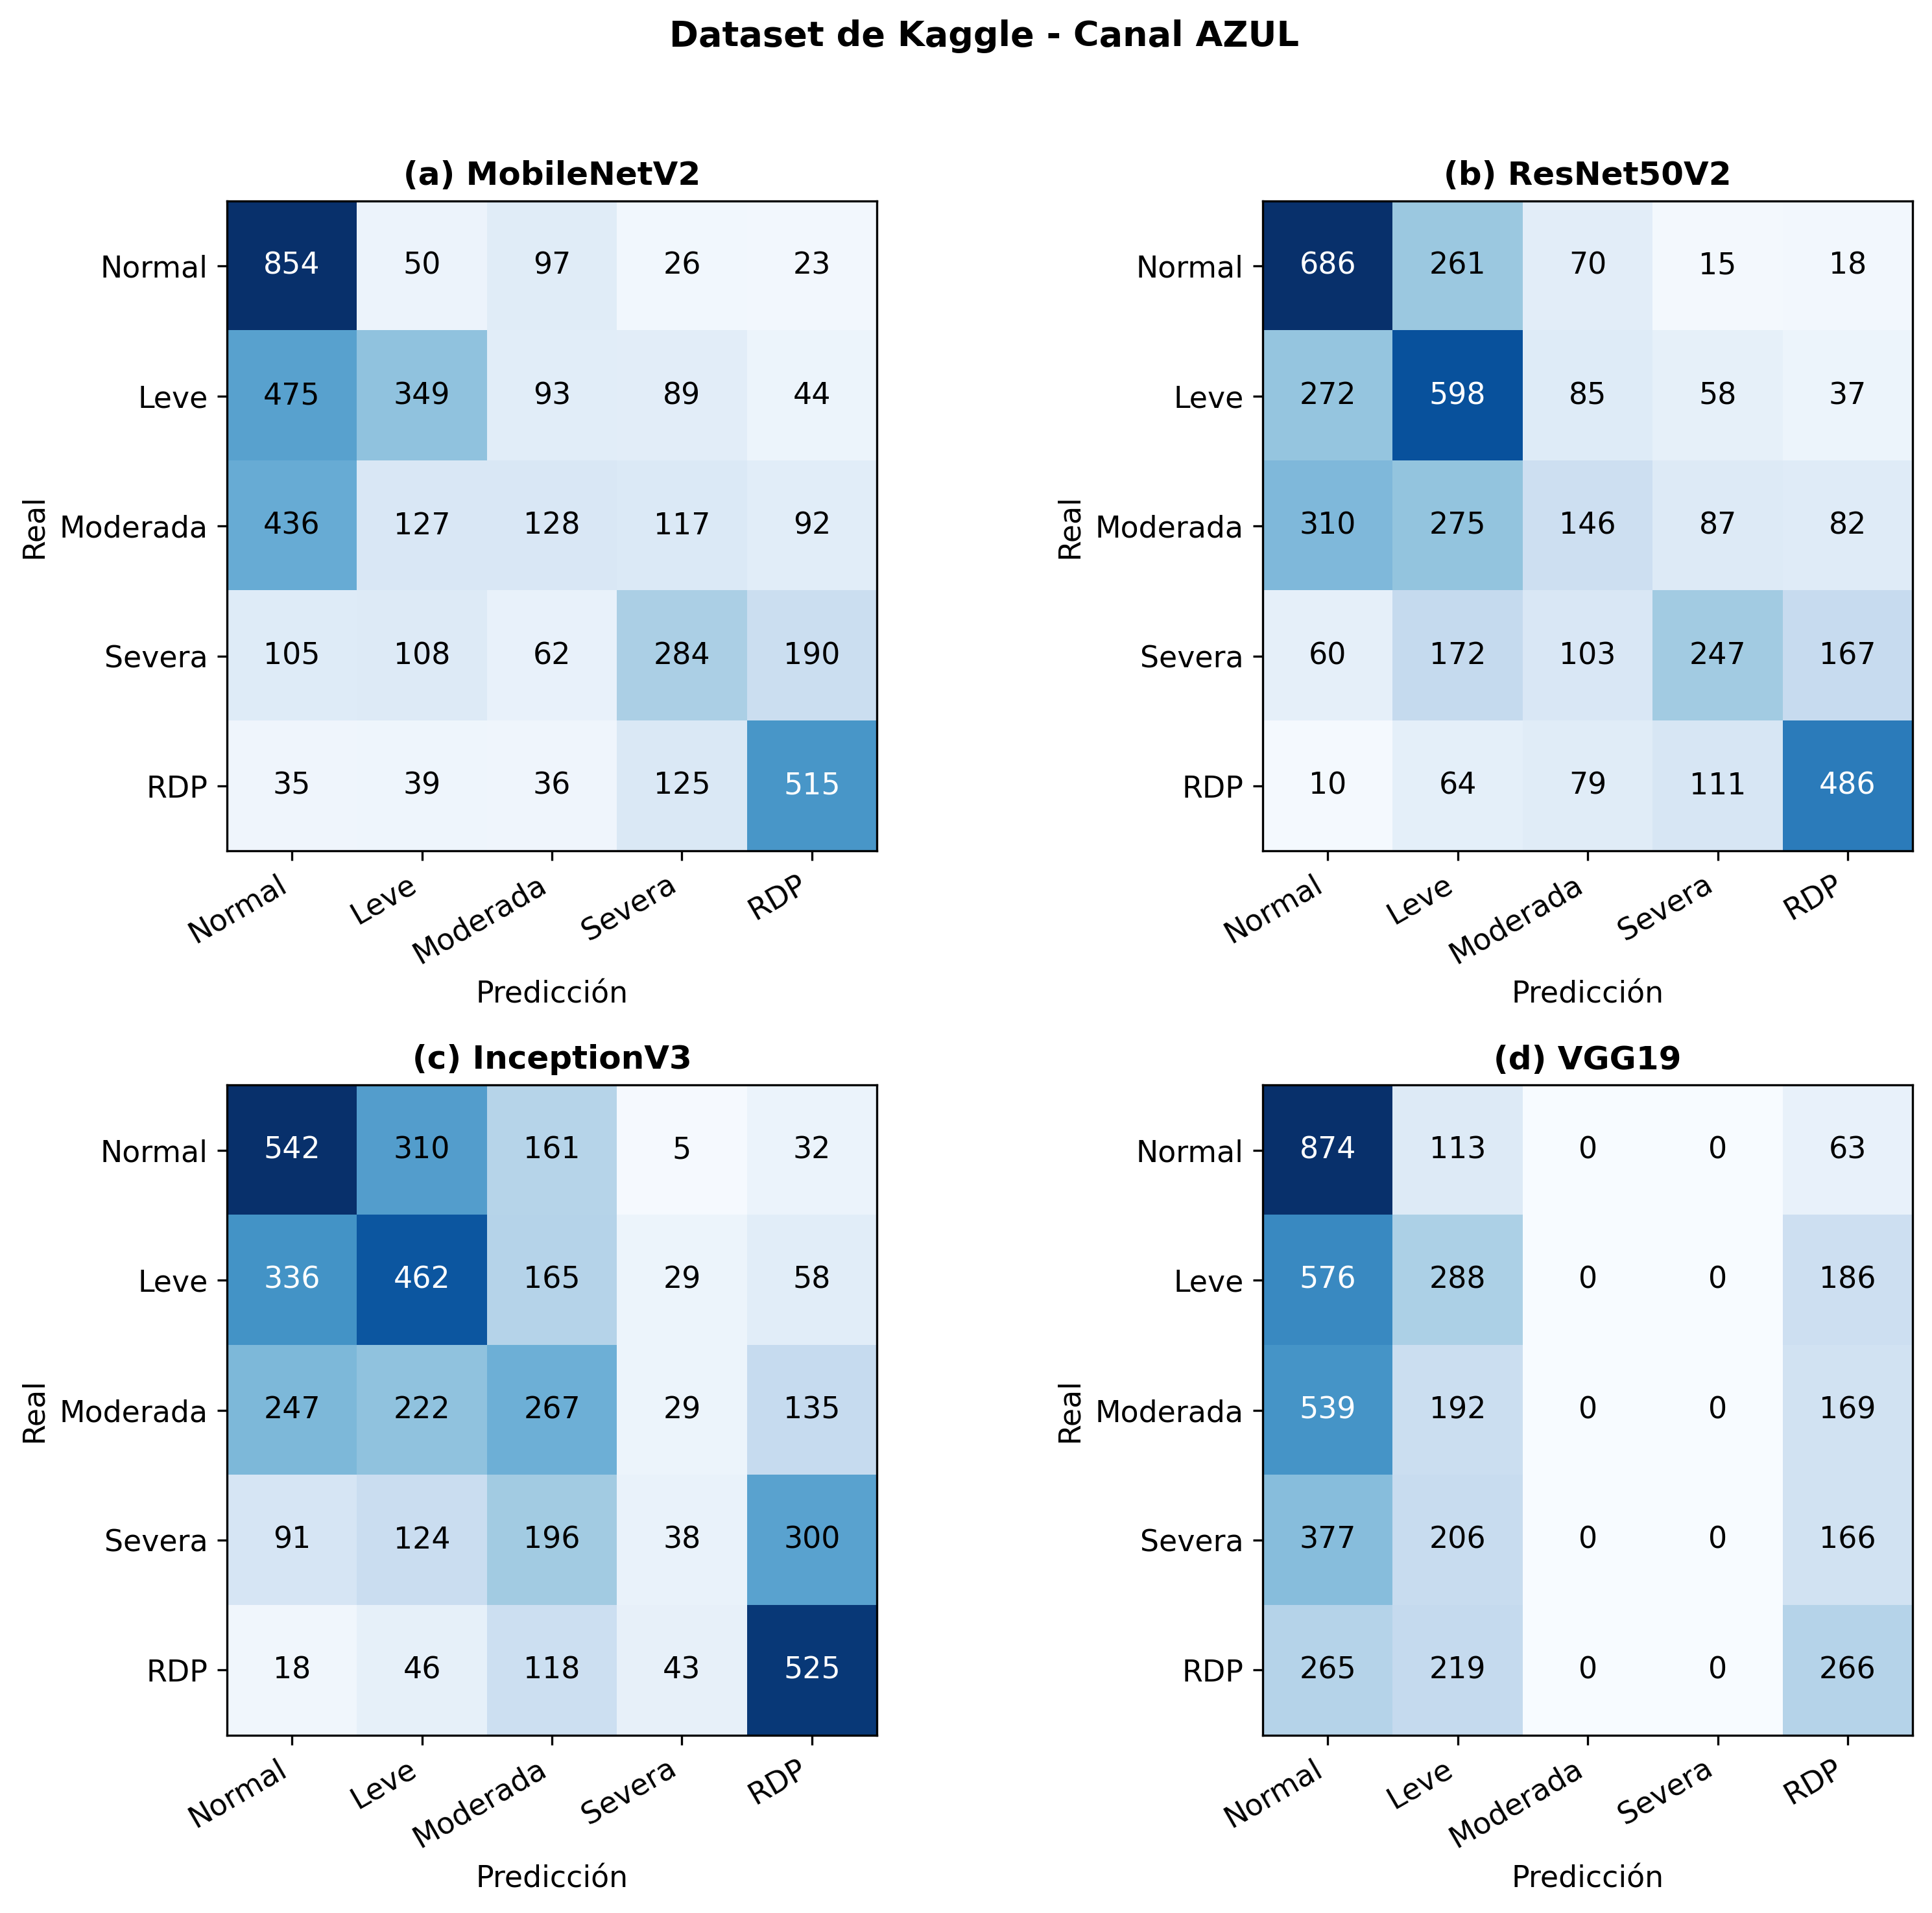
\includegraphics[width=\textwidth]{imágenes/resultados/confusion_multiclase_azul.png}
	\caption*{\textit{Fuente: Elaboración propia}}
\end{figure}

Finalmente, la Figura~\ref{fig:confusion-multiclase-rojo} presenta las matrices de
confusión para el canal rojo, con el cual se completa la comparación de las cuatro
configuraciones de entrada evaluadas.

\begin{figure}[H]
	\centering
	\caption{Matriz de confusión para la evaluación de cada clasificador multiclase usando el
	dataset de Kaggle canal \textbf{ROJO}}
	\label{fig:confusion-multiclase-rojo}
	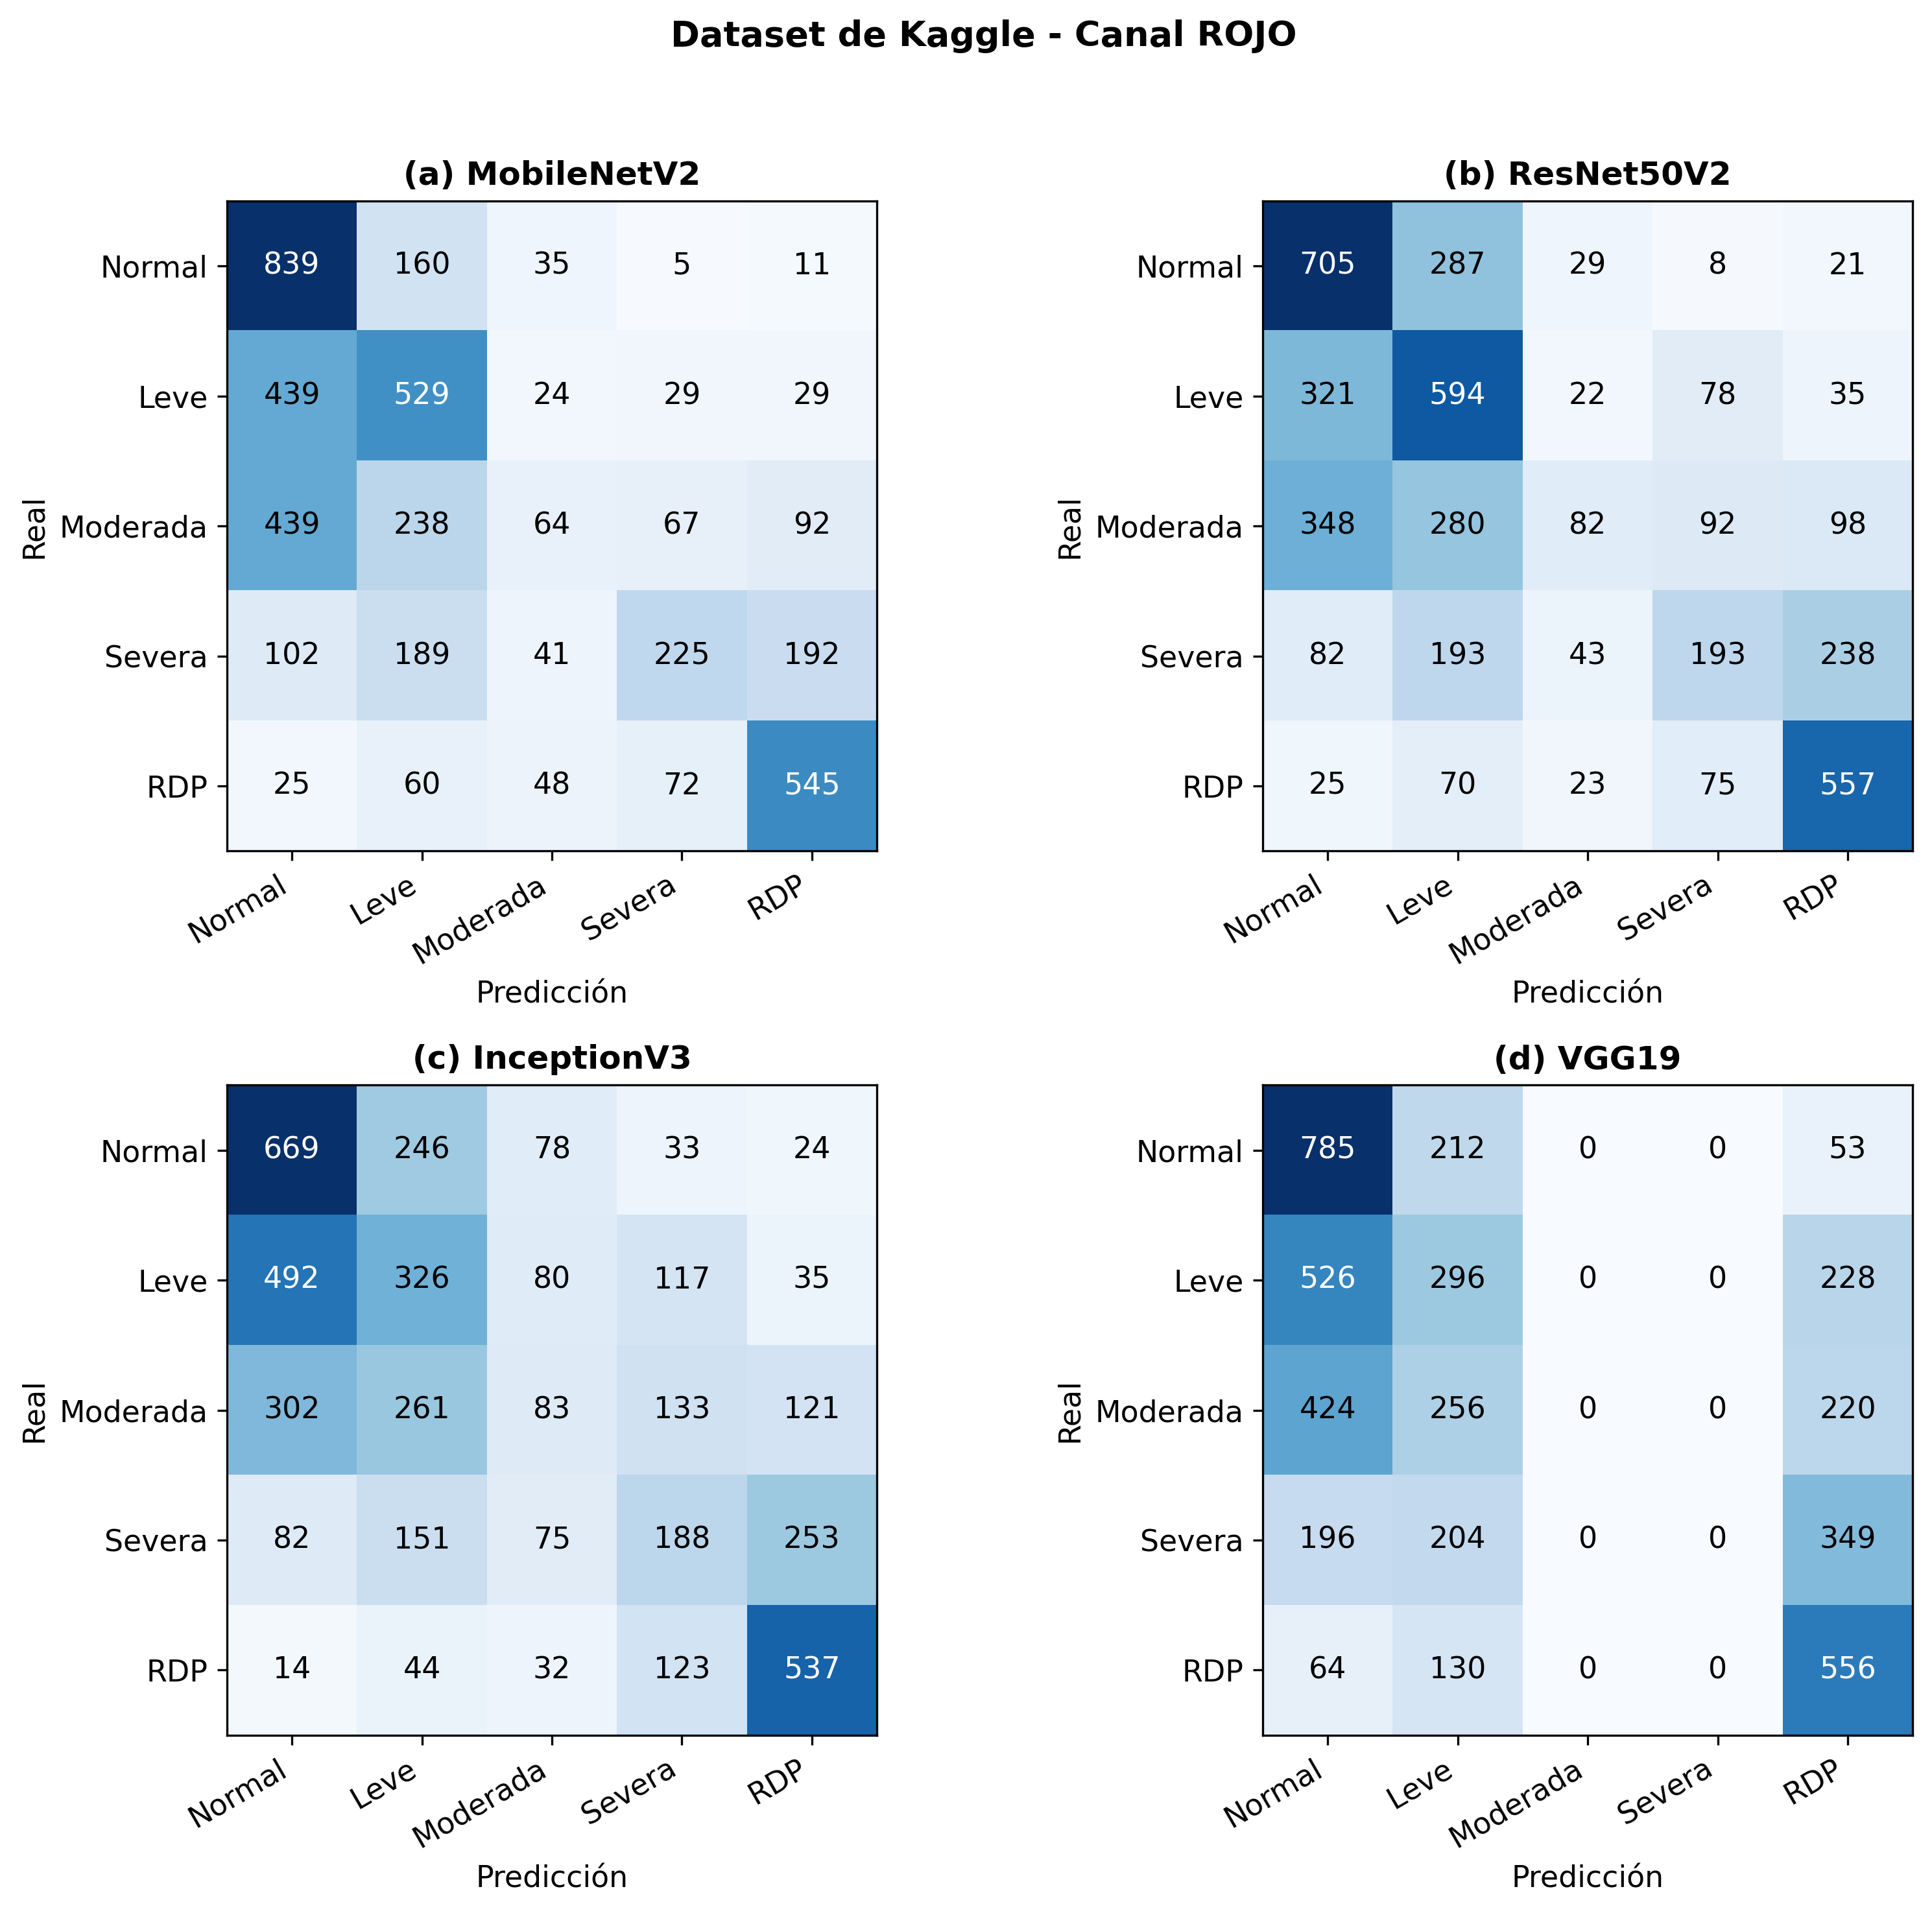
\includegraphics[width=\textwidth]{imágenes/resultados/confusion_multiclase_rojo.png}
	\caption*{\textit{Fuente: Elaboración propia}}
\end{figure}

Para sintetizar estas 16 matrices de confusión en cifras comparables, la
Tabla~\ref{tab:metricas-multiclase-canales} agrega sensibilidad, especificidad,
precisión y F1-score de cada arquitectura para las cuatro configuraciones de entrada; en
ella se observa que MobileNetV2 y ResNet50V2 con el canal verde obtienen el mejor
F1-score (0.54) de toda la comparación, con MobileNetV2 destacándose además por la mayor
sensibilidad (0.65).

\begin{table}[H]
	\centering
	\renewcommand{\arraystretch}{0.8}
	\caption{Desempeño de redes preentrenadas para la clasificación multiclase de
	retinopatía diabética usando todos y cada uno de los canales \textbf{RGB}}
	\label{tab:metricas-multiclase-canales}
	\begin{tabularx}{\textwidth}{l Y Y Y r}
		\toprule
		\multicolumn{5}{c}{RGB} \\
		\midrule
		Red Pre-entrenada  & Sensibilidad & Especificidad &  Precisión & F1-score \\
		\midrule
		MobileNetV2    & 0.55 & 0.87 & 0.52 & 0.50 \\
		ResNet50V2 & 0.51 & 0.88 & 0.51 & 0.49 \\
		InceptionV3& 0.39 & 0.85 & 0.40 & 0.39 \\
		VGG19& 0.38 & 0.85 & 0.50 & 0.31\\
		\multicolumn{5}{c}{Canal rojo} \\
		\midrule
		Red Pre-entrenada  & Sensibilidad & Especificidad &  Precisión & F1-score \\
		\midrule
		MobileNetV2    & 0.48 & 0.87 & 0.48 & 0.45 \\
		ResNet50V2 & 0.47 & 0.87 & 0.46 & 0.43 \\
		InceptionV3& 0.40 & 0.85 & 0.37 & 0.37 \\
		VGG19& 0.35 & 0.84 & 0.21 & 0.26 \\
		\midrule
		\multicolumn{5}{c}{Canal Verde} \\
		\midrule
		Red Pre-entrenada  & Sensibilidad & Especificidad &  Precisión & F1-score \\
		\midrule
		\textbf{MobileNetV2}    & \textbf{0.65} & \textbf{0.89} & \textbf{0.53} & \textbf{0.54} \\
		ResNet50V2 & 0.58 & 0.89 & 0.55 & 0.54 \\
		InceptionV3 & 0.48 & 0.87 & 0.50 & 0.47 \\
		VGG19 & 0.38 & 0.85 & 0.40 & 0.34 \\
		\midrule
		\multicolumn{5}{c}{Canal Azul} \\
		\midrule
		Red Pre-entrenada  & Sensibilidad & Especificidad &  Precisión & F1-score \\
		\midrule
		MobileNetV2    & 0.47 & 0.87 & 0.46 & 0.44 \\
		ResNet50V2 & 0.48 & 0.87 & 0.46 & 0.46 \\
		InceptionV3& 0.41 & 0.85 & 0.38 & 0.38 \\
		VGG19& 0.29 & 0.82 & 0.19 & 0.22 \\
		\bottomrule
	\end{tabularx}
	\caption*{\textit{Fuente: Elaboración propia}}
\end{table}

Más allá de identificar cuál configuración obtiene el mayor F1-score puntual, es posible
cuantificar la magnitud de la ventaja del canal verde promediando su efecto en las cuatro
arquitecturas. La Tabla~\ref{tab:mejora-canal-verde} muestra que, en promedio, el canal
verde mejora el F1-score en +0.05 puntos (+11.8\%) respecto a la imagen RGB completa, en
+0.095 puntos (+25.2\%) respecto al canal rojo y en +0.0975 puntos (+26.0\%) respecto al
canal azul. La ventaja es consistente en las cuatro arquitecturas evaluadas: incluso en el
caso menos favorable (MobileNetV2 frente a RGB) el canal verde aporta una mejora de
+8.0\%, mientras que en el caso más favorable (VGG19 frente al canal azul) la mejora
relativa alcanza +54.5\%, aunque este último valor debe interpretarse con cautela porque
la configuración VGG19-azul corresponde a un modelo colapsado que nunca predice las clases
Moderada ni Severa (Figura~\ref{fig:confusion-multiclase-azul}, panel d). En términos de
sensibilidad el patrón se repite: el canal verde promedia 0.52 frente a 0.46 de RGB
(+14.2\%), 0.43 de rojo (+22.9\%) y 0.41 de azul (+26.7\%).

\begin{table}[H]
	\centering
	\caption{Mejora del canal verde frente a las demás configuraciones de entrada en
	F1-score (clasificación multiclase)}
	\label{tab:mejora-canal-verde}
	\begin{tabularx}{\textwidth}{l Y Y Y}
		\toprule
		Red Pre-entrenada & $\Delta$F1 vs. RGB & $\Delta$F1 vs. Rojo & $\Delta$F1 vs. Azul \\
		\midrule
		MobileNetV2 & +0.04 (+8.0\%) & +0.09 (+20.0\%) & +0.10 (+22.7\%) \\
		ResNet50V2  & +0.05 (+10.2\%) & +0.11 (+25.6\%) & +0.08 (+17.4\%) \\
		InceptionV3 & +0.08 (+20.5\%) & +0.10 (+27.0\%) & +0.09 (+23.7\%) \\
		VGG19       & +0.03 (+9.7\%) & +0.08 (+30.8\%) & +0.12 (+54.5\%) \\
		\midrule
		\textbf{Promedio} & \textbf{+0.05 (+11.8\%)} & \textbf{+0.095 (+25.2\%)} & \textbf{+0.0975 (+26.0\%)} \\
		\bottomrule
	\end{tabularx}
	\caption*{\textit{Fuente: Elaboración propia. El promedio se calcula como la diferencia
	entre las medias de F1-score de las cuatro arquitecturas para cada configuración.}}
\end{table}

Esta ventaja no se distribuye de manera uniforme entre las cinco clases, sino que se
concentra en las categorías definidas clínicamente por una mayor densidad de lesiones
hemorrágicas y microvasculares. Según los criterios de severidad de la escala ICDR, la
retinopatía severa (RD3) se distingue de la moderada por un incremento sustancial en el
conteo de hemorragias intrarretinianas, anomalías microvasculares intrarretinianas (IRMA)
y arrosariamiento venoso, lesiones que, de acuerdo con el principio de absorción
diferencial de la hemoglobina citado anteriormente \myfootcite{pao2020bichannel}, son
precisamente las que el canal verde realza. Calculando la sensibilidad por clase a partir
de las matrices de confusión ya presentadas (Figuras~\ref{fig:confusion-multiclase-rgb} a
\ref{fig:confusion-multiclase-rojo}), se observa que para la clase Severa el canal verde
eleva la sensibilidad de MobileNetV2 de 0.51 (RGB) a 0.57, frente a apenas 0.30 con el
canal rojo (+90\% relativo) y 0.38 con el canal azul (+50\% relativo); en ResNet50V2 el
efecto es aún más marcado, con una sensibilidad de 0.62 para el canal verde frente a 0.57
(RGB), 0.26 (rojo, +139\% relativo) y 0.33 (azul, +88\% relativo). Este patrón respalda la
hipótesis de que la ventaja del canal verde no es un artefacto estadístico, sino que
responde a una mejor representación de las lesiones que definen clínicamente la severidad
de la enfermedad.

Cabe señalar que esta ventaja no se extiende de forma uniforme a la clase PDR (RD4): en
ambas arquitecturas el canal rojo iguala o supera al verde en la sensibilidad de esta
categoría (0.73 frente a 0.67 en MobileNetV2 y 0.74 frente a 0.61 en ResNet50V2), lo cual
sugiere
que en la etapa proliferativa la vasculatura de neoformación, capturada con mayor
contraste por el canal rojo, aporta información complementaria que el canal verde no
logra representar igual de bien. En conjunto, estos resultados matizan la ventaja del
canal verde: es consistente y cuantificable en el desempeño agregado y particularmente
pronunciada en la clase Severa, pero no representa una superioridad absoluta en todas las
categorías clínicas.


 
\chapter{DISCUSIÓN} \label{chap:discusion}

Los resultados experimentales obtenidos en este trabajo muestran que los modelos basados
en redes neuronales convolucionales con aprendizaje por transferencia constituyen una
alternativa viable para la detección automatizada de retinopatía diabética en imágenes
del fondo de ojo. A continuación se interpretan los hallazgos más relevantes,
contrastándolos con el marco teórico y con investigaciones previas en el área.

\section{Desempeño del clasificador binario y comparación con la literatura}

El modelo MobileNetV2 con filtrado y umbral óptimo alcanzó una sensibilidad de 96.5\% y
un F1-score de 0.96 en el conjunto de prueba interno, métricas que lo posicionan
favorablemente frente a trabajos previos. Gulshan et al. reportaron una sensibilidad del
97.5\% utilizando arquitecturas más profundas entrenadas con conjuntos de datos
considerablemente mayores \myfootcite{gulshan2016development}, lo cual sugiere que la
estrategia de preprocesamiento implementada en este trabajo logró compensar parcialmente
las limitaciones en volumen de datos mediante la mejora de la calidad de las
características visuales extraídas.

Es importante precisar el alcance de las siguientes explicaciones: este trabajo compara
arquitecturas completas entre sí y no realiza experimentos de ablación que aíslen la
contribución individual de cada componente arquitectónico al desempeño observado. Por
ello, las relaciones entre características de diseño y desempeño que se plantean a
continuación deben entenderse como interpretaciones posibles, sustentadas en literatura
previa, y no como causas demostradas experimentalmente por este trabajo.

Una interpretación posible de la superioridad de MobileNetV2 sobre las demás
arquitecturas evaluadas (VGG19, ResNet50V2 e InceptionV3) se relaciona con
características propias de su diseño. Los bloques residuales invertidos de MobileNetV2,
que emplean convoluciones separables en profundidad junto con cuellos de botella
lineales, se han asociado con una forma de regularización implícita que podría resultar
beneficiosa cuando el conjunto de datos disponible es limitado
\myfootcite{sandler2018mobilenetv2}, lo que ofrece una posible explicación de por qué
este modelo mostró menor propensión al sobreajuste que arquitecturas más grandes en este
experimento. De manera similar, se ha planteado que la ausencia de activaciones no
lineales en las capas de proyección ayuda a preservar información de baja
dimensionalidad \myfootcite{sandler2018mobilenetv2}, lo cual podría ser relevante para
capturar características sutiles como las lesiones microvasculares en etapas tempranas de
la RD, aunque este trabajo no verificó dicho mecanismo de forma directa.

Los resultados contrastan con el desempeño de VGG19, que a pesar de su profundidad y
capacidad de extracción de características, mostró métricas inferiores (F1-score de 0.86
sin filtrado). Una posible explicación es que esta arquitectura, caracterizada por un
elevado número de parámetros en sus capas completamente conectadas y la ausencia de
conexiones residuales, sea más propensa al sobreajuste en este escenario de datos
limitados; sin embargo, este trabajo no midió directamente el grado de sobreajuste de
cada modelo (por ejemplo, mediante la brecha entre error de entrenamiento y validación),
por lo que esta explicación permanece como hipótesis. Es consistente, en todo caso, con
lo reportado por Kandel y Castelli, quienes identificaron que arquitecturas más compactas
tienden a generalizar mejor en dominios médicos con datos limitados
\myfootcite{kandel2020transfer}.

\section{Impacto del preprocesamiento en el rendimiento del modelo}

La implementación del algoritmo de filtrado, que incluyó normalización del color mediante
sustracción del promedio local con filtro gaussiano y recorte del fondo oscuro de la
imagen, produjo mejoras consistentes en todas las arquitecturas evaluadas. El incremento
del F1-score de 0.95 a 0.96 en MobileNetV2, aunque aparentemente modesto, se acompañó de
una reducción de falsos positivos (de 6 a 4 casos) y de falsos negativos (de 5 a 3 casos),
con implicaciones clínicas relevantes al disminuir tanto las derivaciones innecesarias
como los casos de RD no detectados en un escenario de tamizaje.

Este resultado es consistente con la importancia del preprocesamiento destacada en la
revisión de literatura: Tabtaba y Ata reportaron mejoras similares al aplicar técnicas de
ecualización adaptativa del histograma sobre imágenes de fondo de ojo
\myfootcite{tabtaba2024diabetic}. La normalización de color implementada en este trabajo
busca mitigar las variaciones de brillo y contraste inherentes a la captura de imágenes
en entornos clínicos heterogéneos, donde las condiciones de iluminación y los equipos de
adquisición varían considerablemente; el recorte del fondo oscuro, por su parte, elimina
regiones no informativas que podrían introducir ruido en el proceso de extracción de
características.

\section{Validación externa y capacidad de generalización}

La evaluación del modelo en conjuntos de datos externos (FOSCAL, IDRiD y MESSIDOR-2)
mostró un desempeño variable según el conjunto, con una disminución en las métricas
respecto al conjunto de prueba interno de Kaggle (Sección~\ref{subsec:validacion-externa}).
Este hallazgo —una caída de desempeño al evaluar fuera del dominio de entrenamiento— no
es particular de este trabajo: es un fenómeno documentado en la literatura reciente sobre
generalización cruzada de modelos de clasificación de RD. Hashmi reporta, por ejemplo,
una caída de sensibilidad para RD referible de 0.879 en el dominio de entrenamiento
(APTOS) a 0.620 al evaluar sobre MESSIDOR-2 sin reentrenamiento, señalando que las
métricas en dominio tienden a sobreestimar el desempeño real desplegable
\myfootcite{hashmi2026crossdomain}. Este patrón resulta relevante para interpretar por
qué el desempeño de este trabajo también varía entre datasets externos.

Las diferencias entre FOSCAL, IDRiD y MESSIDOR-2 no se limitan a la calidad visual de las
imágenes: involucran distinto modelo de cámara, resolución, protocolo de captura y
población de origen (india, francesa y colombiana, respectivamente; véase la
Sección~\ref{sec:conjuntos-datos}), factores que la literatura sobre cambio de dominio
identifica como determinantes de la transferibilidad de un modelo entrenado en un dominio
distinto \myfootcite{hashmi2026crossdomain}. Dado que estas variables no fueron
controladas ni desagregadas en el análisis, no es posible atribuir con precisión qué
proporción de la variación observada corresponde a cada factor; esto se reconoce como
limitación en la Sección~\ref{sec:limitaciones-discusion}.

En conjunto, estos resultados sugieren que el modelo mantiene un desempeño razonable
fuera del dominio de entrenamiento, comparable en magnitud a la caída reportada en
trabajos similares, pero no permiten afirmar una capacidad de generalización robusta o
universal: como en el caso documentado por Hashmi, las métricas del conjunto de
entrenamiento tienden a sobreestimar el desempeño esperable en un despliegue real, y una
conclusión más definitiva requeriría aislar el efecto de cada fuente de variación entre
datasets \myfootcite{hashmi2026crossdomain}.

\section{Análisis del clasificador multiclase y el efecto del canal de color}

Los experimentos de clasificación multiclase revelaron hallazgos relevantes respecto al
procesamiento del color en imágenes de fondo de ojo. El canal verde demostró
consistentemente el mejor desempeño (exactitud de 0.55, sensibilidad promedio de 0.56),
superando tanto a la imagen RGB completa (+11.8\% en F1-score promedio de las cuatro
arquitecturas evaluadas) como a los canales rojo (+25.2\%) y azul (+26.0\%) de manera
individual (Tabla~\ref{tab:mejora-canal-verde}). Esta ventaja se concentra
particularmente en la clase Severa (RD3), donde la sensibilidad obtenida con el canal
verde supera en más de 85\% a la del canal rojo y en más de 50\% a la del canal azul en las dos
arquitecturas de mejor desempeño (Sección~\ref{subsec:analisis-canales}). Este resultado
tiene fundamento fisiológico: el canal verde proporciona mejor contraste para la
visualización de estructuras vasculares y lesiones hemorrágicas debido a la absorción
diferencial de la hemoglobina en esta longitud de onda, el mismo principio que sustenta
el uso clínico histórico de filtros verdes en oftalmoscopia para realzar hemorragias y
exudados \myfootcite{pao2020bichannel}. Los microaneurismas, hemorragias y anomalías
microvasculares intrarretinianas, signos que definen clínicamente la etapa severa de la
retinopatía diabética, presentan mayor visibilidad en este espectro cromático, lo que es
consistente con la ganancia de sensibilidad observada precisamente en esa clase. La ventaja no
es, sin embargo, absoluta: en la clase PDR (RD4), asociada a la neoformación vascular, el
canal rojo iguala o supera al verde, lo que sugiere que ningún canal individual captura
por sí solo toda la información relevante en las etapas más avanzadas de la enfermedad.

Este hallazgo es consistente con la literatura disponible sobre análisis de canales
individuales en RD, aunque dicha literatura resulta comparativamente escasa
(Sección~\ref{chap:trabajos-previos}). Pao et al. reportaron mejoras en la detección de
RD al extraer específicamente el canal verde para el cálculo de características de
entropía, superando el desempeño obtenido con la imagen en escala de grises
\myfootcite{pao2020bichannel}. Singh, Gupta y Dung, en un estudio que comparó canales
individuales de forma más directa, también encontraron diferencias de desempeño entre
canales, aunque limitado a una sola arquitectura y sin un análisis sistemático a través de
múltiples redes preentrenadas \myfootcite{singh2024finetuned}. El presente trabajo amplía
esta evidencia al comparar los cuatro canales (RGB, rojo, verde y azul) de forma
sistemática sobre cuatro arquitecturas distintas en un escenario multiclase, lo que
sustenta de manera más generalizable la ventaja del canal verde reportada previamente.

La dificultad persistente en la clasificación de las clases RD2 (moderada) y RD3 (severa)
observada en todos los experimentos constituye un hallazgo relevante. La sensibilidad
para RD2 fue consistentemente la más baja (valores entre 0.01 y 0.31 dependiendo de la
configuración), lo cual sugiere que las características distintivas de esta categoría no
quedan suficientemente representadas en las arquitecturas empleadas. Desde la perspectiva
clínica, la retinopatía diabética moderada representa una etapa de transición
caracterizada por la presencia de más microaneurismas que la etapa leve, pero sin
alcanzar los criterios que definen la etapa severa. Esta naturaleza transicional, con
límites difusos entre categorías adyacentes, explica en parte la confusión observada en
las matrices de confusión.

Este fenómeno de confusión entre clases intermedias ha sido documentado en trabajos
previos: Gayathri et al. reportaron dificultades similares en la discriminación de etapas
moderadas, proponiendo el uso de clasificadores en cascada o características multiescala
como estrategias de mitigación \myfootcite{gayathri2021diabetic}. Los resultados
obtenidos sugieren que futuras investigaciones podrían explorar técnicas específicas para
abordar este desafío, incluyendo funciones de pérdida focal que penalicen más severamente
los errores en clases difíciles, aumento de datos específico para clases intermedias, o
mecanismos de atención que enfoquen el análisis en regiones anatómicas específicas donde
las lesiones discriminantes tienden a manifestarse.

\section{Justificación de las decisiones arquitectónicas}

La configuración del clasificador, que incorpora bloques Multi-Head Attention posteriores
al extractor de características y capas GaussianNoise entre las capas densas, responde a
consideraciones específicas del dominio de aplicación. Los mecanismos de atención
permiten al modelo ponderar diferencialmente las regiones del mapa de características, lo
cual resulta particularmente relevante en imágenes de fondo de ojo donde las lesiones
ocupan fracciones pequeñas del área total de la imagen; esta capacidad de enfoque
selectivo, documentada en trabajos como el de Dosovitskiy et al.
\myfootcite{dosovitskiy2020image}, complementa la extracción de características locales
realizada por las capas convolucionales con información de contexto global.

La inyección de ruido gaussiano durante el entrenamiento actúa como regularizador
estocástico que expone al modelo a versiones perturbadas de las activaciones internas.
Esta estrategia, respaldada por los estudios de Zur et al., simula la variabilidad
inherente a la adquisición de imágenes médicas (diferencias en iluminación, ruido del
sensor, artefactos de preprocesamiento), forzando al clasificador a aprender
representaciones robustas que no dependan de valores exactos de activación
\myfootcite{zur2009noise}.

La selección de la función de activación ReLU para capas intermedias y Softmax para la
capa de salida sigue prácticas establecidas en la literatura. Asadi y Jiang demostraron
que esta combinación posee propiedades de aproximación universal, proporcionando
fundamento teórico a su amplia adopción empírica \myfootcite{asadi2020approximation}.
Además, la función Softmax garantiza que las salidas del clasificador multiclase
constituyan una distribución de probabilidad válida, facilitando la interpretación
clínica de las predicciones y la implementación de umbrales de confianza para casos que
requieran revisión por especialistas.

\section{Análisis de errores e implicaciones clínicas}

El análisis de las matrices de confusión revela patrones de error con implicaciones
clínicas diferenciadas. En el clasificador binario, la proporción de falsos negativos
(casos de RD no detectados) se mantuvo baja en las configuraciones con mejor desempeño
(3 a 5 casos sobre aproximadamente 105 por clase), lo cual es relevante en un contexto de
tamizaje donde la prioridad es maximizar la detección de casos que requieren atención
especializada. Los falsos positivos, aunque implican derivaciones innecesarias con su
correspondiente costo para el sistema de salud, no conllevan el riesgo de progresión de
la enfermedad asociado a los casos no detectados; esta asimetría de costos clínicos es la
que sustenta la priorización de la sensibilidad discutida en la
Sección~\ref{sec:metricas-evaluacion}.

En el clasificador multiclase, el patrón predominante de confusión entre clases
adyacentes es consistente con la naturaleza continua del proceso patológico subyacente.
La retinopatía diabética progresa de manera gradual, y los criterios de clasificación
establecidos imponen límites discretos sobre un espectro continuo de severidad. Esta
característica inherente al problema sugiere que métricas como el coeficiente kappa
ponderado, que consideran la proximidad entre clases predichas y reales, podrían
proporcionar una evaluación más apropiada del desempeño clínico del modelo que las
métricas de clasificación exacta utilizadas en este trabajo.

\section{Limitaciones del estudio y consideraciones metodológicas} \label{sec:limitaciones-discusion}

Es necesario reconocer varias limitaciones que contextualizan los resultados obtenidos.
El desbalance de clases presente en el conjunto de datos de Kaggle, donde la clase 0 (sin
retinopatía) representa aproximadamente el 73\% del total, constituye un factor que puede
sesgar el aprendizaje hacia la clase mayoritaria. Aunque se implementaron estrategias de
balanceo mediante submuestreo y aumento de datos, la distribución original refleja la
prevalencia real de la enfermedad en poblaciones de tamizaje, donde la mayoría de los
examinados no presenta la condición. Futuros trabajos podrían explorar técnicas
adicionales como el sobremuestreo sintético mediante redes generativas adversariales, el
uso de funciones de pérdida ponderadas por clase, o estrategias de aprendizaje con costos
asimétricos.

La variabilidad en la calidad de las imágenes del conjunto de datos, documentada en la
descripción original del repositorio de Kaggle, introduce ruido tanto en las imágenes
como en las etiquetas. La subjetividad inherente a la evaluación clínica, donde
diferentes especialistas pueden asignar grados distintos a la misma imagen, constituye
una fuente de incertidumbre que limita el techo de desempeño alcanzable por cualquier
modelo automatizado. Los intervalos de confianza obtenidos mediante bootstrap
(sensibilidad: 0.9510--1.0000; especificidad: 0.8511--0.9600) proporcionan una estimación
de la variabilidad de las métricas frente al conjunto de prueba utilizado, pero, como se
señaló en la Sección~\ref{subsec:umbral-decision}, no capturan la variabilidad asociada a
un reentrenamiento del modelo, a un cambio en la partición de los datos, ni la
incertidumbre asociada al etiquetado de referencia.

Adicionalmente, como se discutió en la sección de validación externa, las diferencias
entre FOSCAL, IDRiD y MESSIDOR-2 (cámara, resolución, protocolo de captura y población)
no fueron controladas ni analizadas de forma independiente, por lo que no es posible
determinar con precisión el peso relativo de cada factor sobre la disminución de
desempeño observada fuera del dominio de entrenamiento.

\section{Implicaciones para la práctica clínica}

Los resultados obtenidos sugieren que el modelo propuesto podría integrarse en programas
de tamizaje de retinopatía diabética como herramienta de apoyo al diagnóstico,
particularmente en contextos con acceso limitado a especialistas en oftalmología.
Considerando la situación epidemiológica en Colombia, donde se estima una proporción de
1.56 oftalmólogos por cada 100{,}000 habitantes con distribución geográfica desigual
\myfootcite{minsalud2018}, la implementación de sistemas de detección automatizada podría
contribuir a ampliar la cobertura del tamizaje y facilitar la detección temprana de casos
que requieren intervención.

No obstante, es fundamental enfatizar que estos sistemas deben concebirse como
herramientas de apoyo y no como sustitutos del criterio clínico especializado. El modelo
propuesto identifica casos sospechosos que requieren evaluación por un profesional de la
salud visual, pero la decisión diagnóstica final y la definición del plan terapéutico
deben permanecer bajo responsabilidad del especialista. La integración de estas
tecnologías en el flujo de trabajo clínico requiere, además, consideraciones adicionales
relacionadas con la explicabilidad de las predicciones, la gestión de la incertidumbre, y
la definición de protocolos claros para el manejo de casos discordantes entre el sistema
automatizado y la evaluación humana.


\chapter{CONCLUSIONES}

La presente investigación abordó el desarrollo de un algoritmo de clasificación basado en
aprendizaje profundo para la detección de retinopatía diabética en imágenes del fondo del
ojo, partiendo de una revisión exhaustiva de la literatura científica sobre técnicas de
aprendizaje profundo aplicadas a la detección de retinopatía diabética, lo que permitió
identificar las arquitecturas más prometedoras y las estrategias de preprocesamiento más
efectivas para este dominio. Este análisis fundamentó las decisiones metodológicas
adoptadas y contextualizó los resultados obtenidos dentro del estado del arte.

Se recopiló y organizó un conjunto de datos clínicos compuesto por múltiples fuentes: el
dataset público de Kaggle con 35{,}121 imágenes para entrenamiento, complementado con los
conjuntos MESSIDOR-2, IDRiD y FOSCAL para validación externa. La implementación de
técnicas de preprocesamiento ---incluyendo normalización del color mediante filtro
gaussiano, enmascaramiento periférico y balanceo de clases--- demostró ser determinante
para optimizar la calidad de los datos de entrada.

Se desarrolló un algoritmo de clasificación basado en redes neuronales convolucionales
utilizando aprendizaje por transferencia con cuatro arquitecturas preentrenadas:
MobileNetV2, ResNet50V2, InceptionV3 y VGG19. La arquitectura propuesta incorporó bloques
Multi-Head Attention y capas GaussianNoise como estrategias de regularización, logrando un
equilibrio efectivo entre capacidad de generalización y eficiencia computacional.

Se evaluó el desempeño del sistema mediante comparación con trabajos previos del estado
del arte y mediante validación externa, sin reentrenamiento ni ajuste de pesos, en tres
conjuntos de datos independientes al de entrenamiento. El modelo MobileNetV2 con filtrado alcanzó
una sensibilidad del 96.5\% y un F1-score de 0.96 en clasificación binaria, con intervalos
de confianza del 95\% que confirman la robustez estadística de estos resultados (AUC-ROC:
0.9636--0.9936). En clasificación multiclase, se determinó que el canal verde proporciona
el mejor desempeño (exactitud de 0.55), hallazgo que posee fundamento fisiológico dada la
absorción diferencial de la hemoglobina en esta longitud de onda.

Los resultados demuestran que la implementación de modelos de aprendizaje profundo con
arquitecturas ligeras y preprocesamiento robusto constituye una alternativa técnicamente
viable para el tamizaje automatizado de retinopatía diabética. Esta solución posee
potencial para abordar la escasez de especialistas en oftalmología documentada en
Colombia, donde la proporción actual de 1.56 oftalmólogos por cada 100{,}000 habitantes
resulta insuficiente para atender a los aproximadamente 1.2 millones de personas con
retinopatía diabética en el país.

Se concluye que los algoritmos de aprendizaje profundo, particularmente cuando se combinan
con técnicas de aprendizaje por transferencia y preprocesamiento especializado, ofrecen un
enfoque prometedor para la detección temprana de retinopatía diabética, con métricas de
desempeño comparables a las reportadas en la literatura internacional. La evaluación en
conjuntos de datos externos, realizada sin reentrenamiento ni ajuste de pesos, mostró
resultados alentadores pero heterogéneos entre las distintas fuentes evaluadas, lo que
indica una capacidad de generalización todavía parcial y sensible a las diferencias de
adquisición, población y protocolo de cada institución. En ausencia de una evaluación
prospectiva y de una validación clínica formal, estos hallazgos deben interpretarse como
evidencia preliminar del potencial del sistema como herramienta de apoyo al tamizaje, y no
como una demostración de aplicabilidad clínica ya establecida; su eventual implementación
en un entorno real requeriría estudios adicionales de validación prospectiva y evaluación
conjunta con especialistas en oftalmología.
 % Conclusiones 

\chapter{TRABAJO A FUTURO}

Los resultados obtenidos en esta investigación abren múltiples líneas de desarrollo que permitirían consolidar y extender el alcance del sistema propuesto. A continuación se detallan las direcciones prioritarias identificadas para futuras investigaciones.

\subsection*{Mejora de la clasificación multiclase mediante arquitecturas avanzadas}

La dificultad persistente en la discriminación de clases intermedias (RD moderada y severa) requiere la exploración de arquitecturas más sofisticadas. Se propone investigar el uso de redes con mecanismos de atención especializados, como Vision Transformers (ViT) o arquitecturas híbridas CNN--Transformer, que han demostrado capacidad superior para capturar dependencias de largo alcance en imágenes médicas. Asimismo, la implementación de funciones de pérdida focal ponderadas por clase podría mitigar el sesgo hacia categorías mayoritarias y mejorar la sensibilidad en etapas intermedias de la enfermedad.

\subsection*{Expansión y diversificación del conjunto de datos}

La generalización del modelo se beneficiaría de la incorporación de conjuntos de datos adicionales que representen mayor variabilidad demográfica, étnica y de equipamiento. Se proyecta establecer colaboraciones con instituciones oftalmológicas nacionales e internacionales para construir un repositorio multicéntrico que incluya imágenes capturadas con diferentes tipos de retinógrafos y bajo diversas condiciones clínicas. Esta estrategia fortalecería la robustez del modelo ante la heterogeneidad inherente a escenarios de implementación real.

\subsection*{Técnicas avanzadas de aumento de datos}

La generación de muestras sintéticas mediante redes generativas adversariales (GANs) específicas para imágenes de fondo de ojo representa una oportunidad para abordar el desbalance de clases de manera más efectiva. Se plantea explorar arquitecturas como StyleGAN o CycleGAN para sintetizar imágenes con lesiones características de las clases minoritarias, preservando la coherencia anatómica y patológica necesaria para el entrenamiento supervisado.

\subsection*{Extensión a otras patologías oculares}

El marco metodológico desarrollado posee potencial de adaptación para la detección de otras condiciones visuales frecuentes en la práctica clínica, incluyendo glaucoma, degeneración macular asociada a la edad y oclusiones vasculares retinianas. La implementación de modelos de clasificación multitarea permitiría desarrollar sistemas de tamizaje integral que maximicen el valor diagnóstico de cada imagen de fondo de ojo capturada.

\subsection*{Implementación en plataformas de despliegue clínico}

La transición del modelo hacia entornos de producción requiere su optimización mediante técnicas de compresión (cuantización, poda de pesos) y su empaquetado en formatos portables como TensorFlow Lite o ONNX. Se proyecta el desarrollo de una aplicación móvil que permita la captura de imágenes mediante adaptadores para smartphones y la inferencia en tiempo real, facilitando el acceso al tamizaje en regiones con infraestructura tecnológica limitada. Complementariamente, la implementación de una plataforma web con backend en la nube habilitaría el procesamiento de estudios desde cualquier centro de atención primaria con conectividad básica.

La convergencia de estas líneas de investigación contribuiría a consolidar un sistema de detección automatizada de retinopatía diabética con potencial de implementación a escala poblacional, aportando a la reducción de la carga de ceguera prevenible asociada a esta complicación de la diabetes mellitus.
  % Trabajo Futuro


% ------------------------------------------------------------------------
% Bibliografía
% ------------------------------------------------------------------------
\printbibliography[heading=bibintoc,title={BIBLIOGRAFÍA},omitnumbers=true]
% ------------------------------------------------------------------------

% Anexos
% ------------------------------------------------------------------------
% \input{Secs/anexoA} % Fundamentos de sólidos rígidos
% \input{Secs/anexoB} % Función ode45 de MATLAB
% \input{Secs/anexoC} % Interfaz de animación de la dinámica del sistema
% ------------------------------------------------------------------------
\end{document}                                          % Fin de documento
% ------------------------------------------------------------------------ 